\documentclass{article}

%\usepackage[margin=2.5cm, bottom=3.0cm]{geometry}
\usepackage[margin=1.5cm, bottom=2.0cm]{geometry}

\usepackage{../_latex_includes/sharedpkg}

\usetikzlibrary{arrows,shapes.arrows}

\def\TITLE{Math and Applications Cheatsheet}

\setcounter{tocdepth}{2}
\setcounter{secnumdepth}{3}

\input{./helpers/cheatsheet-helpers}

\input{./helpers/circuitikz}
% Macros for Computer Science: Databases

\newcommand{\MarkExtendedRelAlg}{{\color{myred}\scriptsize\textbf{(Extended RA)}}}

%\colorlet{RelAlgSubsectionColor}{myblue!80!white}
\definecolor{RelAlgSubsectionColor}{rgb}{0.65,0.65,0.65}
\newenvironment{RelAlgSubsection}[1]{\CheatsheetSubsection{#1}{RelAlgSubsectionColor}{white}}{\endCheatsheetSubsection}



\begin{document}

\thispagestyle{plain}
\MakeCustomTitle
\bigskip

\medskip
While this cheatsheet is made and structured specifically for my convenience, I hope that you too will find it useful!

I try to keep the main cheatsheets to only what I consider essentials. Anything that I consider should be discussion or trivial/memorized knowledge but may still be useful for reference will be moved into the \textit{Extra Cheatsheets} section of this document to avoid bloating the main cheatsheets.
\medskip

{
    \hypersetup{linkcolor=black}
    \tableofcontents
}

\newpage
\InvisiblePart{Cheatsheets}

\section{Mathematics}
\label{sec:mathgeneral}

    { \subsection{Elementary Algebra}%
\label{sub:algebra}

\begin{multicols}{2}

    %% These are the Exponentiation and Log Identities sections in the original separated form.
    %
    %\begin{CheatsheetEntryFrame}
    %
    %    \CheatsheetEntryTitle{Exponentiation Identities}
    %    \begin{align*}
    %        a^x a^y &= a^{x+y} \\
    %        a^x b^x &= \parens*{ab}^x \\
    %        \parens*{a^x}^y &= a^{xy} \\
    %        a^0 &= 1
    %        %
    %        \\[\abovedisplayskip]
    %        %
    %        a^{-x} &= \frac{1}{a^x} \\
    %        a^{x-y} &= \frac{a^x}{a^y} \\
    %        \parens*{\frac{a}{b}}^x &= \frac{a^x}{b^x}
    %        %
    %        \\[\abovedisplayskip]
    %        %
    %        a^{\frac{1}{2}} &= \sqrt{a} \\
    %        a^{\frac{1}{x}} &= \sqrt[x]{a} \\
    %        a^{\frac{x}{y}} &= \parens*{\sqrt[y]{a}}^x
    %    \end{align*}
    %
    %\end{CheatsheetEntryFrame}
    %
    %\begin{CheatsheetEntryFrame}
    %
    %    \CheatsheetEntryTitle{Log Identities}
    %
    %    \CheatsheetSmallEquationTitle{(Definition)}
    %    \begin{equation*}
    %        x = a^y \quad\iff\quad \log_a{x} = y
    %    \end{equation*}
    %
    %    \CheatsheetSmallEquationTitle{(Inverses)}
    %    \begin{equation*}
    %        \log_a{a^x} = a^{\log_a{x}} = x
    %    \end{equation*}
    %
    %    \CheatsheetSmallEquationTitle{(Change of Base Law)}
    %    \begin{equation*}
    %        \log_a{x} = \frac{\log_u{x}}{\log_u{a}}
    %    \end{equation*}
    %
    %    \vspace*{-\abovedisplayskip}
    %    \begin{align*}
    %        \log_a{xy} &= \log_a{x} + \log_a{y} \\
    %        \log_a{\parens*{\frac{x}{y}}} &= \log_a{x} - \log_a{y} \\
    %        \log_a{x^n} &= n \log_a{x}
    %        %
    %        \\[\abovedisplayskip]
    %        %
    %        \log_a{1} &= 0 \\
    %        \log_a{a} &= 1
    %        %
    %        \\[\abovedisplayskip]
    %        %
    %        \log_a{\parens*{\frac{1}{x}}} &= - \log_a{x}
    %        %
    %        \\[\abovedisplayskip]
    %        %
    %        \log_a{\parens*{\frac{1}{a}}} &= -1 \\
    %        \log_a{\sqrt{a}} &= \frac{1}{2} \\
    %        \log_a{\sqrt[b]{a}} &= \frac{1}{b}
    %    \end{align*}
    %
    %\end{CheatsheetEntryFrame}

    \begin{CheatsheetEntryFrame}

        \CheatsheetEntryTitle{Exponentiation and Logarithm Identities}

        % Hacks to ensure uniform height
        \renewcommand{\W}{\displaystyle} % Simple
        \newcommand{\X}{\displaystyle \vphantom{\parens*{\sqrt[\frac{I}{I}]{I}}}} % No fractions
        \newcommand{\Y}{\displaystyle \vphantom{\frac{I}{I}}} % Simple fractions
        \newcommand{\Z}{\displaystyle \vphantom{\parens*{\parens*{\frac{I}{I}}^I}}} % Complicated fractions


        \begin{center}
        \begin{tabularx}{\textwidth}{Ccc}

            \hline
            \multicolumn{3}{|l|}{{\scriptsize \textbf{Logarithm Definition}}}
                \\
            \multicolumn{1}{|c}{$\X x = a^y$}
                & $\X \iff$
                & \multicolumn{1}{c|}{$\X \log_a{x} = y$}
                \\
            \hline

            && %%%%%%%%%%%%%%%%%%%%%%%%%%%%%%%%%% GAP
                \\ %%%%%%%%%%%%%%%%%%%%%%%%%%%%%% GAP

            $a^{\log_a{x}} = x$
                & $\X \iff$
                & $\X \log_a{a^x} = x$
                \\

            && %%%%%%%%%%%%%%%%%%%%%%%%%%%%%%%%%% GAP
                \\ %%%%%%%%%%%%%%%%%%%%%%%%%%%%%% GAP

            {} % BLANK
                &
                & $\W \overset{\text{\textbf{Change of Base Law}}}{\boxed{\Z \log_a{x} = \frac{\log_u{x}}{\log_u{a}}}}$
                \\

            && %%%%%%%%%%%%%%%%%%%%%%%%%%%%%%%%%% GAP
                \\ %%%%%%%%%%%%%%%%%%%%%%%%%%%%%% GAP

            $\W
                        \begin{aligned}
                            \X a^0 &= 1 \\
                            \X a^1 &= a \\
                            \Y a^{-1} &= \frac{1}{a}
                        \end{aligned}
            $
                &
                    $\W
                        \begin{gathered}
                            \X \longrightarrow \\
                            \X \longrightarrow \\
                            \Y \longrightarrow
                        \end{gathered}
                    $
                &
                    $\W
                        \begin{aligned}
                            \X \log_a{1} &= 0 \\
                            \X \log_a{a} &= 1 \\
                            \Y \log_a{\frac{1}{a}} &= -1
                        \end{aligned}
                    $
                \\

            && %%%%%%%%%%%%%%%%%%%%%%%%%%%%%%%%%% GAP
                \\ %%%%%%%%%%%%%%%%%%%%%%%%%%%%%% GAP

            $\W
                        \begin{aligned}
                            \X a^x a^y         &= a^{x+y} \\
                            \X a^x b^x         &= \parens*{ab}^x \\
                            \X \parens*{a^x}^y &= a^{xy} \\
                        \end{aligned}
            $
                &
                    $\W
                        \begin{gathered}
                            \X \longrightarrow \\
                            \X \\
                            \X \longrightarrow
                        \end{gathered}
                    $
                &
                    $\W
                        \begin{aligned}
                            \X \log_a{xy} &= \log_a{x} + \log_a{y} \\
                            \X & \\
                            \X \log_a{x^n} &= n \log_a{x}
                        \end{aligned}
                    $
                \\

            && %%%%%%%%%%%%%%%%%%%%%%%%%%%%%%%%%% GAP
                \\ %%%%%%%%%%%%%%%%%%%%%%%%%%%%%% GAP

            $\W
                        \begin{aligned}
                            \Z \frac{1}{a^y}   &= a^{-y} \\
                            \Z \frac{a^x}{a^y} &= a^{x-y} \\
                            \Z \frac{a^x}{b^x} &= \parens*{\frac{a}{b}}^x
                        \end{aligned}
            $
                &
                    $\W
                        \begin{gathered}
                            \Z \\
                            \Z \longrightarrow \\
                            \Z
                        \end{gathered}
                    $
                &
                    $\W
                        \begin{aligned}
                            \Z \log_a{\frac{1}{y}} &= -\log_a{y} \\
                            \Z \log_a{\frac{x}{y}} &= \log_a{x} - \log_a{y} \\
                            \Z &
                        \end{aligned}
                    $
                \\

            && %%%%%%%%%%%%%%%%%%%%%%%%%%%%%%%%%% GAP
                \\ %%%%%%%%%%%%%%%%%%%%%%%%%%%%%% GAP

            $\W
                        \begin{aligned}
                            \Y a^{\frac{1}{2}} &= \sqrt{a} \\
                            \Y a^{\frac{1}{y}} &= \sqrt[y]{a} \\
                            \Y a^{\frac{x}{y}} &= \parens*{\sqrt[y]{a}}^x
                        \end{aligned}
            $
                &
                    $\W
                        \begin{gathered}
                            \Y \longrightarrow \\
                            \Y \longrightarrow \\
                            \Y \longrightarrow
                        \end{gathered}
                    $
                &
                    $\W
                        \begin{alignedat}{2}
                            \Y & \log_a{\sqrt{a}}                &&= \frac{1}{2} \\
                            \Y & \log_a{\sqrt[y]{a}}             &&= \frac{1}{y} \\
                            \Y & \log_a{\parens*{\sqrt[y]{a}}^x} &&= \frac{x}{y}
                        \end{alignedat}
                    $
                \\

        \end{tabularx}
        \end{center}

    \end{CheatsheetEntryFrame}

    \begin{CheatsheetEntryFrame}

        \CheatsheetEntryTitle{Factorial}
        \begin{gather*}
            n! = \prod_{k = 1}^n{k} = 1 \times 2 \times 3 \times \dots \times (n-2) \times (n-1) \times n, \\
            \forall n \in \mathbb{Z} : n > 0.
        \end{gather*}

        Factorial of zero:
        \begin{equation*}
            0! = 1
        \end{equation*}

    \end{CheatsheetEntryFrame}

    % \MulticolsBreak % I want a break here...

    \begin{CheatsheetEntryFrame}

        \CheatsheetEntryTitle{Quadratic Formula}
        %\begin{gather*}
        %    x = \frac{-b \pm \sqrt{b^2 - 4ac}}{2a} \\
        %    \intertext{Discriminant:}
        %    \Delta = b^2 - 4ac
        %\end{gather*}
        \begin{gather*}
            x = \frac{-b \pm \sqrt{b^2 - 4ac}}{2a}
            \qquad\quad
            \MathOverLabel{\text{\ul{discriminant}}}{\Delta = b^2 - 4ac}
        \end{gather*}

        \CheatsheetEntryTitle{Quadratic Factorization}
        \begin{equation*}
            x^2 + bx + c = \parens*{x+v} \parens*{x+u}
            \qquad\quad
            %\MathOverLabel{\text{\ul{sums and products}}}{ % Too much space. Not worth it.
                \begin{array}{c}
                    b = u+v \\
                    c = uv
                \end{array}
            %}
        \end{equation*}
        \vspace{-2ex} % Not sure why there's so much whitespace

        \CheatsheetEntryTitle{Completing The Square}
        \begin{equation*}
            x^2 + b x + c = \parens*{x + \xmemphR{\brackets*{\memphR{\frac{b}{2}}}}}^2 + c - \xmemphP{\brackets*{\memphP{\frac{b}{2}}}^2}
        \end{equation*}

    \end{CheatsheetEntryFrame}

    \begin{CheatsheetEntryFrame}

        \CheatsheetEntryTitle{Quadratic/Cubic Identities}
        \begin{align*}
            a^2 - b^2 &= (a + b) (a - b) \\
            a^3 - b^3 &= (a - b) (a^2 + ab + b^2) \\
            a^3 + b^3 &= (a + b) (a^2 - ab + b^2)
        \end{align*}

    \end{CheatsheetEntryFrame}

\end{multicols}
\newpage

\begin{CheatsheetEntryFrame}

    \CheatsheetEntryTitle{Partial Fraction Decomposition}

    A \textit{proper rational function} can be rewritten as a sum of \textit{partial fractions}.

    For each irreducible factor in the denominator, the partial fractions are as follows:
    \renewcommand{\W}{\displaystyle}
    \begin{equation*}
        \begin{array}{ccccc}
            \substack{\text{\ul{irreducible factor in denominator}}} &&&&
                \substack{\text{\ul{partial fractions}}}
                \\[1ex]
            \W \memphR{(ax + b)}^k &
                & \Longrightarrow & \quad &
                %\W \sum_{n=1}^k{\frac{A_n}{\memphR{(ax + b)}^n}}
                \W \frac{A_1}{ax + b} + \frac{A_2}{\parens*{ax + b}^2} + \dots + \frac{A_k}{\parens*{ax + b}^k}
                \\[3ex]
            \W \memphR{(ax^2 + bx + c)}^k &
                & \Longrightarrow & \quad &
                %\W \sum_{n=1}^k{\frac{A_n x + B_n}{\memphR{(ax^2 + bx + c)}^n}}
                \W \frac{A_1 x + B_1}{ax^2 + bx + c} + \frac{A_2 x + B_2}{\parens*{ax^2 + bx + c}^2} + \dots + \frac{A_k x + B_k}{\parens*{ax^2 + bx + c}^k}
                \\
        \end{array}
    \end{equation*}

    For \textit{improper rational functions}, you must first convert it to a \textit{proper rational function}.

\end{CheatsheetEntryFrame}

\begin{multicols}{2}

    \begin{CheatsheetEntryFrame}

        \CheatsheetEntryTitle{todo}

    \end{CheatsheetEntryFrame}

    \MulticolsBreak

    \MulticolsPhantomPlaceholder

\end{multicols}

%%%%%%%%%%%%%%%%%%%%%%%%%%%%%%%%%%%%%%%%%%%%%%%%%%%%%%%%%%%%%%%%%%%%%%%%%%%%%%%%%%%%%%%%%%%%%%%%%%%%
%%%%%%%%%%%%%%%%%%%%%%%%%%%%%%%%%%%%%%%%%%%%%%%%%%%%%%%%%%%%%%%%%%%%%%%%%%%%%%%%%%%%%%%%%%%%%%%%%%%%
%%%%%%%%%%%%%%%%%%%%%%%%%%%%%%%%%%%%%%%%%%%%%%%%%%%%%%%%%%%%%%%%%%%%%%%%%%%%%%%%%%%%%%%%%%%%%%%%%%%%

\newpage
\subsection{Trigonometry and Hyperbolic Functions}%
\label{sub:trigonometry-and-hyperbolic}

\begin{multicols}{2}

    \begin{CheatsheetEntryFrame}

        %\begin{figure}[H]\centering
        %\begin{tikzpicture}[thick]
        %        \coordinate (O) at (0,0);
        %        \coordinate (A) at (4,0);
        %        \coordinate (B) at (0,2);
        %        \draw (O) -- (A) -- (B) -- cycle;
        %\end{tikzpicture}
        %%\caption{caption}
        %%\label{fig:labelname}
        %\end{figure}

        \CheatsheetEntryTitle{Pythagorean Theorem}
        \begin{equation*}
            a^2 = b^2 + c^2
        \end{equation*}

        \CheatsheetEntryTitle{Pythagorean Identities}
        \begin{gather*}
            \sin^2{\theta} + \cos^2{\theta} = 1 \\
            \tan^2{\theta} + 1 = \sec^2{\theta}
                \quad \parens*{\cos{\theta} \ne 0} \\
            \cot^2{\theta} + 1 = \csc^2{\theta}
                \quad \parens*{\sin{\theta} \ne 0}
        \end{gather*}

        \CheatsheetEntryTitle{Complementary Angles}
        \begin{equation*}
            \sin^{-1}{x} + \cos^{-1}{x} = \frac{\pi}{2}
        \end{equation*}

        \CheatsheetEntryTitle{Compound Angles}
        %\begin{align*}
        %    \sin{\parens*{\alpha + \beta}} &= \sin{\alpha} \cos{\beta } + \cos{\alpha} \sin{\beta } \\
        %    \sin{\parens*{\alpha - \beta}} &= \sin{\alpha} \cos{\beta } - \cos{\alpha} \sin{\beta }
        %    %
        %    \\[\abovedisplayskip]
        %    %
        %    \cos{\parens*{\alpha + \beta}} &= \cos{\alpha} \cos{\beta } - \sin{\alpha} \sin{\beta } \\
        %    \cos{\parens*{\alpha - \beta}} &= \cos{\alpha} \cos{\beta } + \sin{\alpha} \sin{\beta }
        %    %
        %    \\[\abovedisplayskip]
        %    %
        %    \tan{\parens*{\alpha + \beta}} &= \frac{\tan{\alpha} + \tan{\beta}}{1 - \tan{\alpha} \tan{\beta}} \\
        %    \tan{\parens*{\alpha - \beta}} &= \frac{\tan{\alpha} - \tan{\beta}}{1 + \tan{\alpha} \tan{\beta}}
        %\end{align*}
        \begin{align*}
            \sin{\parens*{\alpha \pm \beta}} &= \sin{\alpha} \cos{\beta } \pm \cos{\alpha} \sin{\beta } \\
            \cos{\parens*{\alpha \pm \beta}} &= \cos{\alpha} \cos{\beta } \mp \sin{\alpha} \sin{\beta } \\
            \tan{\parens*{\alpha \pm \beta}} &= \frac{\tan{\alpha} \pm \tan{\beta}}{1 \mp \tan{\alpha} \tan{\beta}}
        \end{align*}

    \end{CheatsheetEntryFrame}

    \begin{CheatsheetEntryFrame}

        \CheatsheetEntryTitle{In Terms of Exponentials}

        Derived from Euler's formula.
        \begin{align*}
            \sin{x} = \frac{e^{ix} - e^{-ix}}{2i} \\
            \cos{x} = \frac{e^{ix} + e^{-ix}}{2}
        \end{align*}

    \end{CheatsheetEntryFrame}

    %% Current prototype for this section.
    %\begin{CheatsheetEntryFrame}

    %    \CheatsheetEntryTitle{Exact Values}

    %    %\renewcommand{\W}{\displaystyle \vphantom{\parens*{\parens*{\frac{I}{I}}^I}}} % Huge vertical space
    %    \renewcommand{\W}{\displaystyle \vphantom{\parens*{\frac{\sqrt{I}}{\sqrt{I}}}}}
    %    %\renewcommand{\W}{}
    %    \begin{tabularx}{\textwidth}{|C|C|C|C|C|C|}
    %        \hline
    %        Deg.
    %            & $\W \ang{0}$
    %            & $\W \ang{30}$
    %            & $\W \ang{45}$
    %            & $\W \ang{60}$
    %            & $\W \ang{90}$
    %            \\ \hline
    %        Rad.
    %            & $\W 0$
    %            & $\W \frac{\pi}{6}$
    %            & $\W \frac{\pi}{4}$
    %            & $\W \frac{\pi}{3}$
    %            & $\W \frac{\pi}{2}$
    %            \\ \hline \hline
    %        $\W \sin{\theta}$
    %            & $\W 0$
    %            & $\W \frac{1}{2}$
    %            & $\W \frac{1}{\sqrt{2}}$
    %            & $\W \frac{\sqrt{3}}{2}$
    %            & $\W 1$
    %            \\ \hline
    %        $\W \cos{\theta}$
    %            & $\W 1$
    %            & $\W \frac{\sqrt{3}}{2}$
    %            & $\W \frac{1}{\sqrt{2}}$
    %            & $\W \frac{1}{2}$
    %            & $\W 0$
    %            \\ \hline
    %        $\W \tan{\theta}$
    %            & $\W 0$
    %            & $\W \frac{1}{\sqrt{3}}$
    %            & $\W 1$
    %            & $\W \sqrt{3}$
    %            & \texttt{UNDEF.}
    %            \\ \hline \hline
    %        $\W \csc{\theta}$
    %            & \texttt{UNDEF.}
    %            & $\W 2$
    %            & $\W \sqrt{2}$
    %            & $\W \frac{2}{\sqrt{3}}$
    %            & $\W 1$
    %            \\ \hline
    %        $\W \sec{\theta}$
    %            & $\W 1$
    %            & $\W \frac{2}{\sqrt{3}}$
    %            & $\W \sqrt{2}$
    %            & $\W 2$
    %            & \texttt{UNDEF.}
    %            \\ \hline
    %        $\W \cot{\theta}$
    %            & \texttt{UNDEF.}
    %            & $\W \sqrt{3}$
    %            & $\W 1$
    %            & $\W \frac{1}{\sqrt{3}}$
    %            & $\W 0$
    %            \\ \hline
    %    \end{tabularx}

    %\end{CheatsheetEntryFrame}

    \MulticolsBreak

    \begin{CheatsheetEntryFrame}

        \CheatsheetEntryTitle{Double-Angle Formulae}

        Derived from compound angle formulae.
        \begin{align*}
            \sin{2 \theta} &= 2 \sin{\theta} \cos{\theta} \\
            \cos{2 \theta} &= \cos^2{\theta} - \sin^2{\theta}  \overbracket[1pt][1.75mm]{= 2 \cos^2{\theta} - 1} \\
                &\phantom{{}= \cos^2{\theta} - \sin^2{\theta}} \underbracket[1pt][1.75mm]{= 1 - 2 \sin^2{\theta}}_{
                    %\substack{
                    %    \text{simplified using} \\
                        \sin^2{\theta} + \cos^2{\theta} = 1
                    %}
                }\\
            \tan{2 \theta} &= \frac{2 \tan{\theta}}{1 - \tan^2{\theta}}
        \end{align*}

        \CheatsheetEntryTitle{Half-Angle Formulae}

        Derived from the $\cos{2 \theta}$ compound angle formula.
        \begin{align*}
            \sin^2{\theta} &= \frac{1}{2} - \frac{1}{2} \cos{2 \theta} \\
            \cos^2{\theta} &= \frac{1}{2} + \frac{1}{2} \cos{2 \theta}
        \end{align*}

        \CheatsheetEntryTitle{Products to Sums}

        Derived by adding compound angle formulae.
        \begin{alignat*}{8}
             &2 \sin&&{A} && \cos&&{B} &&= \sin&&{\parens*{A+B}} &&+ \sin&&{\parens*{A-B}} \\
             &2 \cos&&{A} && \sin&&{B} &&= \sin&&{\parens*{A+B}} &&- \sin&&{\parens*{A-B}} \\
             &2 \cos&&{A} && \cos&&{B} &&= \cos&&{\parens*{A+B}} &&+ \cos&&{\parens*{A-B}} \\
            -&2 \sin&&{A} && \sin&&{B} &&= \cos&&{\parens*{A+B}} &&- \cos&&{\parens*{A-B}}
        \end{alignat*}

        \CheatsheetEntryTitle{Sums to Products}

        Derived by reversing Products to Sums.
        \begin{alignat*}{3}
            \sin{S} + \sin{T} &= \phantom{+} 2 \sin&&{\parens*{\frac{S+T}{2}}} \cos&&{\parens*{\frac{S-T}{2}}} \\
            \sin{S} - \sin{T} &= \phantom{+} 2 \cos&&{\parens*{\frac{S+T}{2}}} \sin&&{\parens*{\frac{S-T}{2}}} \\
            \cos{S} + \cos{T} &= \phantom{+} 2 \cos&&{\parens*{\frac{S+T}{2}}} \cos&&{\parens*{\frac{S-T}{2}}} \\
            \cos{S} - \cos{T} &=          -  2 \sin&&{\parens*{\frac{S+T}{2}}} \sin&&{\parens*{\frac{S-T}{2}}}
        \end{alignat*}

    \end{CheatsheetEntryFrame}

    \pagebreak

    \begin{CheatsheetEntryFrame}

        \CheatsheetEntryTitle{Hyperbolic Function Exponential Definitions}
        \begin{align*}
            \sinh{x}
                &= \frac{e^x - e^{-x}}{2}
                = \frac{e^{2x} - 1}{2 e^x}
                = \frac{1 - e^{-2x}}{2 e^{-x}} \\
                %\quad \forall x \in \mathbb{R} \\
            \cosh{x}
                &= \frac{e^x + e^{-x}}{2}
                = \frac{e^{2x} + 1}{2 e^x}
                = \frac{1 + e^{-2x}}{2 e^{-x}} \\
                %\quad \forall x \in \mathbb{R} \\
            \tanh{x}
                &= \frac{\sinh{x}}{\cosh{x}}
                = \frac{e^x - e^{-x}}{e^x + e^{-x}}
                = \frac{e^{2x} - 1}{e^{2x} + 1}
        \end{align*}

    \end{CheatsheetEntryFrame}

    \MulticolsBreak

    \begin{CheatsheetEntryFrame}

        \CheatsheetEntryTitle{Hyperbolic: Difference of Squares} % TODO: Better title?
        \begin{gather*}
            \cosh^2{x} - \sinh^2{x} = 1 \\
            1 - \tanh^2{x} = \sech^2{x} \\
            \coth^2{x} - 1 = \csch^2{x}
        \end{gather*}

        \CheatsheetEntryTitle{Hyperbolic: Sum and Difference Formulae} % TODO: Better title?
        \begin{align*}
            \sinh{\parens*{\alpha \pm \beta}} &= \sinh{\alpha} \cosh{\beta } \pm \cosh{\alpha} \sinh{\beta } \\
            \cosh{\parens*{\alpha \pm \beta}} &= \cosh{\alpha} \cosh{\beta } \pm \sinh{\alpha} \sinh{\beta } \\
            \tanh{\parens*{\alpha \pm \beta}} &= \frac{\tanh{\alpha} \pm \tanh{\beta}}{1 \pm \tanh{\alpha} \tanh{\beta}}
        \end{align*}

        \CheatsheetEntryTitle{Hyperbolic: Double-Angle Formulae} % TODO: Better title?
        \begin{align*}
            \sinh{2x} &= 2 \sinh{x} \cosh{x} \\
            \cosh{2x} &= \cosh^2{x} + \sinh^2{x} \\
            \tanh{2x} &= \frac{2 \tanh{x}}{1 + \tanh^2{x}}
        \end{align*}

    \end{CheatsheetEntryFrame}

\end{multicols}

%%%%%%%%%%%%%%%%%%%%%%%%%%%%%%%%%%%%%%%%%%%%%%%%%%%%%%%%%%%%%%%%%%%%%%%%%%%%%%%%%%%%%%%%%%%%%%%%%%%%
%%%%%%%%%%%%%%%%%%%%%%%%%%%%%%%%%%%%%%%%%%%%%%%%%%%%%%%%%%%%%%%%%%%%%%%%%%%%%%%%%%%%%%%%%%%%%%%%%%%%
%%%%%%%%%%%%%%%%%%%%%%%%%%%%%%%%%%%%%%%%%%%%%%%%%%%%%%%%%%%%%%%%%%%%%%%%%%%%%%%%%%%%%%%%%%%%%%%%%%%%

\newpage
\subsection{Linear Algebra}%
\label{sub:linear-algebra}

\begin{multicols}{2}

    \begin{CheatsheetEntryFrame}

        \CheatsheetEntryTitle{Dot Product} \CheatsheetEntrySubtitle{(or Scalar Product)}

        In $\mathbb{R}^n$:
        \begin{equation*}
            \mathbf{a} \cdot \mathbf{b} = a_1 b_1 + \cdots + a_n b_n = \sum_{k=0}^n{a_k b_k}
        \end{equation*}

        In $\mathbb{R}^2$ or $\mathbb{R}^3$:
        \begin{equation*}
            \mathbf{a} \cdot \mathbf{b} = \abs*{\mathbf{a}} \abs*{\mathbf{b}} \cos{\theta}
            ,\quad \theta \in [0, \pi]
        \end{equation*}

        Useful geometric properties:
        \begin{itemize}
            \item $\mathbf{a} \cdot \mathbf{a} = \abs*{a}^2$, and hence $\abs*{\mathbf{a}} = \sqrt{\mathbf{a} \cdot \mathbf{a}}$.
            \item Vectors $\mathbf{a}, \mathbf{b} \in \mathbb{R}^n$ are orthogonal if $\mathbf{a} \cdot \mathbf{b} = 0$.
        \end{itemize}

    \end{CheatsheetEntryFrame}

    \begin{CheatsheetEntryFrame}

        \CheatsheetEntryTitle{Cross Product} \CheatsheetEntrySubtitle{(or Vector Product)}

        The \textit{cross product} is only defined in $\mathbb{R}^3$.
        \begin{equation*}
            \begin{pmatrix}
                a_1 \\
                a_2 \\
                a_3
            \end{pmatrix}
            \times
            \begin{pmatrix}
                b_1 \\
                b_2 \\
                b_3
            \end{pmatrix}
            =
            \begin{pmatrix}
                a_2 b_3 - a_3 b_2 \\
                a_3 b_1 - a_1 b_3 \\
                a_1 b_2 - a_2 b_1
            \end{pmatrix}
        \end{equation*}

        Calculation using determinants:
        \begin{gather*}
                \begin{pmatrix}
                    a_1 \\
                    a_2 \\
                    a_3
                \end{pmatrix}
                \times
                \begin{pmatrix}
                    b_1 \\
                    b_2 \\
                    b_3
                \end{pmatrix}
                =
                \begin{vmatrix}
                    \mathbf{e}_1 & \mathbf{e}_2 & \mathbf{e}_3 \\
                    a_1          & a_2          & a_3          \\
                    b_1          & b_2          & b_3
                \end{vmatrix}
            \\
                =
                \mathbf{e}_1
                \begin{vmatrix}
                    \memphR{a_2} & \memphB{a_3} \\
                    \memphB{b_2} & \memphR{b_3}
                \end{vmatrix}
                -
                \mathbf{e}_2
                \begin{vmatrix}
                    \memphR{a_1} & \memphB{a_3} \\
                    \memphB{b_1} & \memphR{b_3}
                \end{vmatrix}
                +
                \mathbf{e}_3
                \begin{vmatrix}
                    \memphR{a_1} & \memphB{a_2} \\
                    \memphB{b_1} & \memphR{b_2}
                \end{vmatrix}
            \\
                = \mathbf{e}_1 \parens*{\memphR{a_2 b_3} - \memphB{a_3 b_2}}
                - \mathbf{e}_2 \parens*{\memphR{a_1 b_3} - \memphB{a_3 b_1}}
                + \mathbf{e}_3 \parens*{\memphR{a_1 b_2} - \memphB{a_2 b_1}}
        \end{gather*}

        Useful geometric properties:
        \begin{itemize}
            \item Vector $\mathbf{a} \times \mathbf{b}$ is orthogonal to $\mathbf{a}$ and $\mathbf{b}$.
            \item $\abs*{\mathbf{a} \times \mathbf{b}} = \abs*{\mathbf{a}} \abs*{\mathbf{b}} \sin{\theta} = \text{area of a parallelogram}$
        \end{itemize}

    \end{CheatsheetEntryFrame}

    \MulticolsBreak

    \begin{CheatsheetEntryFrame}

        \CheatsheetEntryTitle{Cramer's Rule}

        Consider the following linear system with $n \times n$ invertible matrix $A$:
        \begin{equation*}
            A \mathbf{x} = \mathbf{b}
            ,\qquad A \in M_{nn},\ \mathbf{x} \in \mathbb{R}^n,\ \mathbf{b} \in \mathbb{R}^n
        \end{equation*}

        The system has a unique solution:
        \begin{equation*}
            x_k = \frac{\det{\parens*{B_k}}}{\det{\parens*{A}}}
            ,\qquad \forall k = 1, \dots, n,
        \end{equation*}
        where $B_k$ is the matrix obtained from $A$ by replacing the $\Nth{k}{th}$ column with the vector $\mathbf{b}$.

        \CheatsheetEntryExtraSeparation

        \CheatsheetEntryTitle{Cramer's Rule ($2 \times 2$ Matrix)}
        \begin{equation*}
            \begin{dcases}
                \xmemphB{a_{11}} x + \xmemphB{a_{12}} y = \xmemphR{b_1} \\
                \xmemphB{a_{21}} x + \xmemphB{a_{22}} y = \xmemphR{b_2}
            \end{dcases}
            \quad \Rightarrow \quad
                \xmemphB{
                    \begin{bmatrix}
                        a_{11} & a_{12} \\
                        a_{21} & a_{22}
                    \end{bmatrix}
                }
                \begin{bmatrix}
                    x \\
                    y
                \end{bmatrix}
                =
                \xmemphR{
                    \begin{bmatrix}
                        b_1 \\
                        b_2
                    \end{bmatrix}
                }
        \end{equation*}
        \begin{equation*}
                x
                    = \frac{
                        \xmemphB{
                            \begin{vmatrix}
                                \xmemphR{b_1} & a_{12} \\
                                \xmemphR{b_2} & a_{22}
                            \end{vmatrix}
                        }
                    }{
                        \xmemphB{
                            \begin{vmatrix}
                                a_{11} & a_{12} \\
                                a_{21} & a_{22}
                            \end{vmatrix}
                        }
                    }
                    ,\qquad
                y
                    = \frac{
                        \xmemphB{
                            \begin{vmatrix}
                                a_{11} & \xmemphR{b_1} \\
                                a_{21} & \xmemphR{b_2}
                            \end{vmatrix}
                        }
                    }{
                        \xmemphB{
                            \begin{vmatrix}
                                a_{11} & a_{12} \\
                                a_{21} & a_{22}
                            \end{vmatrix}
                        }
                    }
        \end{equation*}

        \CheatsheetEntryTitle{Cramer's Rule ($3 \times 3$ Matrix)}
        \begin{equation*}
            \begin{dcases}
                \xmemphB{a_{11}} x + \xmemphB{a_{12}} y + \xmemphB{a_{13}} z = \xmemphR{b_1} \\
                \xmemphB{a_{21}} x + \xmemphB{a_{22}} y + \xmemphB{a_{23}} z = \xmemphR{b_2} \\
                \xmemphB{a_{31}} x + \xmemphB{a_{32}} y + \xmemphB{a_{33}} z = \xmemphR{b_3}
            \end{dcases}
        \end{equation*}
        \begin{equation*}
                \xmemphB{
                    \begin{bmatrix}
                        a_{11} & a_{12} & a_{13} \\
                        a_{21} & a_{22} & a_{23} \\
                        a_{31} & a_{32} & a_{33}
                    \end{bmatrix}
                }
                \begin{bmatrix}
                    x \\
                    y \\
                    z
                \end{bmatrix}
                =
                \xmemphR{
                    \begin{bmatrix}
                        b_1 \\
                        b_2 \\
                        b_3
                    \end{bmatrix}
                }
        \end{equation*}
        \begin{equation*}
                x
                    = \frac{
                        \xmemphB{
                            \begin{vmatrix}
                                \xmemphR{b_1} & a_{12} & a_{13} \\
                                \xmemphR{b_2} & a_{22} & a_{23} \\
                                \xmemphR{b_3} & a_{32} & a_{33}
                            \end{vmatrix}
                        }
                    }{
                        \xmemphB{
                            \begin{vmatrix}
                                a_{11} & a_{12} & a_{13} \\
                                a_{21} & a_{22} & a_{23} \\
                                a_{31} & a_{32} & a_{33}
                            \end{vmatrix}
                        }
                    }
                    ,\qquad
                y
                    = \frac{
                        \xmemphB{
                            \begin{vmatrix}
                                a_{11} & \xmemphR{b_1} & a_{13} \\
                                a_{21} & \xmemphR{b_2} & a_{23} \\
                                a_{31} & \xmemphR{b_3} & a_{33}
                            \end{vmatrix}
                        }
                    }{
                        \xmemphB{
                            \begin{vmatrix}
                                a_{11} & a_{12} & a_{13} \\
                                a_{21} & a_{22} & a_{23} \\
                                a_{31} & a_{32} & a_{33}
                            \end{vmatrix}
                        }
                    }
                    ,
        \end{equation*}
        \begin{equation*}
                z
                    = \frac{
                        \xmemphB{
                            \begin{vmatrix}
                                a_{11} & a_{12} & \xmemphR{b_1} \\
                                a_{21} & a_{22} & \xmemphR{b_2} \\
                                a_{31} & a_{32} & \xmemphR{b_3}
                            \end{vmatrix}
                        }
                    }{
                        \xmemphB{
                            \begin{vmatrix}
                                a_{11} & a_{12} & a_{13} \\
                                a_{21} & a_{22} & a_{23} \\
                                a_{31} & a_{32} & a_{33}
                            \end{vmatrix}
                        }
                    }
        \end{equation*}

    \end{CheatsheetEntryFrame}

\end{multicols}

%%%%%%%%%%%%%%%%%%%%%%%%%%%%%%%%%%%%%%%%%%%%%%%%%%%%%%%%%%%%%%%%%%%%%%%%%%%%%%%%%%%%%%%%%%%%%%%%%%%%
%%%%%%%%%%%%%%%%%%%%%%%%%%%%%%%%%%%%%%%%%%%%%%%%%%%%%%%%%%%%%%%%%%%%%%%%%%%%%%%%%%%%%%%%%%%%%%%%%%%%
%%%%%%%%%%%%%%%%%%%%%%%%%%%%%%%%%%%%%%%%%%%%%%%%%%%%%%%%%%%%%%%%%%%%%%%%%%%%%%%%%%%%%%%%%%%%%%%%%%%%

\newpage
\subsection{Single Variable Calculus}%
\label{sub:calculus}

\begin{multicols}{2}

    \begin{CheatsheetEntryFrame}

        \CheatsheetEntryTitle{Derivative: First Principles}
        \begin{equation*}
            \frac{\diff{y}}{\diff{x}}
                %= \lim_{\delta x \to 0}{\frac{\delta y}{\delta x}}
                = \lim_{h \to 0}{\frac{f(x+h) - f(x)}{h}}
                = \lim_{u \to x}{\frac{f(u) - f(x)}{u-x}}
        \end{equation*}

        \CheatsheetEntryTitle{Derivative: Product Rule}
        \begin{gather*}
            \frac{\diff{}}{\diff{x}} \parens*{\memphR{u} \memphG{v}}
                = \memphR{u} \memphG{\frac{\diff{v}}{\diff{x}}}
                    + \memphG{v} \memphR{\frac{\diff{u}}{\diff{x}}}
                \\
                \frac{\diff{}}{\diff{x}} \parens*{\memphR{u} \memphG{v} \memphB{w}}
                = \memphG{v} \memphB{w} \memphR{\frac{\diff{u}}{\diff{x}}}
                    + \memphR{u} \memphB{w} \memphG{\frac{\diff{v}}{\diff{x}}}
                    + \memphR{u} \memphG{v} \memphB{\frac{\diff{w}}{\diff{x}}}
        \end{gather*}

        \CheatsheetEntryTitle{Derivative: Quotient Rule}
        \begin{equation*}
            \frac{\diff{}}{\diff{x}}{\parens*{\frac{\memphR{a}}{\memphG{u}}}}
                =
                    \frac{
                        \memphG{u} \memphR{\frac{\diff{a}}{\diff{x}}} - \memphR{a} \memphG{\frac{\diff{u}}{\diff{x}}}
                    }{
                        \memphG{u}^2
                    }
                =
                    \underbracket{
                        \frac{
                            \memphG{u} \memphR{a'} - \memphR{a} \memphG{u'}
                        }{
                            \memphG{u}^2
                        }
                    }_{\substack{\text{easier form} \\ \text{to remember}}}
        \end{equation*}

        \CheatsheetEntryTitle{Derivative: Chain Rule}
        \begin{equation*}
            \frac{\memphR{\diff{y}}}{\memphG{\diff{x}}}
                = \frac{\memphR{\diff{y}}}{\memphB{\diff{u}}} \times \frac{\memphB{\diff{u}}}{\memphG{\diff{x}}}
        \end{equation*}

    \end{CheatsheetEntryFrame}

    \begin{CheatsheetEntryFrame}

        \CheatsheetEntryTitle{Integration: Reverse Chain Rule}
        \begin{equation*}
            \int{\memphR{f'(x)} \, \memphB{g(}\memphR{f(x)}\memphB{)} \,\diff{x}}
                = \memphB{g'(}\memphR{f(x)}\memphB{)} + C
        \end{equation*}

        \CheatsheetEntryTitle{Integration: Integration By Parts}
        \begin{equation*}
            \int{\memphR{f(x)} \, \memphB{G(x)} \,\diff{x}}
            = \memphR{F(x)} \, \memphB{G(x)} - \int{\memphR{F(x)} \, \memphB{g(x)} \,\diff{x}}
        \end{equation*}

    \end{CheatsheetEntryFrame}

    \MulticolsBreak

    \MulticolsPhantomPlaceholder

\end{multicols}


%%%%%%%%%%%%%%%%%%%%%%%%%%%%%%%%%%%%%%%%%%%%%%%%%%%%%%%%%%%%%%%%%%%%%%%%%%%%%%%%%%%%%%%%%%%%%%%%%%%%
%%%%%%%%%%%%%%%%%%%%%%%%%%%%%%%%%%%%%%%%%%%%%%%%%%%%%%%%%%%%%%%%%%%%%%%%%%%%%%%%%%%%%%%%%%%%%%%%%%%%
%%%%%%%%%%%%%%%%%%%%%%%%%%%%%%%%%%%%%%%%%%%%%%%%%%%%%%%%%%%%%%%%%%%%%%%%%%%%%%%%%%%%%%%%%%%%%%%%%%%%

\newpage
\subsection{Common Integrals}%
\label{sub:common-integrals}

{\color{extranotecolor} \textit{Note: Constant of integration $+C$ and trivial domain restrictions (usually $a \ne 0$) omitted for brevity except in places of particular significance.} }

% idk if this is why there's excessive whitespace, but it helps it look better!
\vspace*{-\parskip} 
\vspace*{-\abovedisplayskip}
%\unskip % Why doesn't this work?

%{\color{extranotecolor}
%    \begin{equation*}
%        \int{x^n \,\diff{x}} = \frac{1}{n+1} x^{n+1}
%        \qquad \xRightarrow{\text{derivative form}} \qquad
%        \frac{\diff{}}{\diff{x}} \parens*{x^n} = n x^{n-1}
%    \end{equation*}
%}
%
\begin{HackEquationLeftAlign}
\begin{alignat*}{2}
    &\int{\parens*{ax + b}^n \,\diff{x}} = \frac{\parens*{ax + b}^{n+1}}{a \parens*{n+1}}
        ,\quad
        &&{\color{extranotecolor}
            %a \ne 0
            n \neq -1
            ;\ x \neq 0
            ,\ \text{if } n < 0
        }
        %&&
        %\qquad
        %{\color{extranotecolor}
        %    \frac{\diff{}}{\diff{x}} \parens*{x^n} = n x^{n-1}
        %}
        %&&
        %\qquad
        %{\color{extranotecolor}
        %    \int{x^n \,\diff{x}} = \frac{1}{n+1} x^{n+1}
        %}
        \\
    &\int{\frac{1}{ax + b} \,\diff{x}} = \frac{1}{a} \ln{\abs{ax + b}} + C
        = \frac{1}{a} \ln{\abs{K(ax + b)}}
        ,\quad
        &&{\color{extranotecolor}
            C = \frac{1}{a} \ln{K}
            %;\ a \ne 0
            ;\ ax + b \ne 0
        }
        %&&
        %\qquad
        %{\color{extranotecolor}
        %    \frac{\diff{}}{\diff{x}} \parens*{\ln{x}} = \frac{1}{x}
        %}
        %&&
        %\qquad
        %{\color{extranotecolor}
        %    \int{\frac{1}{x} \,\diff{x}} = \ln{\abs*{x}}
        %}
\end{alignat*}
\end{HackEquationLeftAlign}%


\vspace*{-\parskip} % idk if this is why there's excessive whitespace, but it helps it look better!
\begin{myminipage}[t]{0.5\linewidth}
    \begin{HackEquationLeftAlign}
    \begin{equation*}
        \int{e^{ax} \,\diff{x}} = \frac{1}{a} e^{ax}
    \end{equation*}
    \end{HackEquationLeftAlign}%
\end{myminipage}%
\begin{myminipage}[t]{0.5\linewidth}
    \begin{HackEquationLeftAlign}
    \begin{equation*}
        \int{a^x \,\diff{x}}
            %= \int{\parens*{e^{\ln{a}}}^x \,\diff{x}} % Derived from change of base law
            = \frac{a^x}{\ln{a}}
            ,\quad
            {\color{extranotecolor}
                a \neq 1
            }
    \end{equation*}
    \end{HackEquationLeftAlign}%
\end{myminipage}%


\begin{myminipage}[t]{0.5\linewidth}
    \begin{HackEquationLeftAlign}
    \begin{alignat*}{3}
        &\int{\cos{ax} \,\diff{x}} &&= && \frac{1}{a} \sin{ax} \\
        &\int{\sin{ax} \,\diff{x}} &&= -&& \frac{1}{a} \cos{ax} \\
        &\int{\sec^2{ax} \,\diff{x}} &&= && \frac{1}{a} \tan{ax} \\
        &\int{\tan{ax} \,\diff{x}} &&= && \frac{1}{a} \ln{\abs{\sec{ax}}}
    \end{alignat*}
    \end{HackEquationLeftAlign}%
\end{myminipage}%
\begin{myminipage}[t]{0.5\linewidth}
    \begin{HackEquationLeftAlign}
    \begin{alignat*}{2}
        &\int{\cosh{ax} \,\diff{x}} &&= \frac{1}{a} \sinh{ax} \\
        &\int{\sinh{ax} \,\diff{x}} &&= \frac{1}{a} \cosh{ax} \\
        &\int{\sech^2{ax} \,\diff{x}} &&= \frac{1}{a} \tanh{ax} \\
        &\int{\tanh{ax} \,\diff{x}} &&= \frac{1}{a} \ln{\parens*{\cosh{ax}}}
    \end{alignat*}
    \end{HackEquationLeftAlign}%
\end{myminipage}


\begin{myminipage}[t]{0.5\linewidth}
    \begin{HackEquationLeftAlign}
    \begin{alignat*}{3}
        &\int{\csc{ax} \cot{ax} \,\diff{x}} &&= -&& \frac{1}{a} \csc{ax} \\
        &\int{\sec{ax} \tan{ax} \,\diff{x}} &&= && \frac{1}{a} \sec{ax} \\
        &\int{\csc^2{ax} \,\diff{x}} &&= -&& \frac{1}{a} \cot{ax}
    \end{alignat*}
    \end{HackEquationLeftAlign}%
\end{myminipage}%
\begin{myminipage}[t]{0.5\linewidth}
    \begin{HackEquationLeftAlign}
    \begin{alignat*}{3}
        &\int{\csch{ax} \coth{ax} \,\diff{x}} &&= -&& \frac{1}{a} \csch{ax} \\
        &\int{\sech{ax} \tanh{ax} \,\diff{x}} &&= -&& \frac{1}{a} \sech{ax} \\
        &\int{\csch^2{ax} \,\diff{x}} &&= -&& \frac{1}{a} \coth{ax}
    \end{alignat*}
    \end{HackEquationLeftAlign}%
\end{myminipage}


\begin{myminipage}[t]{0.5\linewidth}
    \begin{HackEquationLeftAlign}
    \begin{alignat*}{3}
        &\int{\sec{ax} \,\diff{x}} &&= && \frac{1}{a} \ln{\abs{\sec{ax} + \tan{ax}}} \\
        &\int{\csc{ax} \,\diff{x}} &&= -&& \frac{1}{a} \ln{\abs*{\cot{\frac{ax}{2}}}} \\
        & &&= -&& \frac{1}{a} \ln{\abs{\csc{ax} + \cot{ax}}} \\
        &\int{\cot{ax} \,\diff{x}} &&= && \frac{1}{a} \ln{\abs{\sin{ax}}}
    \end{alignat*}
    \end{HackEquationLeftAlign}%
\end{myminipage}%
\begin{myminipage}[t]{0.5\linewidth}
    \begin{HackEquationLeftAlign}
    \begin{alignat*}{3}
        &\int{\sech{ax} \,\diff{x}} &&= \frac{1}{a} \tan^{-1}{\parens*{\sinh{ax}}} \\
        & &&= \frac{2}{a} \tan^{-1}{\parens*{\tanh{\frac{ax}{2}}}} \\
        &\int{\csch{ax} \,\diff{x}} &&= \frac{1}{a} \ln{\abs*{\tanh{\frac{ax}{2}}}} \\
        & &&= \frac{1}{a} \ln{\abs*{\csch{ax} - \coth{ax}}} \\
        &\int{\coth{ax} \,\diff{x}} &&= \frac{1}{a} \ln{\abs*{\sinh{ax}}}
    \end{alignat*}
    \end{HackEquationLeftAlign}%
\end{myminipage}


\begin{myminipage}[t]{0.5\linewidth}
    \begin{HackEquationLeftAlign}
    \begin{alignat*}{3}
        &\int{\frac{1}{x^2 + a^2} \,\diff{x}} &&= \frac{1}{a} \tan^{-1}{\frac{x}{a}}
            && \\
        \vphantom{
            = \frac{1}{a} \coth^{-1}{\frac{x}{a}} + C_2
        } \\
        \vphantom{
            = \frac{1}{2a} \ln{\abs*{\frac{a+x}{a-x}}} + C_3
        } \\
        &\int{\frac{1}{\sqrt{a^2 - x^2}} \,\diff{x}} &&= \hphantom{-} \sin^{-1}{\frac{x}{a}} + C_1
            ,\quad
            &&{\color{extranotecolor}
                a > 0 ,\ -a < x < a
            } \\
        & &&= - \cos^{-1}{\frac{x}{a}} + C_2
            ,\quad
            &&{\color{extranotecolor}
                a > 0 ,\ -a < x < a
            }
    \end{alignat*}
    \end{HackEquationLeftAlign}%
\end{myminipage}%
\begin{myminipage}[t]{0.5\linewidth}
    \begin{HackEquationLeftAlign}
    \begin{alignat*}{3}
        &\int{\frac{1}{a^2 - x^2} \,\diff{x}} &&= \frac{1}{a} \tanh^{-1}{\frac{x}{a}} + C_1
            ,\quad
            &&{\color{extranotecolor}
                a > \abs{x}
            } \\
        & &&= \frac{1}{a} \coth^{-1}{\frac{x}{a}} + C_2
            ,\quad
            &&{\color{extranotecolor}
                \abs*{x} > a > 0
            } \\
        & &&= \frac{1}{2a} \ln{\abs*{\frac{a+x}{a-x}}} + C_3
            ,\quad
            &&{\color{extranotecolor}
                x^2 \neq a^2
            } \\
        &\int{\frac{1}{\sqrt{x^2 + a^2}} \,\diff{x}} &&= \sinh^{-1}{\frac{x}{a}} + C_1
            && \\
        & &&= \ln{\parens*{x + \sqrt{x^2 + a^2}}} + C_2
            && \\
        &\int{\frac{1}{\sqrt{x^2 - a^2}} \,\diff{x}} &&= \cosh^{-1}{\frac{x}{a}} + C_1
            ,\quad
            &&{\color{extranotecolor}
                x > a > 0
            } \\
        & &&= \ln{\parens*{x + \sqrt{x^2 - a^2}}} + C_2
            ,\quad
            &&{\color{extranotecolor}
                x > a > 0
            }
    \end{alignat*}
    \end{HackEquationLeftAlign}%
\end{myminipage}

%%%%%%%%%%%%%%%%%%%%%%%%%%%%%%%%%%%%%%%%%%%%%%%%%%%%%%%%%%%%%%%%%%%%%%%%%%%%%%%%%%%%%%%%%%%%%%%%%%%%
%%%%%%%%%%%%%%%%%%%%%%%%%%%%%%%%%%%%%%%%%%%%%%%%%%%%%%%%%%%%%%%%%%%%%%%%%%%%%%%%%%%%%%%%%%%%%%%%%%%%
%%%%%%%%%%%%%%%%%%%%%%%%%%%%%%%%%%%%%%%%%%%%%%%%%%%%%%%%%%%%%%%%%%%%%%%%%%%%%%%%%%%%%%%%%%%%%%%%%%%%

\newpage
\subsection{Multivariable and Vector Calculus}%
\label{sub:multivariable-calculus}

\begin{multicols}{2}

    \begin{CheatsheetEntryFrame}

        \CheatsheetEntryTitle{Notation of Second Order Partial Derivatives}

        Consider a function of two variables $f(x, y)$.
        \newcommand{\Fun}{\memphG{f}}
        \newcommand{\X}{\memphBC{x}}
        \newcommand{\Y}{\memphRC{y}}
        \newcommand{\DFun}{\memphG{\partial{f}}}
        \newcommand{\DX}{\memphBC{\partial{x}}}
        \newcommand{\DY}{\memphRC{\partial{y}}}
        \newcommand{\DsqFun}{\memphG{\partial^2{f}}}
        \newcommand{\DXsq}{\memphBC{\partial{x}^2}}
        \newcommand{\DYsq}{\memphRC{\partial{y}^2}}
        \begin{alignat*}{4}
            \frac{\DsqFun}{\DXsq}
                &= \frac{\partial{}}{\DX} && \parens*{\frac{\DFun}{\DX}} &
                &= (\memphG{f}_{\X})_{\X} &
                &= \memphG{f}_{\X \X}
                \\
            \frac{\DsqFun}{\DYsq}
                &= \frac{\partial{}}{\DY} && \parens*{\frac{\DFun}{\DY}} &
                &= (\memphG{f}_{\Y})_{\Y} &
                &= \memphG{f}_{\Y \Y}
                \\[\EqExtraSkip]
            \frac{\DsqFun}{\DY \, \DX}
                &= \frac{\partial{}}{\DY} && \parens*{\frac{\DFun}{\DX}} &
                &= (\memphG{f}_{\X})_{\Y} &
                &= \memphG{f}_{\X \Y}
                \\
            \frac{\DsqFun}{\DX \, \DY}
                &= \frac{\partial{}}{\DX} && \parens*{\frac{\DFun}{\DY}} &
                &= (\memphG{f}_{\Y})_{\X} &
                &= \memphG{f}_{\Y \X}
        \end{alignat*}

    \end{CheatsheetEntryFrame}

    \begin{CheatsheetEntryFrame}

        \CheatsheetEntryTitle{Equality of Mixed Partials}

        Consider a function of two variables $f(x, y)$.
        % Consider a multivariable function $f(x_1, x_2, \dots, x_n)$.
        
        If $f$ and all of its first and second order partial derivatives are continuous, then:
        \newcommand{\DsqFun}{\memphG{\partial^2{f}}}
        \newcommand{\DX}{\memphBC{\partial{x}}}
        \newcommand{\DY}{\memphRC{\partial{y}}}
        \begin{equation*}
            \frac{\DsqFun}{\DX \, \DY}
            = \frac{\DsqFun}{\DY \, \DX}
        \end{equation*}

        \Todo{This generalizes to higher derivatives. Rewrite this and find a good source about continuity requirements.}

    \end{CheatsheetEntryFrame}
    
\end{multicols}

%%%%%%%%%%%%%%%%%%%%%%%%%%%%%%%%%%%%%%%%%%%%%%%%%%%%%%%%%%%%%%%%%%%%%%%%%%%%%%%%%%%%%%%%%%%%%%%%%%%%
%%%%%%%%%%%%%%%%%%%%%%%%%%%%%%%%%%%%%%%%%%%%%%%%%%%%%%%%%%%%%%%%%%%%%%%%%%%%%%%%%%%%%%%%%%%%%%%%%%%%
%%%%%%%%%%%%%%%%%%%%%%%%%%%%%%%%%%%%%%%%%%%%%%%%%%%%%%%%%%%%%%%%%%%%%%%%%%%%%%%%%%%%%%%%%%%%%%%%%%%%

\newpage
\subsection{Differential Equations}%
\label{sub:diff-eq}

\begin{multicols}{2}

    \begin{CheatsheetEntryFrame}

        \CheatsheetEntryTitle{Separable ODEs}

        Write the ODE in the form:
        \begin{equation*}
            h(y) \,\diff{y} = g(x) \,\diff{x}
        \end{equation*}

        To solve, integrate both sides:
        \begin{equation*}
            H(y) = G(x) + C
        \end{equation*}

    \end{CheatsheetEntryFrame}

    \begin{CheatsheetEntryFrame}

        \CheatsheetEntryTitle{First-Order Linear ODEs}

        Write the ODE in the form:
        \begin{equation*}
            \frac{\diff{y}}{\diff{x}} + f(x) \, y = g(x)
        \end{equation*}

        First, define the \textit{integrating factor} $h$:
        \begin{equation*}
            h(x) = e^{\int{f(x) \,\diff{x}}}
            \Exn{
                \qquad \Longrightarrow \qquad
                h'(x) = f(x) \, h(x)
            }
        \end{equation*}

        Multiply the ODE by $h$ and undo the product rule:
        \begin{gather*}
            h(x) \, \frac{\diff{y}}{\diff{x}} + h(x) \, f(x) \, y = g(x) \, h(x) \\
            \frac{\diff{}}{\diff{x}} \parens*{h(x) \, y} = g(x) \, h(x)
        \end{gather*}

        To solve, integrate both sides:
        \begin{equation*}
            h(x) \, y = \int{g(x) \, h(x) \,\diff{x}}
        \end{equation*}

    \end{CheatsheetEntryFrame}

    \MulticolsBreak

    \begin{CheatsheetEntryFrame}

        \CheatsheetEntryTitle{Exact ODEs}

        Write the ODE in the form:
        \begin{equation*}
            F(x, y) + G(x, y) \frac{\diff{y}}{\diff{x}} = 0
        \end{equation*}

        First prove the ODE is \textit{exact} by showing:
        \begin{equation*}
            \frac{\partial{F}}{\partial{y}}
            = \frac{\partial{G}}{\partial{x}}
            \Exn{
                {} = \underbrace{
                    \frac{\partial^2{H}}{\partial{x} \, \partial{y}}
                    = \frac{\partial^2{H}}{\partial{y} \, \partial{x}}
                }_{\substack{\text{equality of}\\\text{mixed partials}}}
            }
        \end{equation*}
        \NegateBelowDisplaySkip

        Thus, our ODE can be rewritten:
        \begin{equation*}
            H_x(x, y) + H_y(x, y) \frac{\diff{y}}{\diff{x}} = 0
        \end{equation*}

        This is can be simplified by undoing the chain rule:
        \begin{gather*}
            \frac{\partial{H}}{\partial{x}} \frac{\diff{x}}{\diff{x}}
            + \frac{\partial{H}}{\partial{y}} \frac{\diff{y}}{\diff{x}}
            = 0 \\
            \frac{\diff{}}{\diff{x}} \parens*{H \parens*{x, y(x)}} = 0
        \end{gather*}

        Therefore, the solution is:
        \begin{equation*}
            H(x, y) = C
        \end{equation*}
        \NegateBelowDisplaySkip

        such that:
        \begin{alignat*}{3}
            H(x, y) &= \int{H_x(x, y) \,\partial{x}} &&= H_1(x, y) &&+ C_1(y) \\
            H(x, y) &= \int{H_y(x, y) \,\partial{y}} &&= H_2(x, y) &&+ C_2(x)
        \end{alignat*}

    \end{CheatsheetEntryFrame}

    \Todo{Consider adding a section on change of variable.}
    
\end{multicols}
\newpage
\begin{multicols}{2}

    \begin{CheatsheetEntryFrame}

        \CheatsheetEntryTitle{Second-Order Linear ODEs}

        \Todo{Do this!}

    \end{CheatsheetEntryFrame}
    
\end{multicols}

%%%%%%%%%%%%%%%%%%%%%%%%%%%%%%%%%%%%%%%%%%%%%%%%%%%%%%%%%%%%%%%%%%%%%%%%%%%%%%%%%%%%%%%%%%%%%%%%%%%%
%%%%%%%%%%%%%%%%%%%%%%%%%%%%%%%%%%%%%%%%%%%%%%%%%%%%%%%%%%%%%%%%%%%%%%%%%%%%%%%%%%%%%%%%%%%%%%%%%%%%
%%%%%%%%%%%%%%%%%%%%%%%%%%%%%%%%%%%%%%%%%%%%%%%%%%%%%%%%%%%%%%%%%%%%%%%%%%%%%%%%%%%%%%%%%%%%%%%%%%%%

\newpage
\subsection{Complex Analysis}%
\label{sub:complex-analysis}

\begin{multicols}{2}

    \begin{CheatsheetEntryFrame}

        \CheatsheetEntryTitle{Imaginary Unit}
        \begin{equation*}
            i^2 = -1
        \end{equation*}
        %\begin{tabularx}{\textwidth}{CC}
        %    $i^2 = -1$ & $\underset{\substack{\text{(alternative notation for}\\\text{electrical engineering}\\\text{and some other fields)}}}{j^2 = -1}$ \\
        %\end{tabularx}

        Alternative notation for electrical engineering (and some other fields):
        \begin{equation*}
            j^2 = -1
        \end{equation*}

        \CheatsheetEntryTitle{Complex Number Representation}

        The same complex number $z$ can be written:
        \begin{alignat*}{2}
            z
                &= a + ib &
                    \qquad & \text{(Rectangular Form)} \\
                &= r(\cos{\theta} + i \sin{\theta}) &
                    \qquad & \text{(Polar Form)} \\
                &= r e^{i \theta} &
                    \qquad & \text{(Exponential Form)} \\
                &= r \phase{\theta} &
                    \qquad & \text{(Steinmetz Notation)} \\
                &\Exn{= r \cis{\theta},} &
                    \qquad & \Exn{\text{(cis Form) [rarely used]}}
        \end{alignat*}%
        where $a, b, r, \theta \in \mathbb{R}$.

        %The same complex number $z$ can be written:\\[\abovedisplayskip]
        %\begin{center}
        %\begin{tabular}{lc}
        %    Rectangular Form & $a + ib$ \\
        %    Polar Form & $r(\cos{\theta} + i \sin{\theta})$ \\
        %    Exponential Form & $r e^{i \theta}$ \\
        %    Steinmetz Notation \phantom{x} & $r \phase{\theta}$ \\
        %    \Exn{$\cis$ Form {\scriptsize (rarely used)}} & \Exn{$r \cis{\theta}$} \\
        %\end{tabular}
        %\end{center}

        Components:
        \begin{alignat*}{3}
            & \text{Real Part:}            & \MyRe{(z)}  &= a      &&= r \cos{\theta} \phantom{\frac{}{a}} \\
            & \text{Imaginary Part:} \quad & \MyIm{(z)}  &= b      &&= r \sin{\theta} \phantom{\frac{b}{a}} \\
            & \text{Modulus:}              & \abs*{z}    &= r      &&= \sqrt{a^2 + b^2} \phantom{\frac{b}{a}} \\
            & \text{Argument:}             & \arg{(z)}   &= \theta &&= \tan^{-1}{\parens*{\frac{b}{a}}}
        \end{alignat*}

        \CheatsheetEntryTitle{Euler's Formula}
        \begin{equation*}
            e^{i \theta} = \cos{\theta} + i \sin{\theta}, \qquad \forall \theta \in \mathbb{R}
        \end{equation*}

    \end{CheatsheetEntryFrame}

    \begin{CheatsheetEntryFrame}

        \CheatsheetEntryTitle{Complex Conjugate}
        \begin{equation*}
            \complexconjugate{a + ib} = a - ib
        \end{equation*}

        Alternative notation for physics and engineering:
        \begin{equation*}
            \parens*{a + ib}^* = a - ib
        \end{equation*}

        \CheatsheetEntryTitle{Complex Conjugate: $z \complexconjugate{z}$}
        \begin{gather*}
            z \complexconjugate{z} = \abs*{z}^2 \\
            \parens*{a + ib} \complexconjugate{\parens*{a + ib}} = \parens*{a + ib} \parens*{a - ib} = a^2 + b^2
        \end{gather*}
        
    \end{CheatsheetEntryFrame}

    \MulticolsBreak

    \MulticolsPhantomPlaceholder

\end{multicols}

 }

\newpage
\section{Probability and Statistics}
\label{sec:probability-and-statistics}

    { \subsection{Probability}%
\label{sub:probability}

\begin{multicols}{2}

    \begin{CheatsheetEntryFrame}

        \CheatsheetEntryTitle{Probabilities Arithmetic}
        \begin{gather*}
            P(A^c) = 1 - P(A)
            %
            \\[\abovedisplayskip]
            %
            P(A|B) = \frac{P(A \cap B)}{P(B)}
        \end{gather*}

        \CheatsheetSmallEquationTitle{Addition Rule}
        \begin{equation*}
            P(A \cup B) = P(A) + P(B) - P(A \cap B)
        \end{equation*}
        %My method using multiplication rule:
        %\begin{equation*}
        %    P(A \cup B) = 1 - P \parens*{\parens*{A \cup B}^c} = 1 - P(A^c \cap B^c)
        %\end{equation*}
        %% This was written in a final exam cheatsheet I wrote 5 years ago. I don't remember why I thought it was worthwhile.

        \CheatsheetSmallEquationTitle{Multiplication Rule}
        \begin{equation*}
            P(A \cap B) = P(A|B) P(B) = P(B|A) P(A)
        \end{equation*}

        \CheatsheetSmallEquationTitle{Total Probability Rule}
        \CheatsheetSmallText{If $A_1, \dots, A_n$ partition a sample space and $B$ is an event in the same space, then:}
        \begin{equation*}
            P(B) = \sum_{i=1}^n{P(B|A_i) P(A_i)}
        \end{equation*}

        \CheatsheetSmallEquationTitle{Bayes' Rule}
        \CheatsheetSmallText{If $A_1, \dots, A_n$ partition a sample space and $B$ is an event in the same space, then:}
        \begin{equation*}
            P(A_j|B) = \DisplayFrac{P(B|A_j) P(A_j)}{\sum_{i=1}^n{P(B|A_i) P(A_i)}}
        \end{equation*}

    \end{CheatsheetEntryFrame}
    
\end{multicols}

 }

\newpage
\section{Physics}
\label{sec:physics}

    { \subsection{Basic Kinematics}%
\label{sub:basic-kinematics}

\begin{multicols}{3}
    
    \begin{CheatsheetEntryFrame}

        \CheatsheetEntryTitle{Frequency vs. Period}
        \begin{equation*}
            f = \frac{1}{T}
        \end{equation*}

        \CheatsheetEntryTitle{Angular Velocity}
        \begin{equation*}
            \omega = \dot{\theta} = \frac{\diff{\theta}}{\diff{t}}
        \end{equation*}

        \CheatsheetSmallEquationTitle{Usefully:}
        \begin{equation*}
            \omega = 2 \pi f = \frac{2 \pi}{T}
        \end{equation*}

    \end{CheatsheetEntryFrame}

\end{multicols}
 }

\newpage
\section{Electrical Engineering: Circuit Analysis}
\label{sec:ee-circuit-analysis}

    { \subsection{DC Analysis}%
\label{sub:dc-analysis}

\begin{multicols}{2}
    
    \begin{CheatsheetEntryFrame}

        \CheatsheetEntryTitle{Current and Voltage}
        \begin{equation*}
            i \triangleq \frac{\diff{q}}{\diff{t}}
            \qquad\quad
            v \triangleq \frac{\diff{w}}{\diff{q}}
            \qquad\quad
            \text{\parbox{9.5em}{%
                \raggedright\footnotesize%
                By \textit{conventional current},\\current is the flow of\\$+$ve charge.%
            }}
        \end{equation*}

        %\begin{multicols}{2}
        %    \begin{equation*}
        %        i \triangleq \frac{\diff{q}}{\diff{t}}
        %    \end{equation*}

        %    \begin{equation*}
        %        v \triangleq \frac{\diff{w}}{\diff{q}}
        %    \end{equation*}
        %\end{multicols}
        %
        %By \textit{conventional current}, current is the flow of $+$ve charge.
        %
        %\CheatsheetEntryExtraSeparation

        \CheatsheetEntryTitle{Power}
        \begin{equation*}
            p \triangleq \frac{\diff{w}}{\diff{t}} = \frac{\diff{w}}{\diff{q}} \frac{\diff{q}}{\diff{t}}
            \qquad \Rightarrow \qquad
            p = vi
        \end{equation*} \\[0pt]

        \begin{center}
        \begin{circuitikz}
            \draw
                (0,0) to[short] ++(0.8,0)
                to[short, i=$i$] ++(0.2,0)
                to[generic, name=X, v=$v$] ++(2,0)
                to[short] ++(1,0)
            ;
            \node[single arrow,
                draw,
                minimum height=2.5em,
                minimum width=4em,
                single arrow tip angle=125,
                single arrow head extend=0.15em,
                outer sep=1ex,
                rotate=-90,
                anchor=east]
                (Arrow) at (X.north) {};
            \node at (Arrow.center) {$p$};
            \draw
                (Arrow.north) node[right=2ex, align=left] {
                    \footnotesize{}By \textit{passive sign convention}, \\
                    \footnotesize{}power flowing \textit{in} is $+$ve.
                }
                %(Arrow.north |- X.center)
                %++(0,-1) node[right=2ex, align=left] {
                %    So for power to be positive, \\
                %    current flows into the positive terminal.
                %}
            ;
        \end{circuitikz}
        \end{center}

        %Passive sign convention will be assumed. %for all electrical engineering material of this cheatsheet.

        %\CheatsheetEntryExtraSeparation

        \CheatsheetEntryTitle{Energy Absorbed}
        \begin{equation*}
            w = \int_{t_0}^{t}{p(\tau) \,\diff{\tau}}
        \end{equation*}

    \end{CheatsheetEntryFrame}

    \begin{CheatsheetEntryFrame}

        %% Old Version
        %\CheatsheetEntryTitle{Ideal Independent Sources}
        %
        %\begin{center}
        %\begin{circuitikz}
        %    \path 
        %        (0,0) node (D) {}
        %        ++(0,1.2) node (C) {}
        %        ++(0,2.2) node (B) {}
        %        ++(0,1.2) node (A) {}
        %        (A) ++(0,0.65) node (L1) {}
        %        (C) ++(0,0.65) node (L2) {}
        %        (A) ++(2,0) ++(1.7,0) node (Arrow1) {} ++(1.7,0) node (ArrowEdge1) {}
        %        (B -| Arrow1) node (Arrow2) {}
        %        (B -| ArrowEdge1) node (ArrowEdge2) {}
        %        (ArrowEdge1) ++(1.1,0) ++(0,0.4) node (DisL1) {}
        %        (ArrowEdge1) ++(0,-0) node (DisD1) {}
        %        (ArrowEdge2) ++(1.1,0) ++(0,0.4) node (DisL2) {}
        %        (ArrowEdge2) ++(0,-0) node (DisD2) {}
        %    ;
        %    \draw
        %        (A) to[V, invert, o-o] ++(2,0)
        %        (B) to[I, o-o] ++(2,0)
        %        (C) to[cV, invert, o-o] ++(2,0)
        %        (D) to[cI, o-o] ++(2,0)
        %        (L1) ++(1,0) node[above] {Independent Sources}
        %        (L2) ++(1,0) node[above] {Dependent Sources}
        %        (Arrow1) node {$\xRightarrow[(\text{set }V=0)]{\text{source disable}}$}
        %        (Arrow2) node {$\xRightarrow[(\text{set }I=0)]{\text{source disable}}$}
        %        (DisL1) node {Short Circuit}
        %        (DisL2) node {Open Circuit}
        %        (DisD1) to[short, o-*] ++(0.8,0) to[short] ++(0.6,0) to[short, *-o] ++(0.8,0)
        %        (DisD2) to[short, o-o] ++(0.8,0) to[open] ++(0.6,0) to[short, o-o] ++(0.8,0)
        %    ;
        %\end{circuitikz}%
        %\end{center}

        \CheatsheetEntryTitle{Ideal Independent Sources}

        \begin{center}
        \begin{circuitikz}
            \path 
                (0,0) node (B) {}
                ++(0,1.6) node (A) {}
                (A) ++(2,0) ++(1.7,0) node (Arrow1) {} ++(1.7,0) node (ArrowEdge1) {}
                (B -| Arrow1) node (Arrow2) {}
                (B -| ArrowEdge1) node (ArrowEdge2) {}
                (ArrowEdge1) ++(1.1,0) ++(0,0.4) node (DisL1) {}
                (ArrowEdge1) ++(0,-0) node (DisD1) {}
                (ArrowEdge2) ++(1.1,0) ++(0,0.4) node (DisL2) {}
                (ArrowEdge2) ++(0,-0) node (DisD2) {}
            ;
            \draw
                (A) to[V, l=$V$, invert, o-o] ++(2,0)
                (B) to[I, l=$I$, o-o] ++(2,0)
                (Arrow1) node {$\xRightarrow[(\text{set }V=0)]{\text{disable}}$}
                (Arrow2) node {$\xRightarrow[(\text{set }I=0)]{\text{disable}}$}
                (DisL1) node {Short Circuit}
                (DisL2) node {Open Circuit}
                (DisD1) to[short, o-*] ++(0.8,0) to[short] ++(0.6,0) to[short, *-o] ++(0.8,0)
                (DisD2) to[short, o-o] ++(0.8,0) to[open] ++(0.6,0) to[short, o-o] ++(0.8,0)
                %(A) ++(2,0) ++(-0.35,0.2) node[above] {$V$}
                %(B) ++(2,0) ++(-0.35,0.2) node[above] {$I$}
            ;
        \end{circuitikz}%
        \end{center}

        \CheatsheetEntryTitle{Ideal Dependent Sources}

        \vspace*{1ex}
        \begin{center}
        \begin{circuitikz}
            \draw
                (0,0) to[cV, invert, o-o] ++(2,0)
                ++(0.8,0) to[cI, o-o] ++(2,0)
            ;
        \end{circuitikz}%
        \end{center}

    \end{CheatsheetEntryFrame}

    \begin{CheatsheetEntryFrame}

        \CheatsheetEntryTitle{Maximum Power Transfer}
        %\vspace*{-0.2em}
        %\begin{center}
        %\begin{circuitikz}
        %    \draw
        %        (0,0)
        %            to[V, l_=$v_{th}$, invert] (0,1.6)
        %            to[R, l=$R_{th}$, -o] ++(2.2,0)
        %            to[short]     ++( 0.4,0)
        %            to[R, l=$R_L$] ++(0,-1.6)
        %            to[short]     ++(-0.4,0)
        %            to[short, o-]     (0,0)
        %    ;
        %    \draw
        %        (-1.0,0.8)
        %            ++(0,0.2) % Slight offset
        %            node[label=left:{\parbox{9em}{%
        %                \centering%
        %                Maximum power is transferred to $R_L$ if:\\[0.6em]
        %                $\displaystyle{}R_L = R_{th}$%
        %            }}]{}
        %    ;
        %\end{circuitikz}
        %\end{center}

        \begin{minipage}[c]{0.6\columnwidth}
            \centering%
            \begin{circuitikz}
                \draw
                    (0,0)
                        to[V, l=$v_{th}$, invert] (0,1.6)
                        to[R, l=$R_{th}$, -o] ++(2.2,0)
                        to[short]     ++( 0.4,0)
                        to[R, l=$R_L$] ++(0,-1.6)
                        to[short]     ++(-0.4,0)
                        to[short, o-]     (0,0)
                ;
            \end{circuitikz}
        \end{minipage}%
        \begin{minipage}[c]{0.4\columnwidth}
            \centering%
            Maximum power is transferred to $R_L$ if:
            \begin{equation*}
                R_L = R_{th}
            \end{equation*}
        \end{minipage}

    \end{CheatsheetEntryFrame}

    %% Currently a WIP.
    %\begin{CheatsheetEntryFrame}

    %    \CheatsheetEntryTitle{Series and Parallel Equivalent}

    %    \vspace{1.5ex}
    %    \begin{minipage}[c]{0.30\columnwidth}
    %        \centering
    %        \scalebox{0.6}{
    %        \begin{circuitikz}
    %            \draw
    %                (0,0)
    %                to[short, o-] ++(0.2,0)
    %                to[generic] ++(1.6,0)
    %                to[generic] ++(1.6,0)
    %                to[short, -o] ++(0.2,0)
    %            ;
    %        \end{circuitikz}%
    %        }
    %    \end{minipage}%
    %    \begin{minipage}[c]{0.70\columnwidth}
    %        \centering%
    %        $
    %            R = \sum R_i
    %            \quad
    %            \frac{1}{C} = \sum \frac{1}{C_i}
    %            \quad
    %            L = \sum L_i
    %        $
    %        %\begin{equation*}
    %        %    R = \sum R_i
    %        %    \quad
    %        %    \frac{1}{C} = \sum \frac{1}{C_i}
    %        %    \quad
    %        %    L = \sum L_i
    %        %\end{equation*}
    %    \end{minipage}

    %    \vspace{1.5ex}
    %    \begin{minipage}[c]{0.30\columnwidth}
    %        \centering
    %        \scalebox{0.6}{
    %        \begin{circuitikz}
    %            \draw
    %                (0,0)
    %                    to[short, o-] ++(0.8,0)
    %                        coordinate(TMP_A)
    %                    -- ++(0,0.4)
    %                    to[generic] ++(2,0)
    %                    -- ++(0,-0.4)
    %                    to[short, -o] ++(0.8,0)
    %                (TMP_A)
    %                    -- ++(0,-0.4)
    %                    to[generic] ++(2,0)
    %                    -- ++(0,0.4)
    %            ;
    %        \end{circuitikz}%
    %        }
    %    \end{minipage}

    %\end{CheatsheetEntryFrame}

    %\begin{CheatsheetEntryFrame}

    %    \CheatsheetEntryTitle{PLACEHOLDER}
    %    \smallskip

    %    x

    %    x

    %    x

    %    x

    %\end{CheatsheetEntryFrame}

    \MulticolsBreak

    \begin{CheatsheetEntryFrame}

        \newcommand{\MyReusableFormatting}[2]{%
            \begin{myminipage}[t]{0.82\columnwidth}
                \raggedright
                #1
            \end{myminipage}%
            %\hspace{0.06\columnwidth}% TODO: Do something better than this ghetto center-alignment.
            \begin{minipage}[t]{0.16\columnwidth}
                {\color{CheatsheetSepColor} \vrule{}}%
                #2
            \end{minipage}
        }
        \newcommand{\MyReusableFormattingB}{\path (-0.9,0) -- (0,0) (-0.65,-1) -- (0.65,-1);} % Ghetto alignment

        \MyReusableFormatting{%
            \CheatsheetEntryTitle{Ohm's Law}

            For resistance $R$ and conductance $G$: \\[2\parskip]

            \begin{tabularx}{\textwidth}{CcC}
                $\displaystyle v = iR$
                    & $\displaystyle G \triangleq \frac{1}{R}$
                    & $\displaystyle i = vG$\\
            \end{tabularx}
        }{%
            \begin{circuitikz}
                \MyReusableFormattingB
                \draw
                    (0,0) to[short] ++(0,-0.2)
                    to[short, i=$i$] ++(0,-0.1)
                    to[R, l=$R$, v=$v$] ++(0,-1.6)
                    to[short] ++(0,-0.3)
                ;
            \end{circuitikz}%
        }

        \CheatsheetEntryExtraSeparation

        \MyReusableFormatting{%
            \CheatsheetEntryTitle{Ideal Capacitors}
            \begin{equation*}
                \Exn{q = Cv}
                \Exn{\qquad \xRightarrow{\textstyle \phantom{.} \frac{\diff{}}{\diff{t}} \phantom{.}} \qquad}
                i = C \frac{\diff{v}}{\diff{t}}
            \end{equation*}

            %\CheatsheetSmallEquationTitle{Stored charge:}
            %\begin{equation*}
            %    q = Cv
            %\end{equation*}

            \vspace{-1ex}%
            {\footnotesize%
            \begin{tabular}{lcl}
                Steady-state DC       & $\to$ & Open Circuit \\
                On jump-discontinuity & $\to$ & Short Circuit \\[2.0ex]
                At high frequencies   & $\to$ & Short Circuit
            \end{tabular}
            }
        }{%
            \begin{circuitikz}
                \MyReusableFormattingB
                \draw
                    (0,0) to[short] ++(0,-0.2)
                    to[short, i=$i$] ++(0,-0.1)
                    to[C, l=$C$, v=$v$] ++(0,-1.6)
                    to[short] ++(0,-0.3)
                ;
            \end{circuitikz}%
        }

        \CheatsheetEntryExtraSeparation

        \MyReusableFormatting{%
            \CheatsheetEntryTitle{Ideal Inductors}
            \begin{equation*}
                %% As much as I wanted to put this in, it clutters it up so much.
                %\Exn{\MathOverLabel{\text{\ul{Faraday's Law}}}{
                %    \varepsilon = -N \frac{\diff{\Phi_B}}{\diff{t}} %= -N \frac{\diff{\Phi_B}}{\diff{i}} \frac{\diff{i}}{\diff{t}}
                %}}
                %\Exn{\qquad \xRightarrow{\textstyle \phantom{.} \phantom{\frac{\diff{}}{\diff{t}}} \phantom{.}} \qquad}
                %\MathOverLabel{\text{\Exn{\ul{Self-Induction}}}}{
                    v = L \frac{\diff{i}}{\diff{t}}
                %}
            \end{equation*}

            \vspace{-1ex}%
            {\footnotesize%
            \begin{tabular}{lcl}
                Steady-state DC       & $\to$ & Short Circuit \\
                On jump-discontinuity & $\to$ & Open Circuit \\[2.0ex]
                At high frequencies   & $\to$ & Open Circuit
            \end{tabular}
            }
        }{%
            \begin{circuitikz}
                \MyReusableFormattingB
                \draw
                    (0,0) to[short] ++(0,-0.2)
                    to[short, i=$i$] ++(0,-0.1)
                    to[L, l=$L$, v=$v$] ++(0,-1.6)
                    to[short] ++(0,-0.3)
                ;
            \end{circuitikz}%
        }

    \end{CheatsheetEntryFrame}

    \begin{CheatsheetEntryFrame}

        \CheatsheetEntryTitle{Series and Parallel Equivalent}

        \vspace{1.5ex}
        \begin{minipage}[c]{0.5\columnwidth}
            \centering
            \scalebox{0.8}{
            \begin{circuitikz}
                \draw
                    (0,0)
                    to[generic, o-] ++(2,0)
                    to[generic, -o] ++(2,0)
                ;
            \end{circuitikz}%
            }
        \end{minipage}%
        \begin{minipage}[c]{0.5\columnwidth}
            \centering
            \scalebox{0.8}{
            \begin{circuitikz}
                \draw
                    (0.5,0) to[short, o-]
                    (1,0) -- (1, 0.4) to[generic] (3, 0.4) -- (3,0)
                    to[short, -o] (3.5,0)
                    (1,0) -- (1,-0.4) to[generic] (3,-0.4) -- (3,0)
                ;
            \end{circuitikz}%
            }
        \end{minipage}

        \vspace*{1.5ex}

        \begin{minipage}[c]{0.5\columnwidth}
            \begin{equation*}
                R = \sum{R_i}
            \end{equation*}
        \end{minipage}%
        \begin{minipage}[c]{0.5\columnwidth}
            \begin{equation*}
                \frac{1}{R} = \sum{\frac{1}{R_i}}
            \end{equation*}
        \end{minipage}

        \begin{minipage}[c]{0.5\columnwidth}
            \begin{equation*}
                \frac{1}{C} = \sum{\frac{1}{C_i}}
            \end{equation*}
        \end{minipage}%
        \begin{minipage}[c]{0.5\columnwidth}
            \begin{equation*}
                C = \sum{C_i}
            \end{equation*}
        \end{minipage}

        \begin{minipage}[c]{0.5\columnwidth}
            \begin{equation*}
                L = \sum{L_i}
            \end{equation*}
        \end{minipage}%
        \begin{minipage}[c]{0.5\columnwidth}
            \begin{equation*}
                \frac{1}{L} = \sum{\frac{1}{L_i}}
            \end{equation*}
        \end{minipage}

    \end{CheatsheetEntryFrame}

    \begin{CheatsheetEntryFrame}

        \CheatsheetEntryTitle{Voltage and Current Division}

        %\vspace*{1ex}
        %\begin{minipage}[c]{0.5\columnwidth}
        %    \centering
        %    \textbf{Voltage Division}
        %\end{minipage}%
        %\begin{minipage}[c]{0.5\columnwidth}
        %    \centering
        %    \textbf{Current Division}
        %\end{minipage}

        \begin{minipage}[c]{0.6\columnwidth}
            \centering
            \scalebox{1}{
            \begin{circuitikz}
                \draw
                    (0,0)
                    to[short, o-] ++(1,0)
                    -- ++(0,-0.2)
                    to[R, l_=$R_1$, v^=${\displaystyle v_1 = \frac{R_1}{R_1+R_2}v}$] ++(0,-1.5)
                    -- ++(0,-0.3)
                    to[R, l_=$R_2$, v^=${\displaystyle v_2 = \frac{R_2}{R_1+R_2}v}$] ++(0,-1.5)
                    -- ++(0,-0.2)
                    to[short, -o] ++(-1,0)
                    (0,0)
                    to[open, v=$v$] (0,-3.7)
                ;
            \end{circuitikz}%
            }
        \end{minipage}%
        \begin{minipage}[c]{0.4\columnwidth}
            \centering
            \scalebox{1}{
            \begin{circuitikz}
                \draw
                    (0,1.65)
                    to[short, i=$i$, o-] ++(1,0)
                    to[short] ++(0,-0.15)
                    to[R, l_=$R_1$, i>_=$i_1$] ++(0,-1.5)
                    %to[short] ++(0,-0.25)
                    to[short, -o] ++(-1,0)
                    (1,1.65)
                    to[short] ++(1,0)
                    to[short] ++(0,-0.15)
                    to[R, l_=$R_2$, i>_=$i_2$] ++(0,-1.5)
                    %to[short] ++(0,-0.25)
                    to[short] ++(-1,0)
                    (1,0) ++(0,-0.1)
                    node[below] {${\displaystyle i_1 = \frac{R_2}{R_1+R_2}i}$} ++(0,-1)
                    node[below] {${\displaystyle i_2 = \frac{R_1}{R_1+R_2}i}$}
                ;
            \end{circuitikz}%
            }
        \end{minipage}

    \end{CheatsheetEntryFrame}

\end{multicols}
\begin{multicols}{2}

    \begin{CheatsheetEntryFrame}

        \CheatsheetEntryTitle{Kirchoff's Current Law}

        The sum of signed currents into a node or closed boundary is zero.

        \begin{minipage}[c]{0.55\columnwidth}%
            \centering
            \begin{circuitikz}
                \draw 
                    ( 180:2) to[short, i>=\phantom{x}, color=myred ] (0,0)
                    ( 160:2) to[short, i>=\phantom{x}, color=myred ] (0,0)
                    ( 140:2) to[short, i>=\phantom{x}, color=myred ] (0,0)
                    (  40:2) to[short, i<=\phantom{x}, color=myblue] (0,0)
                    (  20:2) to[short, i<=\phantom{x}, color=myblue] (0,0)
                    (   0:2) to[short, i<=\phantom{x}, color=myblue] (0,0)
                    %( -20:2) to[short, i<=\phantom{x}] (Node)
                    ( -40:2) to[short, i<=\phantom{x}, color=myblue] (0,0)
                    (-140:2) to[short, i>=\phantom{x}, color=myred ] (0,0)
                    %(-160:2) to[short, i>=\phantom{x}] (Node)
                    ( 136:1) ++(0,0.2) node[above] {\color{myred}  $i_{i[1..n]}$}
                    (  44:1) ++(0,0.2) node[above] {\color{myblue} $i_{o[1..m]}$}
                    ( -14:1) node {\color{myblue} $\cdot$}
                    ( -20:1) node {\color{myblue} $\cdot$}
                    ( -26:1) node {\color{myblue} $\cdot$}
                    (-154:1) node {\color{myred}  $\cdot$}
                    (-160:1) node {\color{myred}  $\cdot$}
                    (-166:1) node {\color{myred}  $\cdot$}
                ;
                %% Original version which used slight offsets to improve the look
                %\path % Defining offsets makes the join point look a lot less awkward
                %    (0,0) node (Node) {}
                %    ++(-0.00,0) node (Offset2) {}
                %    ++(-0.04,0) node (Offset1) {}
                %    ++(-0.04,0) node (Offset0) {}
                %    (Node)
                %    ++(0.00,0) node (Offset3) {}
                %    ++(0.04,0) node (Offset4) {}
                %    ++(0.04,0) node (Offset5) {}
                %;
                %\draw 
                %    (Offset0) to[short] (Offset5)
                %    ( 180:2) to[short, i>=\phantom{x}, color=myred ] (Offset0)
                %    ( 160:2) to[short, i>=\phantom{x}, color=myred ] (Offset1)
                %    ( 140:2) to[short, i>=\phantom{x}, color=myred ] (Offset2)
                %    (  40:2) to[short, i<=\phantom{x}, color=myblue] (Offset3)
                %    (  20:2) to[short, i<=\phantom{x}, color=myblue] (Offset4)
                %    (   0:2) to[short, i<=\phantom{x}, color=myblue] (Offset5)
                %    %( -20:2) to[short, i<=\phantom{x}] (Node)
                %    ( -40:2) to[short, i<=\phantom{x}, color=myblue] (Offset3)
                %    (-140:2) to[short, i>=\phantom{x}, color=myred ] (Offset2)
                %    %(-160:2) to[short, i>=\phantom{x}] (Node)
                %    ( 136:1) ++(0,0.2) node[above] {\color{myred}  $i_{i[1..n]}$}
                %    (  44:1) ++(0,0.2) node[above] {\color{myblue} $i_{o[1..m]}$}
                %    ( -14:1) node {\color{myblue} $\cdot$}
                %    ( -20:1) node {\color{myblue} $\cdot$}
                %    ( -26:1) node {\color{myblue} $\cdot$}
                %    (-154:1) node {\color{myred}  $\cdot$}
                %    (-160:1) node {\color{myred}  $\cdot$}
                %    (-166:1) node {\color{myred}  $\cdot$}
                %;
            \end{circuitikz}%
        \end{minipage}%
        %\vrule{}%
        \begin{minipage}[c]{0.45\columnwidth}%
            \centering
            \phantom{x} % Phantom to fix broken alignment
            \begin{equation*}
                \memphR{\sum{i_i}} - \memphB{\sum{i_o}} = 0
            \end{equation*}

            \ExtraNotes{\footnotesize \textit{Assumes charge within the node or closed boundary is \myul{always} constant.}}
        \end{minipage}

        \CheatsheetEntryExtraSeparation

        %\CheatsheetEntryTitle{Nodal Analysis}
        %
        %% TODO: Write this section on Nodal Analysis!
        %
        %\CheatsheetEntryExtraSeparation

        \CheatsheetEntryTitle{Supernode}

        A \textit{supernode} is formed from two non-reference nodes connected by a voltage source (dependent or independent).

        \begin{center}
        \begin{circuitikz}
            \path
                (0,0) coordinate (BL)
                ++(2,0) coordinate (BR)
                ++(0,1.4) coordinate (TR)
                ++(-2,0) coordinate (TL)
                (1,0.7) coordinate (Middle)

                (TR) ++(1.25,0.40) coordinate (Line0)
                ++(0,-1.00) coordinate (Line1)
                ++(0,-0.65) coordinate (Line2)
                ++(0,-0.65) coordinate (Line3)
            ;
            \draw[{myorange!30!white}, fill={myyellow!10!white}, line width=1.8pt]
                (Middle) ellipse (1.33 and 1.35)
            ;
            \draw 
                (BL) -- (TL)
                (BR) -- (TR)
                (BL) to[V, color=myblue] (BR)
                (TL) to[generic] (TR)
                %(TL) -- ++(0.4,0)
                %    ++(0,0.2) node (Generic1TL) {}
                %(TR) -- ++(-0.4,0)
                %    ++(0,-0.2) node (Generic1BR) {}
                %(Generic1TL) rectangle (Generic1BR)

                (BL) ++(1,0) ++(0,0.65) node {\color{myblue} $v_s$}

                (TL) -- ++(-0.3, 0  ) coordinate (TLL)
                (TL) -- ++( 0  , 0.3) coordinate (TLT)
                (TR) -- ++( 0  , 0.3) coordinate (TRT)
                (TR) -- ++( 0.3, 0  ) coordinate (TRR)
                (BR) -- ++( 0.3, 0  ) coordinate (BRR)
                (BR) -- ++( 0  ,-0.3) coordinate (BRB)
                (BL) -- ++( 0  ,-0.3) coordinate (BLB)
                (BL) -- ++(-0.3, 0  ) coordinate (BLL)
            ;
            %\draw[mygreen, line width=1.5pt] % Alternative thicker coloured generic
            %    (Generic1TL) rectangle (Generic1BR)
            %;
            \draw[gray, line cap=round, dash pattern=on 0.5mm off 0.5mm]
            %\draw[lightgray]
            %\draw[dotted]
            %\draw[line cap=round, dash pattern=on 0.1mm off 0.5mm]
                (TLL) ++(-0.5mm, 0    ) -- ++(-0.3, 0  )
                (TLT) ++( 0    , 0.5mm) -- ++( 0  , 0.3)
                (TRT) ++( 0    , 0.5mm) -- ++( 0  , 0.3)
                (TRR) ++( 0.5mm, 0    ) -- ++( 0.3, 0  )
                (BRR) ++( 0.5mm, 0    ) -- ++( 0.3, 0  )
                (BRB) ++( 0    ,-0.5mm) -- ++( 0  ,-0.3)
                (BLB) ++( 0    ,-0.5mm) -- ++( 0  ,-0.3)
                (BLL) ++(-0.5mm, 0    ) -- ++(-0.3, 0  )
            ;
            \draw[myblue, fill=myblue]
                (BL) node[circ, color=myblue] {}
                (BL) ++(-0.30,-0.05) node[below] {$v_1$}
            ;
            \draw[myblue, fill=myblue]
                (BR) node[circ, color=myblue] {}
                (BR) ++(0.30,-0.05) node[below] {$v_2$}
            ;
            \draw[extranotecolor] % Text
                (Line0) node[right, align=left] {Components in parallel\\are frequently ignored.}
            ;
            \draw % Text
                (Line1) node[right] {\textbf{Forms two equations:}}
                (Line2) ++(0.7,0) node[left] {1)}
                    ++(-0.1,0) node[right] {KCL on supernode}
                (Line3) ++(0.7,0) node[left] {2)}
                    ++(-0.1,0) node[right] {$v_s = v_1 - v_2$}
            ;
            \path % Get coordinates for bezier curve arrows
                (Line0)
                %++(-0.1,0.23) coordinate (ArrowStart0)
                ++(-0.1,0) coordinate (ArrowStart0)
                ++(-0.8,0) coordinate (ArrowControl0)
                (TR) ++(-0.52,0.18) ++(0.05,0.05) coordinate (ArrowEnd0)

                (Line2)
                ++(0.1,0) coordinate (ArrowStart1)
                ++(-0.5,0) coordinate (ArrowControl1)
                (BR) ++(0.35,0.30) coordinate (ArrowEnd1)

                (Line3)
                ++(0.1,-0.12) coordinate (ArrowStart2)
                ++(-1.15,-0.35) coordinate (ArrowControl2)
                (BL) ++(1,0) ++(0.35,-0.35) coordinate (ArrowEnd2)
            ;
            \draw[mygreen, ->, line width=1.7pt, line cap=round] % Draw bezier curve arrow
                (ArrowStart0) .. controls (ArrowControl0) .. (ArrowEnd0)
            ;
            \draw[myred, ->, line width=1.7pt, line cap=round] % Draw bezier curve arrow
                (ArrowStart1) .. controls (ArrowControl1) .. (ArrowEnd1)
            ;
            \draw[myblue, ->, line width=1.7pt, line cap=round] % Draw bezier curve arrow
                (ArrowStart2) .. controls (ArrowControl2) .. (ArrowEnd2)
            ;
        \end{circuitikz}%
        \end{center}

        % TODO: Can you generalize to >2 non-reference nodes?

    \end{CheatsheetEntryFrame}

    \begin{CheatsheetEntryFrame}

        \CheatsheetEntryTitle{Kirchoff's Voltage Law}

        The sum of signed voltages around any closed path is zero.

        \begin{minipage}[c]{0.65\columnwidth}
            \centering
            \begin{circuitikz}
                \draw 
                    (0,0)
                        coordinate (Origin)
                    -- ++(0,0.2) to[generic, v^=$v_1$] ++(0,1.8) -- ++(0,0.2)
                    -- ++(0.2,0) to[generic, v^=$v_2$] ++(1.8,0) -- ++(0.2,0)
                    -- ++(0.2,0) ++(0.5,0) node {$\cdots$} ++(0.5,0) -- ++(0.2,0)
                    %-- ++(0.2,0) to[generic, v^=$v_{n-1}$] ++(1.8,0) -- ++(0.2,0) % Use this line for the (n-1)th component
                    -- ++(0.2,0) % Use this line if no (n-1)th component
                    -- ++(0,-0.2) to[generic, v^=$v_n$] ++(0,-1.8) -- ++(0,-0.2)
                    coordinate (BR)
                    to[short] (Origin)
                ;
                %\path
                %    (BR)
                %    ++(2.3,1) coordinate (Equation)
                %    ++(2.1,0) % Extra tail for alignment
                %;
                %\draw
                %    (Equation) node {$\displaystyle \sum{v_k} = 0$}
                %;
            \end{circuitikz}%
        \end{minipage}%
        %\vrule{}
        \begin{minipage}[c]{0.35\columnwidth}%
            \centering
            \phantom{x} % Phantom to fix broken alignment
            \begin{equation*}
                \sum{v_k} = 0
            \end{equation*}
            \phantom{x} % Phantom to fix broken alignment

            % Write about assumptions made?
            %\ExtraNotes{\footnotesize \textit{Assumes that...}}
        \end{minipage}

        \CheatsheetEntryExtraSeparation

        \CheatsheetEntryTitle{Supermesh}

        A \textit{supermesh} is formed from two adjacent meshes with a common current source (dependent or independent).

        %\begin{center}
        \begin{circuitikz}
            \path
                (0,0) coordinate (BL)
                ++( 2.2,0  ) coordinate (BR)
                ++( 0  ,2.2) coordinate (MR)
                ++(-1.1,0  ) coordinate (MM)
                ++(-1.1,0  ) coordinate (ML)
                ++( 0  ,2.2) coordinate (TL)
                ++( 2.2,0  ) coordinate (TR)

                (TR) ++(0.94,-0.60) coordinate (Line0)
                ++(0,-1.30) coordinate (Line1)
                ++(0,-0.65) coordinate (Line2)
                ++(0,-0.65) coordinate (Line3)

                (MM) ++(0,1.3) coordinate (MeshCurrent1)
                (BL) ++(0.9,0.7) coordinate (MeshCurrent2)

                (TL) ++(-0.38, 0.38) coordinate (RectangleTL)
                (BR) ++( 0.38,-0.38) coordinate (RectangleBR)
            ;
            \draw[{myorange!30!white}, fill={myyellow!10!white}, line width=1.8pt, rounded corners=2.5mm]
                (RectangleTL) rectangle (RectangleBR)
            ;
            \draw
                (BL)
                to[generic] (ML)
                to[generic] (TL)
                to[generic] (TR)
                to[generic] (MR)
                to[generic] (BR)
                to[generic] (BL)
            ;
            \draw 
                (MM) to[I, l_={\color{myblue} $i_s$}, color=myblue, /tikz/circuitikz/bipoles/length=1.2cm] (ML)
                (MM) to[generic] ++(0.9,0) -- (MR)

                (TL) -- ++(-0.58, 0   ) coordinate (TLL)
                (TL) -- ++( 0   , 0.58) coordinate (TLT)
                (TR) -- ++( 0   , 0.58) coordinate (TRT)
                (TR) -- ++( 0.58, 0   ) coordinate (TRR)
                (MR) -- ++( 0.58, 0   ) coordinate (MRR)
                (BR) -- ++( 0.58, 0   ) coordinate (BRR)
                (BR) -- ++( 0   ,-0.58) coordinate (BRB)
                (BL) -- ++( 0   ,-0.58) coordinate (BLB)
                (BL) -- ++(-0.58, 0   ) coordinate (BLL)
                (ML) -- ++(-0.58, 0   ) coordinate (MLL)
            ;
            \draw[gray, line cap=round, dash pattern=on 0.5mm off 0.5mm]
            %\draw[lightgray]
            %\draw[dotted]
            %\draw[line cap=round, dash pattern=on 0.1mm off 0.5mm]
                (TLL) ++(-0.5mm, 0    ) -- ++(-0.18, 0   )
                (TLT) ++( 0    , 0.5mm) -- ++( 0   , 0.18)
                (TRT) ++( 0    , 0.5mm) -- ++( 0   , 0.18)
                (TRR) ++( 0.5mm, 0    ) -- ++( 0.18, 0   )
                (MRR) ++( 0.5mm, 0    ) -- ++( 0.18, 0   )
                (BRR) ++( 0.5mm, 0    ) -- ++( 0.18, 0   )
                (BRB) ++( 0    ,-0.5mm) -- ++( 0   ,-0.18)
                (BLB) ++( 0    ,-0.5mm) -- ++( 0   ,-0.18)
                (BLL) ++(-0.5mm, 0    ) -- ++(-0.18, 0   )
                (MLL) ++(-0.5mm, 0    ) -- ++(-0.18, 0   )
            ;
            \draw[extranotecolor] % Text
                (Line0) node[right, align=left] {Components in series\\with current source\\are frequently ignored.}
            ;
            \draw % Text
                (Line1) node[right] {\textbf{Forms two equations:}}
                (Line2) ++(0.7,0) node[left] {1)}
                    ++(-0.1,0) node[right] {KVL around supermesh}
                (Line3) ++(0.7,0) node[left] {2)}
                    ++(-0.1,0) node[right] {$i_s = i_1 + i_2$}
            ;
            \path % Get coordinates for bezier curve arrows
                (Line0)
                ++(-0.1,0) coordinate (ArrowStart0)
                ++(-0.6,0) coordinate (ArrowControl0)
                (MR) ++(-0.5,0.3) coordinate (ArrowEnd0)

                (Line2)
                ++(0.1,0) coordinate (ArrowStart1)
                %++(-0.5,0) coordinate (ArrowControl1)
                (ArrowStart1 -| RectangleBR) ++(0.1,0) coordinate (ArrowEnd1)

                (Line3)
                ++(0.1,-0) coordinate (ArrowStart2)
                ++(-1.15,0) coordinate (ArrowControl2)
                (MM) ++(-0.55,0) ++(0.35,-0.35) coordinate (ArrowEnd2)
            ;
            \draw[mygreen, ->, line width=1.7pt, line cap=round] % Draw bezier curve arrow
                (ArrowStart0) .. controls (ArrowControl0) .. (ArrowEnd0)
            ;
            \draw[myred, ->, line width=1.7pt, line cap=round] % Draw arrow
                (ArrowStart1) -- (ArrowEnd1)
            ;
            \draw[myblue, ->, line width=1.7pt, line cap=round] % Draw bezier curve arrow
                (ArrowStart2) .. controls (ArrowControl2) .. (ArrowEnd2)
            ;
            \draw[myblue]
                (MeshCurrent1) pic {simshadows/ee/meshcw} node {$i_1$}
                (MeshCurrent2) pic {simshadows/ee/meshcc} node {$i_2$}
            ;
        \end{circuitikz}%
        %\end{center}

        % TODO: Can you generalize to >2 meshes?

    \end{CheatsheetEntryFrame}

    \MulticolsBreak

    \begin{CheatsheetEntryFrame}

        \CheatsheetEntryTitle{Source Transformation}

        \newcommand{\MyReusableFormatting}[2]{%
            \begin{center}
            \scalebox{0.94}{%
            \begin{circuitikz}
                \path
                    (0,0)      coordinate (LeftBR)
                    ++(3.3,0)  coordinate (RightBL)
                    ++(0,0.75) coordinate (MidHorizontal)
                ;
                \draw
                    (LeftBR)
                    to[short, o-] ++(-2.0,0)
                    to[#1, l=$v_s$, invert, /tikz/circuitikz/bipoles/length=1.25cm] ++(0,1.5)
                    to[R, l=$R$, -o] ++(2.0,0)
                    ++(0.1,0) node[right] {$a$}
                    (LeftBR) ++(0.1,0) node[right] (LeftEdgeRef) {$b$}
                ;
                \draw
                    (RightBL)
                    to[short, -o] ++(2.0,0)
                    ++(0.1,0) node[right] {$b$}

                    (RightBL) to[#2, name=CS, l=$i_s$, /tikz/circuitikz/bipoles/length=1.25cm] ++(0,1.5)
                    to[short, -o] ++(2.0,0)
                    ++(0.1,0) node[right] {$a$}

                    (RightBL) ++(1.2,0)
                    to[R, l=$R$] ++(0,1.5)
                ;
                \path % Calculates middle point.
                    (CS.north) ++(-0.5,0) coordinate (RightEdgeRef) % Ghetto calculation of right edge ref coordinate
                    ($(LeftEdgeRef.east)!0.5!(RightEdgeRef)$) coordinate (MidVertical)
                    (MidVertical |- MidHorizontal) coordinate (Mid)
                ;
                %\draw % Ghetto version
                %    (Mid) ++(0,0.15) node {\large $\xLeftrightarrow{\text{equivalent}}$}
                %;
                \draw[latex-latex, thick, line width=2.0pt]
                    (Mid) ++(-0.6,0)
                    --    ++( 1.2,0)
                ;
                \draw
                    %(Mid) ++(0,0.05) node[above] {equivalent}
                    %(Mid) ++(0,-0.08) node[below] {iff}
                    %      ++(0,-0.40) node[below] {$v_s = i_s R$}
                    (Mid) ++(0,0.09) node[above] {$v_s = i_s R$}
                    (Mid) ++(0,-0.09) node[below, align=center] {$R \notin \braces*{0, \infty}$}
                ;
            \end{circuitikz}
            }
            \end{center}
        }

        \MyReusableFormatting{V}{I}

        Dependent sources work exactly the same.

        %\MyReusableFormatting{cV}{cI}

        \CheatsheetEntryExtraSeparation

        \CheatsheetEntryTitle{Th\'evenin's Theorem}

        \begin{center}
        \scalebox{0.94}{%
        \begin{circuitikz}
            \path
                (0,0)      coordinate (LeftBR)
                ++(2.9,0)  coordinate (RightBL)
                ++(0,0.75) coordinate (MidHorizontal)
            ;
            \draw
                (LeftBR)
                to[short, o-] ++(-0.4,0)
                ++(0,1.5) coordinate (BoxTRref)
                to[short, -o] ++(0.4,0)
                ++(0.1,0) node[right] {$a$}
                (LeftBR) ++(0.1,0)
                node[right] (LeftEdgeRef) {$b$}
            ;
            \draw[simshadows/style/softgray]
                (BoxTRref)        ++( 0  , 0.3) coordinate (BoxTR)
                (LeftBR) ++(-2,0) ++(-1.1,-0.3) coordinate (BoxBL)
                (BoxBL) rectangle (BoxTR)
            ;
            \draw
                ($(BoxTR)!0.5!(BoxBL)$) coordinate (BoxMid)
                (BoxMid) node[align=center] {arbitrary\\linear network\\of sources\\and resistances}
            ;
            \draw
                (RightBL)
                to[short, -o] ++(2.0,0)
                ++(0.1,0) node[right] {$b$}

                (RightBL) to[V, name=S, l=$v_{th}$, invert, /tikz/circuitikz/bipoles/length=1.25cm] ++(0,1.5)
                to[R, l=$R_{th}$, -o] ++(2.0,0)
                ++(0.1,0) node[right] {$a$}
            ;
            \path % Calculates middle point.
                (S.north) ++(-0.5,0) coordinate (RightEdgeRef) % Ghetto calculation of right edge ref coordinate
                ($(LeftEdgeRef.east)!0.5!(RightEdgeRef)$) coordinate (MidVertical)
                (MidVertical |- MidHorizontal) coordinate (Mid)
            ;
            \draw[-latex, thick, line width=2.5pt]
                (Mid) ++(-0.5,0)
                --    ++( 1.0,0)
            ;
            %\draw
            %    (Mid) ++(0,0.09) node[above] {equivalent}
            %;
        \end{circuitikz}
        }
        \end{center}
        \vspace*{-2ex} % So much unnecessary whitespace.
        \begin{align*}
            v_{th} &= \text{open-circuit voltage at $a$-$b$} \\
            R_{th} &= \text{input resistance (looking into $a$-$b$)}
        \end{align*}

        Finding Th\'evenin resistance $R_{th}$:
        \begin{psmallindent}
            % TODO: Why does \textbu{\textsc{}} not give proper smallcaps here?
            {\footnotesize \textbu{\textsc{Method 1 (no dependent sources in network):}}}
            \begin{enumerate}
                \item DISABLE all independent sources.
                \item Find equivalent resistance looking into $a$-$b$.
            \end{enumerate}

            {\footnotesize \textbu{\textsc{Method 2:}}}
            \begin{enumerate}
                \item KEEP all independent sources.
                \item $\displaystyle R_{th} = \frac{\text{open-circuit voltage at $a$-$b$}}{\text{short-circuit current from $a$ to $b$}} = \frac{v_{th}}{i_N}$
            \end{enumerate}

            {\footnotesize \textbu{\textsc{Method 3:}}}
            \begin{enumerate}
                \item DISABLE all independent sources.
                \item Attach an independent source stimulus (usually $1 \si{\volt}$ or $1 \si{\ampere}$) to $a$-$b$.
                    \scalebox{0.85}{%
                    \begin{circuitikz}
                        \path
                            (0,0) coordinate (LeftBoxBRref)
                            ++(3.8,0) coordinate (RightBoxBRref)

                            (LeftBoxBRref)  ++(-0.7,0  ) ++(-0.3,-0.3) coordinate (LeftBoxBL)
                            (LeftBoxBRref)  ++( 0  ,1.5) ++( 0  , 0.3) coordinate (LeftBoxTR)
                            (RightBoxBRref) ++(-0.7,0  ) ++(-0.3,-0.3) coordinate (RightBoxBL)
                            (RightBoxBRref) ++( 0  ,1.5) ++( 0  , 0.3) coordinate (RightBoxTR)
                        ;
                        \draw
                            (LeftBoxBRref)
                            to[short, -o] ++( 0.4,0) coordinate (LeftTermB)
                            to[short]     ++( 0.4,0)
                            to[V, l_={\large $V_\text{test}$}, invert, /tikz/circuitikz/bipoles/length=1.20cm] ++(0,1.2)
                            to[short, i_={\large $I_\text{response}$}]                                         ++(0,0.1)
                            to[short]                                                                          ++(0,0.2)
                            to[short]     ++(-0.4,0) coordinate (LeftTermA)
                            to[short, o-] ++(-0.4,0)

                            (LeftTermA) ++(0, 0.1) node[above] {\large $a$}
                            (LeftTermB) ++(0,-0.1) node[below] {\large $b$}
                        ;
                        \draw
                            (RightBoxBRref)
                            to[short, -o] ++( 0.4,0) coordinate (RightTermB)
                            to[short]     ++( 0.4,0) coordinate (RightBR)
                            to[I, l_={\large $I_\text{test}$}, /tikz/circuitikz/bipoles/length=1.20cm] ++(0,1.2)
                            to[short]                                                                  ++(0,0.1)
                            to[short]                                                                  ++(0,0.2)
                            to[short]     ++(-0.4,0) coordinate (RightTermA)
                            to[short, o-] ++(-0.4,0)

                            (RightTermA) ++(0, 0.1) node[above] {\large $a$}
                            (RightTermB) ++(0,-0.1) node[below] {\large $b$}
                        ;
                        \draw[simshadows/style/softgray]
                            (LeftBoxBL) rectangle (LeftBoxTR)
                        ;
                        \draw[simshadows/style/softgray]
                            (RightBoxBL) rectangle (RightBoxTR)
                        ;
                        % Everything below will be for the voltage indicator
                        \draw[->, line width=1.3pt]
                            (RightBR)
                            ++(1.7,0)    coordinate (VArrowBot)
                            -- ++(0,1.5) coordinate (VArrowTop)
                        ;
                        \draw[dashed]
                            (VArrowTop) ++(-1.2,0) -- ++(1.7,0)
                            (VArrowBot) ++(-1.2,0) -- ++(1.7,0)
                        ;
                        \draw
                            %($(VArrowTop)!0.5!(VArrowBot)$) ++(0.1,0) node[right] {$V_\text{response}$}
                            (VArrowTop) ++(0,0.1) node[above] {\large $V_\text{response}$}
                        ;
                    \end{circuitikz}
                    }
                \item $\displaystyle R_{th} = \frac{V_{\text{test}}}{I_{\text{response}}} = \frac{V_{\text{response}}}{I_{\text{test}}}$
            \end{enumerate}

        \end{psmallindent}

        \CheatsheetEntryExtraSeparation

        \CheatsheetEntryTitle{Norton's Theorem}

        \begin{center}
        \scalebox{0.94}{%
        \begin{circuitikz}
            \path
                (0,0)      coordinate (LeftBR)
                ++(2.9,0)  coordinate (RightBL)
                ++(0,0.75) coordinate (MidHorizontal)
                -- (0,2.1) % Ghetto way to align similarly to the diagram of Thevenin's Theorem.
            ;
            \draw
                (LeftBR)
                to[short, o-] ++(-0.4,0)
                ++(0,1.5) coordinate (BoxTRref)
                to[short, -o] ++(0.4,0)
                ++(0.1,0) node[right] {$a$}
                (LeftBR) ++(0.1,0)
                node[right] (LeftEdgeRef) {$b$}
            ;
            \draw[simshadows/style/softgray]
                (BoxTRref)        ++( 0  , 0.3) coordinate (BoxTR)
                (LeftBR) ++(-2,0) ++(-1.1,-0.3) coordinate (BoxBL)
                (BoxBL) rectangle (BoxTR)
            ;
            \draw
                ($(BoxTR)!0.5!(BoxBL)$) coordinate (BoxMid)
                (BoxMid) node[align=center] {arbitrary\\linear network\\of sources\\and resistances}
            ;
            \draw
                (RightBL)
                to[short, -o] ++(2.0,0)
                ++(0.1,0) node[right] {$b$}

                (RightBL) to[I, name=S, l=$i_N$, /tikz/circuitikz/bipoles/length=1.25cm] ++(0,1.5)
                to[short, -o] ++(2.0,0)
                ++(0.1,0) node[right] {$a$}

                (RightBL) ++(1.4,0)
                to[R, l=$R_N$] ++(0,1.5)
            ;
            \path % Calculates middle point.
                (S.north) ++(-0.5,0) coordinate (RightEdgeRef) % Ghetto calculation of right edge ref coordinate
                ($(LeftEdgeRef.east)!0.5!(RightEdgeRef)$) coordinate (MidVertical)
                (MidVertical |- MidHorizontal) coordinate (Mid)
            ;
            \draw[-latex, thick, line width=2.5pt]
                (Mid) ++(-0.5,0)
                --    ++( 1.0,0)
            ;
            %\draw
            %    (Mid) ++(0,0.09) node[above] {equivalent}
            %;
        \end{circuitikz}
        }
        \end{center}
        \vspace*{-2ex} % So much unnecessary whitespace.
        \begin{align*}
            i_N &= \text{short-circuit current from $a$ to $b$} \\
            R_N &= R_{th}
        \end{align*}

    \end{CheatsheetEntryFrame}

\end{multicols}
\begin{multicols}{2}

    \newcommand{\TwoPortNetworkParams}[2]{%
        \begin{MulticolsSoftSepRule}{2}%
            \centering%
            \vphantom{\footnotesize{}x}\\% Ghetto alignment
            #1
            \MulticolsBreak%
            \vphantom{\footnotesize{}x}\\% Ghetto alignment
            #2
            \vspace*{-3em}
            \MulticolsCleanEnd
        \end{MulticolsSoftSepRule}%
    }
    
    \begin{CheatsheetEntryFrame}

        \CheatsheetEntryTitle{Two-Port Network}

        \vspace*{0.5em}
        \begin{center}
        \begin{circuitikz}
            \path
                (0,0)     coordinate (BoxBLref)
                ++(2.0,0) coordinate (BoxBRref)

                (BoxBLref)            ++(0, -0.5) coordinate (BoxBL)
                (BoxBRref) ++(0, 1.5) ++(0,  0.5) coordinate (BoxTR)
            ;
            \draw
                (BoxBLref)
                to[short, -o] ++(-1.2,0)
                node[left] {$b_1$}
                ++(-1.0, 0)
                to[open, v_<=$\memphR{V_1}$] ++(0, 1.5)
                ++(1.0, 0)
                node[left] {$a_1$}
                to[short, o-, i=$\memphR{I_1}$] ++( 1.2,0)

                (BoxBRref)
                to[short, -o] ++( 1.2,0)
                node[right] {$b_2$}
                ++(1.0, 0)
                to[open, v<=$\memphB{V_2}$] ++(0, 1.5)
                ++(-1.0, 0)
                node[right] {$a_2$}
                to[short, o-, i_=$\memphB{I_2}$] ++(-1.2,0)
            ;
            \draw
                (BoxBL) rectangle (BoxTR)
            ;
            \draw
                ($(BoxTR)!0.5!(BoxBL)$) coordinate (BoxMid)
                (BoxMid) node[align=center] {linear\\network}
            ;
        \end{circuitikz}
        \end{center}
        \vspace*{-0.7em}
        \TwoPortNetworkParams{
            {\footnotesize\textsc{Impedance Parameters}}
            \begin{gather*}
                \begin{bmatrix}
                    \memphR{V_1} \\
                    \memphB{V_2}
                \end{bmatrix}
                =
                \begin{bmatrix}
                    z_{11} & z_{12} \\
                    z_{21} & z_{22}
                \end{bmatrix}
                \begin{bmatrix}
                    \memphR{I_1} \\
                    \memphB{I_2}
                \end{bmatrix}
                \\[1em]
                \begin{aligned}
                    z_{11}
                    &= \evalat{\frac{\memphR{V_1}}{\memphR{I_1}}}{\memphB{I_2 = 0}}
                    \\
                    z_{12}
                    &= \evalat{\frac{\memphR{V_1}}{\memphB{I_2}}}{\memphR{I_1 = 0}}
                    \\
                    z_{21}
                    &= \evalat{\frac{\memphB{V_2}}{\memphR{I_1}}}{\memphB{I_2 = 0}}
                    \\
                    z_{22}
                    &= \evalat{\frac{\memphB{V_2}}{\memphB{I_2}}}{\memphR{I_1 = 0}}
                \end{aligned}
            \end{gather*}
        }{
            {\footnotesize\textsc{Admittance Parameters}}
            \begin{gather*}
                \begin{bmatrix}
                    \memphR{I_1} \\
                    \memphB{I_2}
                \end{bmatrix}
                =
                \begin{bmatrix}
                    y_{11} & y_{12} \\
                    y_{21} & y_{22}
                \end{bmatrix}
                \begin{bmatrix}
                    \memphR{V_1} \\
                    \memphB{V_2}
                \end{bmatrix}
                \\[1em]
                \begin{aligned}
                    y_{11}
                    &= \evalat{\frac{\memphR{I_1}}{\memphR{V_1}}}{\memphB{V_2 = 0}}
                    \\
                    y_{12}
                    &= \evalat{\frac{\memphR{I_1}}{\memphB{V_2}}}{\memphR{V_1 = 0}}
                    \\
                    y_{21}
                    &= \evalat{\frac{\memphB{I_2}}{\memphR{V_1}}}{\memphB{V_2 = 0}}
                    \\
                    y_{22}
                    &= \evalat{\frac{\memphB{I_2}}{\memphB{V_2}}}{\memphR{V_1 = 0}}
                \end{aligned}
            \end{gather*}
        }
        \vspace*{-0.5em}\SoftHLine\vspace*{-0.5em}
        \TwoPortNetworkParams{
            {\footnotesize\textsc{Hybrid Parameters}}
            \begin{gather*}
                \begin{bmatrix}
                    \memphR{V_1} \\
                    \memphB{I_2}
                \end{bmatrix}
                =
                \begin{bmatrix}
                    h_{11} & h_{12} \\
                    h_{21} & h_{22}
                \end{bmatrix}
                \begin{bmatrix}
                    \memphR{I_1} \\
                    \memphB{V_2}
                \end{bmatrix}
                \\[1em]
                \begin{aligned}
                    h_{11}
                    &= \evalat{\frac{\memphR{V_1}}{\memphR{I_1}}}{\memphB{V_2 = 0}}
                    \\
                    h_{12}
                    &= \evalat{\frac{\memphR{V_1}}{\memphB{V_2}}}{\memphR{I_1 = 0}}
                    \\
                    h_{21}
                    &= \evalat{\frac{\memphB{I_2}}{\memphR{I_1}}}{\memphB{V_2 = 0}}
                    \\
                    h_{22}
                    &= \evalat{\frac{\memphB{I_2}}{\memphB{V_2}}}{\memphR{I_1 = 0}}
                \end{aligned}
            \end{gather*}
        }{
            {\footnotesize\textsc{Inverse Hybrid P.}}
            \begin{gather*}
                \begin{bmatrix}
                    \memphR{I_1} \\
                    \memphB{V_2}
                \end{bmatrix}
                =
                \begin{bmatrix}
                    g_{11} & g_{12} \\
                    g_{21} & g_{22}
                \end{bmatrix}
                \begin{bmatrix}
                    \memphR{V_1} \\
                    \memphB{I_2}
                \end{bmatrix}
                \\[1em]
                \begin{aligned}
                    g_{11}
                    &= \evalat{\frac{\memphR{I_1}}{\memphR{V_1}}}{\memphB{I_2 = 0}}
                    \\
                    g_{12}
                    &= \evalat{\frac{\memphR{I_1}}{\memphB{I_2}}}{\memphR{V_1 = 0}}
                    \\
                    g_{21}
                    &= \evalat{\frac{\memphB{V_2}}{\memphR{V_1}}}{\memphB{I_2 = 0}}
                    \\
                    g_{22}
                    &= \evalat{\frac{\memphB{V_2}}{\memphB{I_2}}}{\memphR{V_1 = 0}}
                \end{aligned}
            \end{gather*}
        }
        \vspace*{-0.5em}\SoftHLine\vspace*{-0.5em}
        \TwoPortNetworkParams{
            {\footnotesize\textsc{Transmission Parameters}}
            \begin{equation*}
                \begin{bmatrix}
                    \memphR{V_1} \\
                   \memphR{I_1} 
                \end{bmatrix}
                =
                \begin{bmatrix}
                    A & B \\
                    C & D
                \end{bmatrix}
                \begin{bmatrix}
                    \memphB{V_2} \\
                    -\memphB{I_2}
                \end{bmatrix}
            \end{equation*}
        }{
            {\footnotesize\textsc{Inverse Transmission P.}}
            \begin{equation*}
                \begin{bmatrix}
                    \memphB{V_2} \\
                    \memphB{I_2}
                \end{bmatrix}
                =
                \begin{bmatrix}
                    A' & B' \\
                    C' & D'
                \end{bmatrix}
                \begin{bmatrix}
                    \memphR{V_1} \\
                    -\memphR{I_1}
                \end{bmatrix}
            \end{equation*}
        }

    \end{CheatsheetEntryFrame}

    \Todo{Fix the poor alignment in the two-port network section.}

    \MulticolsBreak

    \begin{CheatsheetEntryFrame}

        \newcommand{\MyReusableFormatting}{
            \path (0,0) -- (0,1.6); % Ghetto alignment
            \path
                (0,0)      coordinate (N)
                (150:1.70) coordinate (A)
                ( 30:1.70) coordinate (B)
                (-90:1.70) coordinate (C)
            ;
            \draw
                (A) ++(150:0.3) node {$a$}
                (B) ++( 30:0.3) node {$b$}
                %(A) ++( 90:0.3) node {$a$} % These require less horizontal space, but look worse
                %(B) ++( 90:0.3) node {$b$}
                (C) ++(-90:0.3) node {$c$}
            ;
        }

        \CheatsheetEntryTitle{$\mathrm{Y}$-$\Delta$ Transform}

        \TwoColumnsTextSeparated{$\Longleftrightarrow$}{
            \begin{circuitikz}
                \MyReusableFormatting
                \draw
                    (N) to[R, l_=$\memphR{R_1}$, name=Z1, color=myred, /tikz/circuitikz/bipoles/thickness=4] (A) node[ocirc] {}
                    (N) to[R, l=$R_2$, name=Z2] (B) node[ocirc] {}
                    (N) to[R, l=$R_3$, name=Z3] (C) node[ocirc] {}
                    (N) node[circ] {}
                    (N) ++(-30:0.3) node {$n$}
                ;
            \end{circuitikz}
        }{
            \begin{circuitikz}
                \MyReusableFormatting
                \draw
                    (A)
                    to[R, l=$R_c$, name=ZB] (B) node[circ] {}
                    to[R, l=$\memphB{R_a}$, name=ZC, color=myblue, /tikz/circuitikz/bipoles/thickness=4] (C) node[circ] {}
                    to[R, l=$R_b$, name=ZA] (A) node[circ] {}
                ;
            \end{circuitikz}
        }
        \begin{equation*}
            \memphR{R_1}
            = \frac{R_b R_c}{R_a + R_b + R_c}
            \qquad
            \memphB{R_a}
            = \frac{R_1 R_2 + R_2 R_3 + R_3 R_1}{R_1}
        \end{equation*}

        For $\mathrm{Y}$ and $\Delta$ loads to be balanced:
        \begin{equation*}
            \memphR{R_1} = \memphR{R_2} = \memphR{R_3}
            = \memphB{R_a} = \memphB{R_b} = \memphB{R_c}
        \end{equation*}

    \end{CheatsheetEntryFrame}

    \begin{CheatsheetEntryFrame}

        \CheatsheetEntryTitle{Superposition Principle (in DC Analysis)}

        In a linear circuit, the total effect of several independent sources acting simultaneously is equal to the sum of each independent source acting alone \textit{(i.e. only one independent source active, with all other independent sources disabled)}.

        \textsc{do not disable dependent sources!}

        \textsc{also, this only works for linear responses, so superposition does not work with power.}

        \Todo{Do we even need this section?}

    \end{CheatsheetEntryFrame}

    \Todo{Topic on converting between all the different two-port network parameters?}

    \Todo{Topic on interconnected two-port networks? (Series, parallel, and cascade.)}

\end{multicols}

 }
    \newpage
    { \subsection{Sinusoidal Steady-State Analysis}%
\label{sub:sinusoidal-steady-state-analysis}

\subsubsection{Introduction}

\begin{multicols}{2}

    \begin{CheatsheetEntryFrame}

        \CheatsheetEntryTitle{Phasor Domain Conversion}

        \newcommand{\X}{\hphantom{x}} % Adding horizontal space to make the table distribute better and look nicer
        \begin{tabularx}{\textwidth}{ccC}
            {\scriptsize \textbf{Time Domain}}   &                             & {\scriptsize \textbf{Phasor Domain}} \\
            \X $v(t) = V_m \cos{(\omega t + \phi)}$ \X & $\Longleftrightarrow$ & $\mathbf{V} = V_m \phase{\phi}$      \\
            \X $i(t) = I_m \cos{(\omega t + \phi)}$ \X & $\Longleftrightarrow$ & $\mathbf{I} = I_m \phase{\phi}$      \\
        \end{tabularx}

        %\begin{tikzpicture}[scale=0.85, transform shape]
        %    \draw[help lines, lightgray]
        %        (0,-1) grid (4,1)
        %    ;
        %    \draw[-latex, line width=1.5pt]
        %        (0,0) -- (4.4,0) coordinate (LabelX)
        %    ;
        %    \draw[myred, dotted, line width=1.2pt, domain=0:4, samples=100]
        %        plot (\x, {cos(0.5*pi*\x r)}) node[right] {\color{mylightred} $\cos{(\omega t)}$}
        %    ;
        %    \draw[myred, line width=2pt, domain=0:4, samples=100]
        %        plot (\x, {cos(0.5*pi*\x r + 70)}) node[right] {$\cos{(\omega t + \phi)}$}
        %    ;
        %    \draw[latex-latex, line width=1.5pt] % Draw vertical line over the curve cuz it looks nicer
        %        (0,-1.4) -- (0,1.4) coordinate (LabelY)
        %    ;
        %    \draw
        %        (LabelX) ++(0  ,-0.1) node[below] {$t$}
        %        (LabelY) ++(0.1, 0  ) node[right] {$x$}
        %    ;
        %\end{tikzpicture}

        \vspace*{1ex}

        \renewcommand{\W}{60} % Phasor angle.
        % IMPORTANT: We will need to manually calculate WaveActualIntercept.
        %            To make it easy, just input this into WolframAlpha:
        %                2*(arccos(0) + (- YOUR_PHASOR_ANGLE_HERE * pi / 180))/pi + 2
        \begin{center}
        \begin{tikzpicture}[x=1.72cm, y=1.72cm, transform shape]
            \begin{scope}[shift={(0,-1.8)}, rotate=-90]
                \path
                    (0,0) coordinate (WaveOrigin)
                    % Manually calculated wave intercepts
                    % TODO: Maybe automatically calculate these intercepts next time?
                    %(3,0) coordinate (WaveReferenceIntercept) % OLD
                    (2.5,0) coordinate (WaveReferenceIntercept)
                    %(2.33333333,0) coordinate (WaveActualIntercept) % OLD
                    (1.94444444,0) coordinate (WaveActualIntercept)
                ;
                %\draw[help lines, lightgray]
                %    (0,-1) grid (4,1)
                %;
                \draw[-latex, line width=1.5pt]
                    (0,0)
                        -- (3.7,0)
                        coordinate (LabelX1)
                ;
                \draw[myred, dashed, line width=1.2pt, domain=0:3.3333333, samples=80, line cap=round]
                    plot (\x, {cos(0.6*pi*\x r)})
                        node[right] {\color{myred} $\bm{V_m \cos{(\omega t)}}$}
                ;
                \draw[myred, line width=2pt, domain=0:3.3333333, samples=80, line cap=round]
                    plot (\x, {cos(0.6*pi*\x r + \W)})
                        node[right] {$\bm{V_m \cos{(\omega t + \phi)}}$}
                        coordinate (WaveEnd)
                ;
                \draw[latex-latex, line width=1.5pt] % Draw vertical line over the curve cuz it looks nicer
                    (0,-1.4) -- (0,1.4) coordinate (LabelY1)
                ;
                \draw
                    (LabelX1) ++(0  ,-0.1) node[below] {$\omega t$}
                    (LabelY1) ++(0.1, 0  ) node[right] {$v(t)$}
                ;
                \draw[mypurple]
                    (WaveOrigin) ++(0, 1) ++(0,0.17) node[left] {$\bm{V_m}$}
                    (WaveOrigin) ++(0,-1) ++(0,0.17) node[left] {$\bm{-V_m}$}
                ;
            \end{scope}
            \begin{scope}[shift={(0,0)}]
                \draw[help lines, verylightgray, line width=1.5pt]
                    (0,0) coordinate (PhasorOrigin) circle[radius=1]
                    (1,0) coordinate (CircleRight)
                    (-1,0) coordinate (CircleLeft)
                ;
                \draw[latex-latex, line width=1.5pt]
                    (-1.4,0) -- (1.4,0) coordinate (LabelX2)
                ;
                \draw[latex-latex, line width=1.5pt]
                    (0,-1.4) -- (0,1.4) coordinate (LabelY2)
                ;
                \draw[-latex, myred, line width=2pt, line cap=round]
                    (PhasorOrigin) -- ++(\W:1) coordinate (PhasorEnd)
                ;
                \draw
                    (LabelX2) ++(-0.1 ,-0.05) node[below] {$\MyRe$}
                    (LabelY2) ++( 0.05,-0.1 ) node[right] {$\MyIm$}
                ;
                \draw[mypurple] (30:0.25) node {$\bm{\phi}$};
                \draw[-latex, mypurple, line width=1.2pt, line cap=round]
                    (0:0.40) arc (0:\W:0.40)
                ;
                \draw[myred] (PhasorEnd) ++(\W:0.15) node {$\mathbf{V}$};
                % Directions
                \draw[angle 60 reversed-angle 60, mygreen,  line width=1.7pt, line cap=round] ( 10:1.8) arc ( 10: 40:1.8);
                \draw[angle 60 reversed-angle 60, myblue,   line width=1.7pt, line cap=round] (-10:1.8) arc (-10:-40:1.8);
                \draw[angle 60 reversed-angle 60, mypurple, line width=1.7pt, line cap=round] ( 60:1.8) arc ( 60:120:1.8);
                \draw[mygreen]  ( 20:1.8) node[above right, align=left] {\textbf{leading}\\\textbf{direction}};
                \draw[myblue]   (-20:1.8) node[below right, align=left] {\textbf{lagging}\\\textbf{direction}};
                \draw[mypurple] ( 90:1.8) node[above] {\textbf{angular velocity} $\bm{\omega}$};
                %\draw (0,0) circle[radius=2.5]; % Ghetto alignment
            \end{scope}
            \begin{scope}[on background layer]
                %\draw[myblue, dashed, line width=1.5pt] % Old styling for the phasor connector
                \draw[help lines, verylightgray, line width=1.5pt]
                    (PhasorEnd) -- (PhasorEnd |- WaveOrigin)
                ;
                \draw[help lines, verylightgray, line width=1.5pt]
                    (CircleRight)  -- (CircleRight  |- WaveEnd)
                    (CircleLeft)   -- (CircleLeft   |- WaveEnd)
                    (PhasorOrigin |- WaveEnd) ++(-1.4,0) -- ++(2.8,0)
                    %(PhasorOrigin) -- (PhasorOrigin |- WaveOrigin) % Looks ugly
                ;
                \draw[help lines, {mypurple!30!white}, line width=1.5pt]
                    (WaveActualIntercept)
                        ++(-1.4,0)
                        -- ++(2.8,0)
                        -- ++(0.8,0)
                        ++(-0.2,-0.00)
                            coordinate (WavePhaseDiffEnd)
                ;
                \draw[help lines, {mypurple!30!white}, dashed, line width=1.5pt]
                    (WaveReferenceIntercept)
                        ++(-1.4,0)
                        -- ++(2.8,0)
                        -- ++(0.8,0)
                        ++(-0.2, 0.00)
                            coordinate (WavePhaseDiffStart)
                ;
            \end{scope}
            \begin{scope}[rotate=-90]
                \draw[-angle 60, mypurple, line width=1.7pt]
                    (WavePhaseDiffStart) -- (WavePhaseDiffEnd)
                ;
                \draw[mypurple]
                    ($(WavePhaseDiffStart)!0.5!(WavePhaseDiffEnd)$)
                        coordinate (WavePhaseDiffMid)
                    (WavePhaseDiffMid)
                        ++(0,0.05)
                            node[above] {$\bm{\phi}$}
                    %(WavePhaseDiffStart)
                    %    ++(0.05,0)
                    %        node[right, align=left] {\textbf{phase}} % Ugly
                    %(WavePhaseDiffEnd)
                    %    ++(-0.05,0)
                    %        node[left, align=right] {\textbf{phase}} % Also ugly
                    (WavePhaseDiffMid)
                        ++(0,0.35)
                            node[above, align=center] {\textbf{phase}}
                ;
                \draw[
                    angle 60 reversed-angle 60,
                    mygreen,
                    line width=1.7pt,
                    line cap=round
                ]
                    (WavePhaseDiffEnd) ++(-0.6,0) -- ++(-1,0);
                \draw[
                    angle 60 reversed-angle 60,
                    myblue,
                    line width=1.7pt,
                    line cap=round
                ]
                    (WavePhaseDiffStart) ++( 0.6,0) -- ++( 1,0);
                \draw[myblue]
                    (WavePhaseDiffStart)
                        ++( 1.1,0.35)
                            node[above, align=center] {%
                                \textbf{lagging}\\\textbf{direction}%
                            }
                ;
                \draw[mygreen]
                    (WavePhaseDiffEnd)
                        ++(-1.1,0.35)
                            node[above, align=center] {%
                                \textbf{leading}\\\textbf{direction}%
                            }
                ;
            \end{scope}
        \end{tikzpicture}
        \end{center}

    \end{CheatsheetEntryFrame}

    \begin{CheatsheetEntryFrameExn}

        \CheatsheetEntryTitle{Appendix: Useful Periodic Function Relations}
        \begin{gather*}
            \omega = 2 \pi f = \frac{2 \pi}{T}
            \qquad
            \begin{aligned}
                \cos{\parens*{\omega t}} &= \sin{\parens*{\omega t + \ang{90}}} \\
                \sin{\parens*{\omega t}} &= \cos{\parens*{\omega t - \ang{90}}}
            \end{aligned}
            \\
            F_{\text{avg}} = \frac{1}{T} \int_0^T{f(t) \,\diff{t}}
            \qquad
            F_{\text{rms}} = \sqrt{\frac{1}{T} \int_0^T{\parens*{f(t)}^2 \,\diff{t}}}
        \end{gather*}%

    \end{CheatsheetEntryFrameExn}

    % Should naturally column-break here

    \begin{CheatsheetEntryFrame}

        \newcommand{\MinipagesThreeColumns}[3]{
            \begin{minipage}[c]{0.33\columnwidth}%
                \centering
                #1
            \end{minipage}%
            \begin{minipage}[c]{0.33\columnwidth}%
                \centering
                #2
            \end{minipage}%
            \begin{minipage}[c]{0.33\columnwidth}%
                \centering
                #3
            \end{minipage}%
        }

        \CheatsheetEntryTitle{Resistor, Capacitor, and Inductor}

        \vspace*{1.5ex}
        \MinipagesThreeColumns{
            $\displaystyle \mathbf{Z}_R = R$
        }{
            $\displaystyle \mathbf{Z}_C = \frac{1}{j \omega C}$
        }{
            $\displaystyle \mathbf{Z}_L = j \omega L$
        }

        \newcommand{\MyTikzGhettoAlignmentA}{\path (0,0.6) -- (0,-0.6);} % Ghetto alignment
        \MinipagesThreeColumns{
            \begin{circuitikz}
                \MyTikzGhettoAlignmentA
                \draw (0,0) to[R, o-o] ++(2,0);
            \end{circuitikz}
        }{
            \begin{circuitikz}
                \MyTikzGhettoAlignmentA
                \draw (0,0) to[C, o-o] ++(2,0);
            \end{circuitikz}
        }{
            \begin{circuitikz}
                \MyTikzGhettoAlignmentA
                \draw (0,0) to[L, o-o] ++(2,0);
            \end{circuitikz}
        }%
        \MinipagesThreeColumns{%
            \begin{tikzpicture}[x=1.0cm, y=1.0cm, transform shape]
                \draw[-stealth, myred, line width=2.0pt, line cap=round]
                    (0,0) -- ++(0:1.30) coordinate (VEnd);
                \draw[-stealth, white, line width=2.0pt, line cap=round]
                    (0,0) -- ++(0:1.05);
                \draw[-stealth, mypurple, line width=2.0pt, line cap=round]
                    (0,0) -- ++(0:1.00) coordinate (IEnd);
                \draw[myred]
                    (VEnd) ++(0,-0.05) node[below] {$\mathbf{V}$};
                \draw[mypurple]
                    (IEnd) ++(-0.1,-0.05) node[below] {$\mathbf{I}$};
            \end{tikzpicture}
        }{%
            \begin{tikzpicture}[x=1.0cm, y=1.0cm, transform shape]
                \draw[line width=1.2pt]
                    (0.2,0) -- (0.2,-0.2) -- (0,-0.2)
                ;
                \draw[-stealth, mypurple, line width=2.0pt, line cap=round]
                    (0,0) -- ++(0:1) coordinate (IEnd)
                ;
                \draw[-stealth, myred, line width=2.0pt, line cap=round]
                    (0,0) -- ++(-90:1) coordinate (VEnd)
                ;
                \draw[myred]
                    (VEnd) ++(0.0,0) node[right] {$\mathbf{V}$}
                ;
                \draw[mypurple]
                    (IEnd) ++(0,-0.05) node[below] {$\mathbf{I}$}
                ;
            \end{tikzpicture}
        }{%
            \begin{tikzpicture}[x=1.0cm, y=1.0cm, transform shape]
                \draw[line width=1.2pt]
                    (0.2,0) -- (0.2,0.2) -- (0,0.2)
                ;
                \draw[-stealth, mypurple, line width=2.0pt, line cap=round]
                    (0,0) -- ++( 0:1) coordinate (IEnd)
                ;
                \draw[-stealth, myred, line width=2.0pt, line cap=round]
                    (0,0) -- ++(90:1) coordinate (VEnd)
                ;
                \draw[myred]
                    (VEnd) ++(0.0,0) node[right] {$\mathbf{V}$}
                ;
                \draw[mypurple]
                    (IEnd) ++(0,-0.05) node[below] {$\mathbf{I}$}
                ;
            \end{tikzpicture}
        }%
        \vspace{-1.0ex} % Move closer to the next section

        \newcommand{\MinipagesTwoColumns}[2]{%
            \begin{myminipage}[t]{0.82\columnwidth}
                \raggedright
                #1
            \end{myminipage}%
            %\hspace{0.06\columnwidth}% TODO: Do something better than this ghetto center-alignment.
            \begin{minipage}[t]{0.16\columnwidth}
                {\color{CheatsheetSepColor} \vrule{}}%
                #2
            \end{minipage}
        }

        \MinipagesTwoColumns{%
            \CheatsheetEntryTitle{Ohm's Law} \MarkSimilarToDC

            For impedance $\mathbf{Z}$ and admittance $\mathbf{Y}$: \\[2\parskip]

            \begin{tabularx}{\textwidth}{CcC}
                $\displaystyle \mathbf{V} = \mathbf{I} \mathbf{Z}$
                    & $\displaystyle \mathbf{Y} \triangleq \frac{1}{\mathbf{Z}}$
                    & $\displaystyle \mathbf{I} = \mathbf{V} \mathbf{Y}$\\
            \end{tabularx}
        }{%
            \begin{circuitikz}
                \path (-0.9,0) -- (0,0) (-0.65,-1) -- (0.65,-1); % Ghetto alignment
                \draw
                    (0,0) to[short] ++(0,-0.2)
                    to[short, i=$\mathbf{I}$] ++(0,-0.1)
                    to[generic, l=$\mathbf{Z}$, v=$\mathbf{V}$] ++(0,-1.6)
                    to[short] ++(0,-0.3)
                ;
            \end{circuitikz}%
        }
        \vspace*{-0.5em}

        \CheatsheetEntryTitle{Rectangular Form}
        \begin{alignat*}{3}
            \mathbf{Z} &= R + jX
                &&= {\textstyle \frac{G}{G^2 + B^2} + j \frac{-B}{G^2 + B^2}} % This line is optional
                ,
                %& \qquad R, X &\in \mathbb{R}, % TODO: Should I add these parts in?
                %& \; R &\ge 0,
                & \qquad
                    {\scriptsize
                    \begin{aligned}
                        R & \\
                        X &
                    \end{aligned}
                    }
                    &
                    {\scriptsize
                    \begin{aligned}
                        &= \text{Resistance} \\
                        &= \text{Reactance}
                    \end{aligned}
                    }
                \\[1ex]
            \mathbf{Y} &= G + jB
                &&= {\textstyle \frac{R}{R^2 + X^2} + j \frac{-X}{R^2 + X^2}} % This line is optional
                ,
                %& \qquad G, B &\in \mathbb{R},
                %& \; G &\ge 0,
                & \qquad
                    {\scriptsize
                    \begin{aligned}
                        G & \\
                        B &
                    \end{aligned}
                    }
                    &
                    {\scriptsize
                    \begin{aligned}
                        &= \text{Conductance} \\
                        &= \text{Susceptance}
                    \end{aligned}
                    }
        \end{alignat*}

        % TODO: Figure out a better way to deliver this warning.
        %\textsc{Please note that $R = \frac{1}{G}$ only applies to resistive circuits.}

    \end{CheatsheetEntryFrame}

    \begin{CheatsheetEntryFrame}

        \CheatsheetEntryTitle{Series and Parallel Equivalent}  \MarkSimilarToDC

        \vspace{1.5ex}
        \begin{minipage}[c]{0.40\columnwidth}
            \centering
            \scalebox{0.75}{
            \begin{circuitikz}
                \draw
                    (0,0)
                    to[short, o-] ++(0.2,0)
                    to[generic] ++(1.6,0)
                    to[generic] ++(1.6,0)
                    to[short, -o] ++(0.2,0)
                ;
            \end{circuitikz}%
            }
        \end{minipage}%
        \begin{minipage}[c]{0.30\columnwidth}
            \centering%
            $
                \displaystyle
                \mathbf{Z} = \sum{\mathbf{Z}_i}
            $
        \end{minipage}%
        \begin{minipage}[c]{0.30\columnwidth}
            \centering%
            $
                \displaystyle
                \frac{1}{\mathbf{Y}} = \sum{\frac{1}{\mathbf{Y}_i}}
            $
        \end{minipage}
        \vspace{1.5ex}\SoftHLine\vspace{1.5ex}
        \begin{minipage}[c]{0.40\columnwidth}
            \centering
            \scalebox{0.75}{
            \begin{circuitikz}
                \draw
                    (0,0)
                        to[short, o-] ++(0.8,0)
                            coordinate(TMP_A)
                        -- ++(0,0.4)
                        to[generic] ++(2,0)
                        -- ++(0,-0.4)
                        to[short, -o] ++(0.8,0)
                    (TMP_A)
                        -- ++(0,-0.4)
                        to[generic] ++(2,0)
                        -- ++(0,0.4)
                ;
            \end{circuitikz}%
            }
        \end{minipage}%
        \begin{minipage}[c]{0.30\columnwidth}
            \centering%
            $
                \displaystyle
                \frac{1}{\mathbf{Z}} = \sum{\frac{1}{\mathbf{Z}_i}}
            $
        \end{minipage}%
        \begin{minipage}[c]{0.30\columnwidth}
            \centering%
            $
                \displaystyle
                \mathbf{Y} = \sum{\mathbf{Y}_i}
            $
        \end{minipage}

    \end{CheatsheetEntryFrame}

    \begin{CheatsheetEntryFrame}

        % TODO: This is basically a reuse of the DC Analysis section's version. See if we can just make a macro for it?
        \CheatsheetEntryTitle{Voltage and Current Division} \MarkSimilarToDC

        \begin{minipage}[c]{0.6\columnwidth}
            \centering
            \scalebox{1}{
            \begin{circuitikz}
                \draw
                    (0,0)
                    to[short, o-] ++(1,0)
                    -- ++(0,-0.2)
                    to[generic, l_=$\mathbf{Z}_1$, v^=${\displaystyle \mathbf{V}_1 = \frac{\mathbf{Z}_1}{\mathbf{Z}_1+\mathbf{Z}_2}\mathbf{V}}$] ++(0,-1.5)
                    -- ++(0,-0.3)
                    to[generic, l_=$\mathbf{Z}_2$, v^=${\displaystyle \mathbf{V}_2 = \frac{\mathbf{Z}_2}{\mathbf{Z}_1+\mathbf{Z}_2}\mathbf{V}}$] ++(0,-1.5)
                    -- ++(0,-0.2)
                    to[short, -o] ++(-1,0)
                    (0,0)
                    to[open, v=$\mathbf{V}$] (0,-3.7)
                ;
            \end{circuitikz}%
            }
        \end{minipage}%
        \begin{minipage}[c]{0.4\columnwidth}
            \centering
            \scalebox{1}{
            \begin{circuitikz}
                \draw
                    (0,1.65)
                    to[short, i=$\mathbf{I}$, o-] ++(1,0)
                    to[short] ++(0,-0.15)
                    to[generic, l_=$\mathbf{Z}_1$, i>_=$\mathbf{I}_1$] ++(0,-1.5)
                    %to[short] ++(0,-0.25)
                    to[short, -o] ++(-1,0)
                    (1,1.65)
                    to[short] ++(1,0)
                    to[short] ++(0,-0.15)
                    to[generic, l_=$\mathbf{Z}_2$, i>_=$\mathbf{I}_2$] ++(0,-1.5)
                    %to[short] ++(0,-0.25)
                    to[short] ++(-1,0)
                    (1,0) ++(0,-0.1)
                    node[below] {${\displaystyle \mathbf{I}_1 = \frac{\mathbf{Z}_2}{\mathbf{Z}_1+\mathbf{Z}_2}\mathbf{I}}$} ++(0,-1)
                    node[below] {${\displaystyle \mathbf{I}_2 = \frac{\mathbf{Z}_1}{\mathbf{Z}_1+\mathbf{Z}_2}\mathbf{I}}$}
                ;
            \end{circuitikz}%
            }
        \end{minipage}

    \end{CheatsheetEntryFrame}

\end{multicols}
\begin{multicols}{2}

    \begin{CheatsheetEntryFrame}

        \newcommand{\MyReusableFormatting}{
            \path (0,0) -- (0,1.6); % Ghetto alignment
            \path
                (0,0)      coordinate (N)
                (150:1.70) coordinate (A)
                ( 30:1.70) coordinate (B)
                (-90:1.70) coordinate (C)
            ;
            \draw
                (A) ++(150:0.3) node {$a$}
                (B) ++( 30:0.3) node {$b$}
                %(A) ++( 90:0.3) node {$a$} % These require less horizontal space, but look worse
                %(B) ++( 90:0.3) node {$b$}
                (C) ++(-90:0.3) node {$c$}
            ;
        }

        \CheatsheetEntryTitle{$\mathrm{Y}$-$\Delta$ Transform} \MarkSimilarToDC

        \TwoColumnsTextSeparated{$\Longleftrightarrow$}{
            \begin{circuitikz}
                \MyReusableFormatting
                \draw
                    (N) to[generic, l_=$\memphR{\mathbf{Z}_1}$, name=Z1, color=myred, /tikz/circuitikz/bipoles/thickness=4] (A) node[ocirc] {}
                    (N) to[generic, l=$\mathbf{Z}_2$, name=Z2] (B) node[ocirc] {}
                    (N) to[generic, l=$\mathbf{Z}_3$, name=Z3] (C) node[ocirc] {}
                    (N) node[circ] {}
                    (N) ++(-30:0.3) node {$n$}
                ;
            \end{circuitikz}
        }{
            \begin{circuitikz}
                \MyReusableFormatting
                \draw
                    (A)
                    to[generic, l=$\mathbf{Z}_c$, name=ZB] (B) node[circ] {}
                    to[generic, l=$\memphB{\mathbf{Z}_a}$, name=ZC, color=myblue, /tikz/circuitikz/bipoles/thickness=4] (C) node[circ] {}
                    to[generic, l=$\mathbf{Z}_b$, name=ZA] (A) node[circ] {}
                ;
            \end{circuitikz}
        }
        \begin{equation*}
            \memphR{\mathbf{Z}_1}
            = \frac{
                \mathbf{Z}_b \mathbf{Z}_c
            }{
                \mathbf{Z}_a + \mathbf{Z}_b + \mathbf{Z}_c
            }
            \qquad
            \memphB{\mathbf{Z}_a}
            = \frac{
                \mathbf{Z}_1 \mathbf{Z}_2
                + \mathbf{Z}_2 \mathbf{Z}_3
                + \mathbf{Z}_3 \mathbf{Z}_1
            }{
                \mathbf{Z}_1
            }
        \end{equation*}

        For $\mathrm{Y}$ and $\Delta$ loads to be balanced:
        \begin{equation*}
            \memphR{\mathbf{Z}_1} = \memphR{\mathbf{Z}_2} = \memphR{\mathbf{Z}_3}
            = \memphB{\mathbf{Z}_a} = \memphB{\mathbf{Z}_b} = \memphB{\mathbf{Z}_c}
        \end{equation*}

    \end{CheatsheetEntryFrame}

    \begin{CheatsheetEntryFrame}

        \CheatsheetEntryTitle{Other resistor circuit time-domain analysis techniques that translate to the frequency domain}
        \begin{itemize}
            \item Superposition Principle
            \item Kirchoff's Current Law and Supernodes
            \item Kitchoff's Voltage Law and Supermeshes
            \item Source Transformation
            \item Th\'evenin and Norton's Theorems
        \end{itemize}

        \Todo{Consider either: 1) making properly-expanded sections for these, or 2) find a way to neatly merge the resistor circuit time-domain analysis sections with their analogous frequency domain techniques.}

    \end{CheatsheetEntryFrame}

    \begin{CheatsheetEntryFrame}

        \CheatsheetEntryTitle{Frequency Response Transfer Function}

        \begin{center}
        \begin{circuitikz}
            \path
                (0,0)     coordinate (BoxLref)
                ++(2.0,0) coordinate (BoxRref)

                (BoxLref) ++(0, -0.7) coordinate (BoxBL)
                (BoxRref) ++(0,  0.7) coordinate (BoxTR)
            ;
            \draw
                (BoxLref)
                to[short, i<_=$\mathbf{X}_i(\omega)$] ++(-1.2,0)
                %% Alternative version
                %to[short, i<_=$\mathbf{V}_i(\omega)$, l=$\mathbf{I}_i(\omega)$] ++(-1.2,0)

                (BoxRref)
                to[short, i=$\mathbf{X}_o(\omega)$] ++(1.2,0)
                %% Alternative version
                %to[short, i=$\mathbf{V}_o(\omega)$, l_=$\mathbf{I}_o(\omega)$] ++(1.2,0)
            ;
            \draw
                (BoxBL) rectangle (BoxTR)
            ;
            \draw
                ($(BoxTR)!0.5!(BoxBL)$) coordinate (BoxMid)
                (BoxMid) node[align=center] {linear\\network}
                ++(0, 1.0) node[align=center] {$\mathbf{H}(\omega)$}
            ;
            \draw
                (BoxRref) ++(3.2,0) node[align=center] {$
                    \displaystyle
                    \boxed{ \mathbf{H}(\omega) = \frac{\mathbf{X}_o(\omega)}{\mathbf{X}_i(\omega)} }
                $}
            ;
        \end{circuitikz}
        \end{center}

        In this context, a \textit{transfer function} is a frequency-dependent ratio of a phasor output to a phasor input.
        \begin{align*}
            \text{Voltage Gain:}        \qquad & \mathbf{H}(\omega) = \frac{\mathbf{V}_o(\omega)}{\mathbf{V}_i(\omega)} \\
            \text{Current Gain:}        \qquad & \mathbf{H}(\omega) = \frac{\mathbf{I}_o(\omega)}{\mathbf{I}_i(\omega)} \\
            \text{Transfer Impedance:}  \qquad & \mathbf{H}(\omega) = \frac{\mathbf{V}_o(\omega)}{\mathbf{I}_i(\omega)} \\
            \text{Transfer Admittance:} \qquad & \mathbf{H}(\omega) = \frac{\mathbf{I}_o(\omega)}{\mathbf{V}_i(\omega)}
        \end{align*}

        (Note: Sometimes, $\mathbf{H}(j\omega)$ is used instead.)

    \end{CheatsheetEntryFrame}

    \Todo{Topic on phasor diagram trigonometry? E.g. adding two voltage phasors with cosine rule?}

\end{multicols}

 }
    \newpage
    { \subsubsection{Magnetically Coupled Circuits}

\begin{multicols}{2}
    
    \begin{CheatsheetEntryFrame}

        \CheatsheetEntryTitle{Coupled Inductors}

        For $M$ mutual inductance:

        \medskip

        \newcommand{\MyReusableFormatting}[3]{
            \begin{circuitikz}
                \begin{scope}[shift={(0,0)}]
                    \draw % Left Side
                        (0,0)
                        to[short, i=$\mathbf{I}_1$, o-] ++(1,0) coordinate (L1Top)
                        to[L, l_=$L_1$, name=L1] ++(0,-2)
                        to[short, -o] ++(-1,0) coordinate (LeftVBottom)
                        %to[open, v^<=$v_1$] (0,0)
                        to[open] (0,0) coordinate (LeftVTop)
                    ;
                    \draw % Right Side
                        (L1Top) ++(1,0) coordinate (L2Top)
                        to[short, i<=$\mathbf{I}_2$, -o] ++(1,0) coordinate (RightVTop)
                        %to[open, v^>=$v_2$] ++(0,-2)
                        to[open] ++(0,-2) coordinate (RightVBottom)
                        to[short, o-] ++(-1,0)
                        to[L, l_=$L_2$, name=L2] (L2Top)
                    ;
                    \path
                        (LeftVTop)  -- (LeftVBottom)  node[pos=0.2] {$+$} node[pos=0.5] {$\mathbf{V}_1$} node[pos=0.8] {$-$}
                        (RightVTop) -- (RightVBottom) node[pos=0.2] {$+$} node[pos=0.5] {$\mathbf{V}_2$} node[pos=0.8] {$-$}
                    ;
                    \path
                        (L1Top) -- coordinate[midway] (TmpPoint) (L2Top)
                        (TmpPoint) ++(0,0.1) coordinate (MArcCenter)
                    ;
                    \draw[simshadows/style/ee/magneticcouplingarrow]
                        (MArcCenter) ++(0:0.5) arc (0:180:0.5)
                    ;
                    \draw
                        (MArcCenter) ++(90:0.5) node[above] {$M$}
                    ;
                    \draw
                        #3
                    ;
                \end{scope}
                \begin{scope}[shift={(#2,-2.70)}]
                    \node[simshadows/GenericGrayBlockArrow, #1] {};
                    \path
                        (0,0) -- (0,-0.65) % Ghetto alignment
                    ;
                \end{scope}
            \end{circuitikz}
        }

        \newcommand{\MyReusableFormattingB}[2]{
            \begin{center}
            \begin{circuitikz}
                \begin{scope}[shift={(0,-3.5)}]
                    \draw % Left Side
                        (0,0)
                        to[short, i=$\mathbf{I}_1$, o-] ++(1,0) coordinate (L1Top)
                        -- ++(0,-0.2)
                        to[L, l_=$L_1$, name=L1] ++(0,-1.5)
                        %to[cV, l_=$\displaystyle M \frac{\diff{i_2}}{\diff{t}}$] ++(0,-1.5)
                        to[cV, l_=$\displaystyle j \omega M \textbf{I}_2$, /tikz/circuitikz/bipoles/length=1.2cm, #1] ++(0,-1.5)
                        to[short, -o] ++(-1,0) coordinate (LeftVBottom)
                        %to[open, v^<=$v_1$] (0,0)
                        to[open] (0,0) coordinate (LeftVTop)
                    ;
                    \draw % Right Side
                        (L1Top) ++(1,0) coordinate (L2Top)
                        to[short, i<=$\mathbf{I}_2$, -o, name=I2] ++(1,0) coordinate (RightVTop)
                        %to[open, v^>=$v_2$] ++(0,-2)
                        to[open] ++(0,-0.2)
                        to[open] ++(0,-1.5)
                        to[open] ++(0,-1.5) coordinate (RightVBottom)
                        to[short, o-] ++(-1,0)
                        to[cV, l_=$\displaystyle j \omega M \textbf{I}_1$, /tikz/circuitikz/bipoles/length=1.2cm, #2] ++(0,1.5)
                        to[L, l_=$L_2$, name=L2] ++(0,1.5)
                        -- (L2Top)
                    ;
                    \path
                        (L1Top) -- coordinate[midway] (TmpPoint) (L2Top)
                        (TmpPoint) ++(0,0.1) coordinate (MArcCenter)
                    ;
                \end{scope}
            \end{circuitikz}
            \end{center}
        }

        \TwoColumnsMinipages{
            \MyReusableFormatting{rotate=-90}{1.5}{
                (L1Top) ++(-0.20,-0.35) node[circ] {}
                (L2Top) ++( 0.20,-0.35) node[circ] {}
            }
        }{
            \MyReusableFormatting{rotate=-135}{0.2}{
                (L1Top) ++(0,-2) ++(-0.20, 0.35) node[circ] {}
                (L2Top) ++(0,-2) ++( 0.20, 0.35) node[circ] {}
            }
        }%
        \TwoColumnsMinipages{%
            \MyReusableFormattingB{}{invert}
        }{%
            \begin{gather*}
                \text{\parbox{10em}{\raggedright{}\textbf{Case 1:}\\Currents flowing into \myul{same} dot sides.}}
                \\[0.7em]
                \boxed{
                    \begin{aligned}
                        \mathbf{V}_1
                        &= j \omega L_1 \mathbf{I}_1 + j \omega M \mathbf{I}_2
                        \\
                        \mathbf{V}_2
                        &= j \omega L_2 \mathbf{I}_2 + j \omega M \mathbf{I}_1
                    \end{aligned}
                }
                %\\
                %\Exn{\boxed{
                %\begin{aligned}
                %    v_1 &= L_1 \frac{\diff{i_1}}{\diff{t}} + M \frac{\diff{i_2}}{\diff{t}} \\
                %    v_2 &= L_2 \frac{\diff{i_2}}{\diff{t}} + M \frac{\diff{i_1}}{\diff{t}}
                %\end{aligned}
                %}}
            \end{gather*}
            \vspace{3.0ex}
        }

        \bigskip

        \TwoColumnsMinipages{
            \MyReusableFormatting{rotate=-90}{1.5}{
                (L1Top) ++(-0.20,-0.35) node[circ] {}
                (L2Top) ++(0,-2) ++( 0.20, 0.35) node[circ] {}
            }
        }{
            \MyReusableFormatting{rotate=-135}{0.2}{
                (L2Top) ++( 0.20,-0.35) node[circ] {}
                (L1Top) ++(0,-2) ++(-0.20, 0.35) node[circ] {}
            }
        }%
        \TwoColumnsMinipages{%
            \MyReusableFormattingB{invert}{}
        }{%
            \begin{gather*}
                \text{\parbox{10em}{\raggedright{}\textbf{Case 2:}\\Currents flowing into \myul{different} dot sides.}}
                \\[0.7em]
                \boxed{
                    \begin{aligned}
                        \mathbf{V}_1
                        &= j \omega L_1 \mathbf{I}_1 - j \omega M \mathbf{I}_2
                        \\
                        \mathbf{V}_2
                        &= j \omega L_2 \mathbf{I}_2 - j \omega M \mathbf{I}_1
                    \end{aligned}
                }
                %\\
                %\Exn{\boxed{
                %\begin{aligned}
                %    v_1 &= L_1 \frac{\diff{i_1}}{\diff{t}} - M \frac{\diff{i_2}}{\diff{t}} \\
                %    v_2 &= L_2 \frac{\diff{i_2}}{\diff{t}} - M \frac{\diff{i_1}}{\diff{t}}
                %\end{aligned}
                %}}
            \end{gather*}
            \vspace{3.0ex}
        }

    \end{CheatsheetEntryFrame}

    \begin{CheatsheetEntryFrame}

        \CheatsheetEntryTitle{Coefficient of Coupling}

        $k$ represents the fraction in which the flux from each coil links with the other coil.
        \begin{equation*}
            k = \frac{M}{\sqrt{L_1 L_2}}, \qquad 0 \le k \le 1.
            \qquad
            \begin{aligned}
                k &= \frac{\phi_{12}}{\phi_{11} + \phi_{12}}
                \\
                k &= \frac{\phi_{21}}{\phi_{22} + \phi_{21}}
            \end{aligned}
        \end{equation*}

    \end{CheatsheetEntryFrame}

    \begin{CheatsheetEntryFrame}

        \newcommand{\CoupledInductorsInSeriesCirc}[4]{
            %\begin{center}
            \begin{circuitikz}
                \begin{scope}[shift={(0,0)}, rotate=0]
                    \draw
                        (0,0)
                        to[short, o-] ++(0,-0.2)
                        %to[short, i=$i$] ++(0,-0.1)
                        to[L, l_=$L_1$, name=L1, /tikz/circuitikz/bipoles/length=1.0cm] ++(0,-1.25) coordinate (Mid)
                        to[L, l_=$L_2$, name=L2, /tikz/circuitikz/bipoles/length=1.0cm] ++(0,-1.25)
                        to[short, -o] ++(0,-0.2)
                    ;
                    \draw[simshadows/style/ee/magneticcouplingarrow]
                        (L2.above) ++(0.1,0) -- ++(0.2,0) arc (-90:90:0.30 and 0.65) -- ++(-0.2,0)
                    ;
                    %\draw
                    %    (Mid -| L2.above) ++(0.55,0) node[right] {$M$}
                    %;
                    \draw
                        #1
                    ;
                \end{scope}
                \begin{scope}[shift={(1.80,0)}, rotate=0]
                    \draw
                        (0,0)
                        to[short, o-] ++(0,-0.2)
                        %to[short, i=$i$] ++(0,-0.1)
                        to[
                            L,
                            l_=$L_1$,
                            name=L1,
                            /tikz/circuitikz/bipoles/length=1.0cm
                        ] ++(0,-1.25) coordinate (Mid)
                        to[
                            L,
                            l_=$L_2$,
                            name=L2,
                            /tikz/circuitikz/bipoles/length=1.0cm
                        ] ++(0,-1.25)
                        to[short, -o] ++(0,-0.2)
                    ;
                    \draw[simshadows/style/ee/magneticcouplingarrow]
                        (L2.above)
                            ++(0.1,0)
                            -- ++(0.2,0)
                            arc (-90:90:0.30 and 0.65)
                            -- ++(-0.2,0)
                    ;
                    %\draw
                    %    (Mid -| L2.above) ++(0.55,0) node[right] {$M$}
                    %;
                    \draw
                        #2
                    ;
                \end{scope}
                \draw
                    (0.90,0) % Center
                        ++(0,0.3) % Offset
                        node[label=above:{\parbox{10em}{\centering{}Series-\myul{#3}\\Connection}}]{}
                ;
                \draw
                    (0.90,-2.90) % Center
                        ++(0,-0.3) % Offset
                        node[label=below:{$#4$}]{}
                ;
            \end{circuitikz}
            %\end{center}
        }

        \CheatsheetEntryTitle{Coupled Inductors in Series}

        \begin{center}
            \CoupledInductorsInSeriesCirc{
                (L1.west) ++( 0.30, 0.00) node[circ] {}
                (L2.west) ++( 0.30, 0.00) node[circ] {}
            }{
                (L1.east) ++( 0.30, 0.00) node[circ] {}
                (L2.east) ++( 0.30, 0.00) node[circ] {}
            }{Aiding}{L = L_1 + L_2 + 2M}
            \quad
            \CoupledInductorsInSeriesCirc{
                (L1.west) ++( 0.30, 0.00) node[circ] {}
                (L2.east) ++( 0.30, 0.00) node[circ] {}
            }{
                (L1.east) ++( 0.30, 0.00) node[circ] {}
                (L2.west) ++( 0.30, 0.00) node[circ] {}
            }{Opposing}{L = L_1 + L_2 - 2M}
        \end{center}

    \end{CheatsheetEntryFrame}

\end{multicols}
\newpage
\begin{multicols}{2}

    \newcommand{\MyReusableFormatting}[3]{
        \begin{circuitikz}
            \draw % Left Side
                (0,0)
                to[short, #1] ++(1,0) coordinate (L1Top)
                to[L, name=L1] ++(0,-2)
                to[short] ++(-1,0) coordinate (LeftVBottom)
                %to[open, o-o, v^<=$v_1$] (0,0)
                to[open, o-o] (0,0) coordinate (LeftVTop)
            ;
            \draw % Right Side
                (L1Top) ++(1,0) coordinate (L2Top)
                to[short, #2] ++(1,0) coordinate (RightVTop)
                %to[open, o-o, v^>=$v_2$] ++(0,-2)
                to[open, o-o] ++(0,-2) coordinate (RightVBottom)
                to[short] ++(-1,0)
                to[L, name=L2] (L2Top)
            ;
            \path
                (LeftVTop)  -- (LeftVBottom)  node[pos=0.2] {$+$} node[pos=0.5] {$\mathbf{V}_1$} node[pos=0.8] {$-$}
                (RightVTop) -- (RightVBottom) node[pos=0.2] {$+$} node[pos=0.5] {$\mathbf{V}_2$} node[pos=0.8] {$-$}
            ;
            \path
                (L1Top) -- coordinate[midway] (GapTop) (L2Top)
            ;
            \draw
                (GapTop) ++(0,0.1) node[above] {$N_1 {:} N_2$}
            ;
            \draw
                #3
            ;
            \draw
                (1.5,-1) pic {simshadows/ee/ironcore}
            ;
        \end{circuitikz}
    }

    \begin{CheatsheetEntryFrame}

        %\CheatsheetEntryTitle{Real Transformer}

        %\Todo{this.}

        %\CheatsheetEntryExtraSeparation

        \CheatsheetEntryTitle{Ideal Transformer}

        Properties:
        \begin{alignat*}{3}
            & \text{1)} \ && \text{Perfect/unity coupling.} & \qquad % Longest line
                & (k = 1) \\
            & \text{2)} && \text{Very large reactances.} &
                & (L_1, L_2, M \to \infty) \\
            & \text{3)} && \text{Lossless windings.} &
                & (R_1 = R_2 = 0) \\
            & \text{4)} && \text{No core losses.}
        \end{alignat*}

        For $N_1$ and $N_2$ coil windings and $n$ turns ratio, \\[0mm]
        we consider four cases:

        \textbf{Reference Case:} \\[0mm]
        Voltages are \ul{same} dot-side. \\[0mm]
        Currents enter \ul{different} voltage terminals.%\\[0mm]
        %{\scriptsize (This is the most useful to remember.)}

        \smallskip
        \TwoColumnsMinipages{
            \MyReusableFormatting{i=$\mathbf{I}_1$,}{i>=$\mathbf{I}_2$,}{
                (L1Top) ++(-0.20,-0.35) node[circ] {}
                (L2Top) ++( 0.20,-0.35) node[circ] {}
            }
        }{
            %\centering
            %{\footnotesize{}Voltages are \ul{same} dot-side.}\\[0mm]
            %{\footnotesize{}Currents enter \ul{different} voltage terminals.}
            \begin{equation*}
                n = \frac{N_2}{N_1} = \frac{\mathbf{V}_2}{\mathbf{V}_1} = \frac{\mathbf{I}_1}{\mathbf{I}_2}
            \end{equation*}
        }

        \medskip

        \textbf{Alternative Case 1:} \\[0mm]
        Instead, currents enter the \ul{same} voltage terminal.

        \smallskip
        \TwoColumnsMinipages{
            \MyReusableFormatting{i=$\mathbf{I}_1$,}{i<=$\memphR{\mathbf{I}_2}$, color=myred,}{
                (L1Top) ++(-0.20,-0.35) node[circ] {}
                (L2Top) ++( 0.20,-0.35) node[circ] {}
            }
        }{
            \begin{equation*}
                n = \frac{N_2}{N_1} = \frac{\mathbf{V}_2}{\mathbf{V}_1} = \memphR{-\frac{\mathbf{I}_1}{\mathbf{I}_2}}
            \end{equation*}
        }

        \medskip

        \textbf{Alternative Case 2:} \\[0mm]
        Instead, voltages are at \ul{different} dot-sides.

        \smallskip
        \TwoColumnsMinipages{
            \MyReusableFormatting{i=$\mathbf{I}_1$,}{i>=$\mathbf{I}_2$,}{
                (L1Top)          ++(-0.20,-0.35) node[circ, color=myred] {}
                (L2Top) ++(0,-2) ++( 0.20, 0.35) node[circ, color=myred] {}
            }
        }{
            \begin{equation*}
                n = \frac{N_2}{N_1} = \memphR{-\frac{\mathbf{V}_2}{\mathbf{V}_1}} = \memphR{-\frac{\mathbf{I}_1}{\mathbf{I}_2}}
            \end{equation*}
        }

        \medskip

        \textbf{Alternative Case 3:} \\[0mm]
        Voltages are at \ul{different} dot-sides. \\[0mm]
        Currents enter the \ul{same} voltage terminal.

        \smallskip
        \TwoColumnsMinipages{
            \MyReusableFormatting{i=$\mathbf{I}_1$,}{i<=$\memphR{\mathbf{I}_2}$, color=myred,}{
                (L1Top)          ++(-0.20,-0.35) node[circ, color=myred] {}
                (L2Top) ++(0,-2) ++( 0.20, 0.35) node[circ, color=myred] {}
            }
        }{
            \begin{equation*}
                n = \frac{N_2}{N_1} = \memphR{-\frac{\mathbf{V}_2}{\mathbf{V}_1}} = \frac{\mathbf{I}_1}{\mathbf{I}_2}
            \end{equation*}
        }

    \end{CheatsheetEntryFrame}
    
    \MulticolsBreak

    \begin{CheatsheetEntryFrame}

        \CheatsheetEntryTitle{Ideal Autotransformer}

        \Todo{Finish this!}

    \end{CheatsheetEntryFrame}

    \Todo{Consider adding a section on reflected load.}
    
\end{multicols}

 }
    \newpage
    { \subsubsection{Power}

\begin{multicols}{2}

    \begin{CheatsheetEntryFrame}

        \CheatsheetEntryTitle{AC Power in the Time Domain}
        
        For some arbitrary load (potentially both resistive and reactive) where:
        \begin{equation*}
            \begin{alignedat}{2}
                v\parens*{t} &= V_m &&\cos\parens*{\omega t + \theta_v}
                \\
                i\parens*{t} &= I_m &&\cos\parens*{\omega t + \theta_i}
            \end{alignedat}
            \qquad\qquad
            \theta = \theta_v - \theta_i
        \end{equation*}
        The instantaneous power can be expressed as:
        \begin{align*}
            p\parens*{t}
            = v\parens*{t} \, i\parens*{t}
            % Fraction with empty numerator. Makes for slightly better vertical space.
            %\vphantom{\frac{}{2}}
            &= \frac{1}{2} V_m I_m \cos\theta
            \, \memphR{[\underbrace{
                \vphantom{\frac{1}{2}}
                1 + \cos{(2 \omega t + 2 \theta_v)}
            }_{\textbf{average value} = 1}]}
            \\
            &\qquad + \frac{1}{2} V_m I_m \sin\theta
            \, \memphB{\underbrace{
                \vphantom{\frac{1}{2}}
                \sin{(2 \omega t + 2 \theta_v)}
            }_{\textbf{average value} = 0}}
            %% Original version below:
            %&= \underbrace{\frac{1}{2} V_m I_m \cos{(\theta)}}_{\text{constant}}
            %+ \underbrace{\frac{1}{2} V_m I_m \cos{(2 \omega t + 2 \theta_v - \theta)}}_{\text{average value} = 0}
        \end{align*}
        %\Exn{\scriptsize \textit{Rarely applied directly, but useful for understanding and context.}}

    \end{CheatsheetEntryFrame}

    \begin{CheatsheetEntryFrame}

        \CheatsheetEntryTitle{AC Power}

        \emph{Power angle} ($\theta$) is the current lag (relative to voltage).
        \begin{center}
        \begin{tikzpicture}[x=2.0cm, y=2.0cm, transform shape]
            \path (0,0) coordinate (Origin);
            \draw[-stealth, line width=1.7pt] (0:0.5) arc (0:-45:0.5);
            \draw (-22.5:0.35) node {$\theta$};
            \draw[-stealth, mypurple, line width=2.0pt, line cap=round] (0,0) -- ++(-45:1) coordinate (IEnd);
            \draw[-stealth, myred,    line width=2.0pt, line cap=round] (0,0) -- ++(  0:1) coordinate (VEnd);
            \draw
                (VEnd)
                ++(0.0,0) node[right, color=myred] {
                    $\mathbf{V}$
                }
                %++(1.6,0) node[align=center, color=myred, font=\scriptsize] {
                %    \textbf{(assuming voltage as reference)} %\\
                %    %\textbf{($\theta_v = 0$ assumed)}
                %}

                %(0.5,0.05) node[above, align=center, color=myred, font=\scriptsize] {\textbf{REFERENCE}}
                
                (IEnd)
                ++(0,-0.05) node[below, color=mypurple] {$\mathbf{I}$}
            ;
            \draw[angle 60 reversed-angle 60, mygreen, line width=1.7pt, line cap=round]
                ( 10:1.6) arc ( 10: 35:1.6) node[above] {\textbf{$\bm{-}$ve $\bm{\theta}$}}
            ;
            \draw[angle 60 reversed-angle 60, myblue,  line width=1.7pt, line cap=round]
                (-10:1.6) arc (-10:-35:1.6) node[below] {\textbf{$\bm{+}$ve $\bm{\theta}$}}
            ;
            \draw
                ( 15:1.7) ++(1.1, 0.00) coordinate (LeadLabel)
                node[above, align=left, color=mygreen, font=\scriptsize] {
                    \textbf{current \ul{leads} the voltage} \\
                    \textbf{$\quad \implies$ \ul{leading} power factor} \\
                    \textbf{$\quad \implies$ \ul{capacitive} load}
                }

                %(LeadLabel |- Origin)
                %node[align=center] {
                %    $\theta = \theta_v - \theta_i$ \\%[0.75ex]
                %    {\scriptsize ($\theta$ is the current lag angle.)} %\\
                %    %$\text{PF} = \cos{\theta}$
                %}

                (-15:1.7) ++(1.1,-0.00)
                node[below, align=left, color=myblue, font=\scriptsize] {
                    \textbf{current \ul{lags} the voltage} \\
                    \textbf{$\quad \implies$ \ul{lagging} power factor} \\
                    \textbf{$\quad \implies$ \ul{inductive} load}
                }
            ;
            \draw
                (0.9,0.4)
                    node[label=above left:$
                        %\begin{gathered}
                        %    \boxed{\text{pf} = \cos \theta}
                        %    \\
                            \boxed{\theta = \theta_v - \theta_i}
                        %\end{gathered}
                    $]{}
            ;
        \end{tikzpicture}
        \end{center}
        \vspace*{-2ex}

        \begin{alignat*}{2}
            &\text{\parbox{3.5em}{\centering\footnotesize{}Power\\Factor}}
            &\qquad\quad \text{pf}
            &= \cos\theta
            = \frac{P}{S}
            \qquad \text{\parbox{7.5em}{\raggedright\footnotesize{}(must express as \emph{leading} or \emph{lagging})}}
            \\[0.7em]
            &\text{\parbox{3.5em}{\centering\footnotesize{}Average\\Power}}
            &\qquad\quad P
            &= \frac{1}{2} V_m I_m \cos{\theta}
            = V_{\text{rms}} I_{\text{rms}} \cos{\theta}
            \\[0.7em]
            &\text{\parbox{3.5em}{\centering\footnotesize{}Reactive\\Power}}
            &\qquad\quad Q
            &= \frac{1}{2} V_m I_m \sin{\theta}
            = V_{\text{rms}} I_{\text{rms}} \sin{\theta}
            \\[0.7em]
            &\text{\parbox{3.5em}{\centering\footnotesize{}Apparent\\Power}}
            &\qquad\quad S
            &= \frac{1}{2} V_m I_m
            = V_{\text{rms}} I_{\text{rms}}
            \\[0.7em]
            &\text{\parbox{3.5em}{\centering\footnotesize{}Complex\\Power}}
            &\qquad\quad \mathbf{S}
            &= \frac{1}{2} \mathbf{V} \mathbf{I}^*
            = P + j Q
            = \frac{1}{2} V_m I_m \phase{\theta}
            \\
            &&
            &= \frac{1}{2} V_m I_m \brackets*{\cos{\theta} + j \sin{\theta}}
            %= \mathbf{V}_{\text{rms}}^{\phantom{*}} \mathbf{I}_{\text{rms}}^* % meh, not important
            %= V_{\text{rms}} I_{\text{rms}} \phase{\theta} % Probably not necessary
        \end{alignat*}

        %{\scriptsize%
        %\begin{tabular}{lcccc}
        %    Inductive Loads
        %        & $\implies$
        %        %& $\phantom{x} \implies \phantom{x}$ % Ghetto Alignment
        %        & $+$ve $\theta$
        %        & $\implies$
        %        %& $\phantom{x} \implies \phantom{x}$ % Ghetto Alignment
        %        & $+$ve $Q$
        %        \\
        %    Capacitive Loads
        %        & $\implies$
        %        & $-$ve $\theta$
        %        & $\implies$
        %        & $-$ve $Q$
        %        \\
        %\end{tabular}
        %}

    \end{CheatsheetEntryFrame}

    \begin{CheatsheetEntryFrame}

        \CheatsheetEntryTitle{Conservation of AC Power}
        \begin{gather*}
            \sum{\mathbf{S}_k} = 0
            \qquad\quad
            \sum{P_k} = 0
            \qquad\quad
            \sum{Q_k} = 0
        \end{gather*}
        {\footnotesize{}\emph{Note: This does NOT hold for apparent power.}}

    \end{CheatsheetEntryFrame}

    \MulticolsBreak

    \begin{CheatsheetEntryFrame}

        \CheatsheetEntryTitle{RMS Value}

        The \textit{RMS} (or effective) value of \myul{any periodic voltage/current} is the equivalent value in DC to deliver the same average power to a load.
        \begin{equation*}
            F_\text{rms} =\sqrt{\frac{1}{T} \int_0^T{\parens*{f(t)}^2 \,\diff{t}}} 
        \end{equation*}

        For sinusoidal waveforms:

        \begin{minipage}{0.5\columnwidth}%
            \begin{equation*}
                V_\text{rms} = \frac{V_m}{\sqrt{2}} \approx 0.707 \, V_m
            \end{equation*}
        \end{minipage}%
        \begin{minipage}{0.5\columnwidth}%
            \begin{equation*}
                I_\text{rms} = \frac{I_m}{\sqrt{2}} \approx 0.707 \, I_m
            \end{equation*}
        \end{minipage}%

        %% I'm not 100% sure on this one. Will need to learn more!
        %% TODO: Look into this section!
        %\vspace{\parskip}%
        %For a waveform produced from a sum of waveforms:
        %\begin{gather*}
        %    f(t) = f_1(t) + f_2(t) + \dots + f_n(t) \\
        %    F_\text{rms}^2 = F_{\text{rms}1}^2 + F_{\text{rms}2}^2 + \dots + F_{\text{rms}n}^2 
        %\end{gather*}

        \CheatsheetEntryExtraSeparation

    \end{CheatsheetEntryFrame}

    \begin{CheatsheetEntryFrame}

        \CheatsheetEntryTitle{Power Triangle}

        \vspace{-3.5ex}%
        \begin{center}
        \begin{tikzpicture}[x=2.0cm, y=2.0cm, transform shape]
            \path
                (0,0) -- (-0.2,0) % Ghetto alignment

                (0,0) coordinate (Origin)
                (30:2.0) coordinate (TopCorner)
                (TopCorner |- Origin) coordinate (BottomCorner)

                (Origin)       -- coordinate[midway] (SMid) (TopCorner)
                (Origin)       -- coordinate[midway] (PMid) (BottomCorner)
                (BottomCorner) -- coordinate[midway] (QMid) (TopCorner)

                (BottomCorner) ++(1.0, 0   ) coordinate (ArrowsMiddle)
                (ArrowsMiddle) ++(0  , 0.15) coordinate (TopArrowStart)
                (ArrowsMiddle) ++(0  ,-0.15) coordinate (BottomArrowStart)
            ;
            \draw[-stealth, line width=3.0pt, line cap=round]
                (Origin) -- (TopCorner);
            \draw[-stealth, line width=1.7pt]
                (0:0.6) arc (0:30:0.6);
            \draw (15:0.45) node {$\theta$};
            \draw[-stealth, color=magenta, line width=3.0pt, line cap=round]
                (BottomCorner) -- (TopCorner);
            \draw[-stealth, color=blue, line width=3.0pt, line cap=round]
                (Origin) -- (BottomCorner);
            \draw[angle 60 reversed-angle 60, mygreen, line width=2.0pt, line cap=round]
                (BottomArrowStart) -- ++(0,-0.8) node[below, align=left] {
                    \textbf{$\bm{-}$ve $\bm{\theta}$} \\
                    \textbf{$\bm{-}$ve $\bm{Q}$}
                }
            ;
            \draw[angle 60 reversed-angle 60, myblue,  line width=2.0pt, line cap=round]
                (TopArrowStart) -- ++(0,0.8) node[above, align=left] {
                    \textbf{$\bm{+}$ve $\bm{\theta}$} \\
                    \textbf{$\bm{+}$ve $\bm{Q}$}
                }
            ;
            \draw[mygreen] (BottomArrowStart) ++(0.7,-0.4) node[align=center] {%
                \textbf{Capacitive}\\\textbf{Load}%
            };
            \draw[myblue] (TopArrowStart) ++(0.7, 0.4) node[align=center] {%
                \textbf{Inductive}\\\textbf{Load}%
            };
            \draw
                (SMid)
                ++(120:0.16) node {$\mathbf{S}$}
                %++(120:0.25) node[align=center, rotate=30, font=\scriptsize] {%
                %    \textsc{Complex Power}%
                %} % and Apparent Power?
            ;
            \draw[blue]
                (PMid)
                ++(-90:0.16) node {$P$}
                %++(-90:0.22) node[align=center, rotate=0, font=\scriptsize] {%
                %    \textsc{Average Power}%
                %}
            ;
            \draw[magenta]
                (QMid)
                ++(  0:0.16) node {$Q$}
                %++(  0:0.25) node[align=center, rotate=-90, font=\scriptsize] {%
                %    \textsc{Reactive Power}%
                %}
            ;
            \draw
                (BottomCorner)
                    ++(-0.7,-0.3)
                        node[label=below:{$
                            \boxed{
                                \hphantom{x} % Ghetto Whitespace
                                \begin{aligned}
                                    \vphantom{\sqrt{P^2}} \mathbf{S}
                                    &= P + jQ
                                    \\
                                    \vphantom{\sqrt{P^2}} S
                                    &= \abs*{\mathbf{S}} = \sqrt{P^2 + Q^2}
                                    \\
                                    \vphantom{\sqrt{P^2}} P
                                    &= \MyRe{\mathbf{S}} = S \cos{\theta}
                                    \\
                                    \vphantom{\sqrt{P^2}} Q
                                    &= \MyIm{\mathbf{S}} = S \sin{\theta}
                                \end{aligned}
                                \hphantom{x} % Ghetto Whitespace
                            }
                        $}]{}
            ;
        \end{tikzpicture}
        \end{center}

    \end{CheatsheetEntryFrame}

    \begin{CheatsheetEntryFrame}

        \CheatsheetEntryTitle{Maximum Average Power Transfer}
        \smallskip

        \begin{minipage}[c]{0.6\columnwidth}
            \centering%
            \begin{circuitikz}
                \draw
                    (0,0)
                        to[V, l=$\mathbf{V}_{th}$, invert] (0,1.6)
                        to[generic, l=$\mathbf{Z}_{th}$, -o] ++(2.2,0)
                        to[short]     ++( 0.4,0)
                        to[generic, l=$\mathbf{Z}_L$] ++(0,-1.6)
                        to[short]     ++(-0.4,0)
                        to[short, o-]     (0,0)
                ;
            \end{circuitikz}
        \end{minipage}%
        \begin{minipage}[c]{0.4\columnwidth}
            \centering%
            Maximum average power is transferred to $\mathbf{Z}_L$ if:
            \begin{equation*}
                \mathbf{Z}_L = \mathbf{Z}_{th}^*
            \end{equation*}
        \end{minipage}

    \end{CheatsheetEntryFrame}

    \MulticolsCleanEnd
\end{multicols}%
\begin{multicols}{2}

    \begin{CheatsheetEntryFrame}

        \CheatsheetEntryTitle{Power Delivered to a Load Impedance}
        %
        %Power delivered to impedance $\mathbf{Z} = R + jX$:
        \begin{center}
        \begin{circuitikz}
            \draw
                (0,0)
                to[V, l=$\mathbf{V}$, invert] ++(0,4.4)
                to[short, i=$\mathbf{I}$] ++(1.7,0)
                -- ++(0,-0.3)
                to[R, l=$R$, v=$\mathbf{V}_R$] ++(0,-1.8)
                -- ++(0,-0.1)
                    coordinate (TMP_Mid)
                -- ++(0,-0.1)
                to[generic, l=$jX$, v=$\mathbf{V}_X$] ++(0,-1.8)
                -- ++(0,-0.3)
                -- (0,0)
            ;
            \draw
                (TMP_Mid)
                    ++(1.1,0)
                    node[label=right:{$
                        \begin{gathered}
                        \begin{aligned}
                            P &= I_{\text{rms}}^2 R \\
                            Q &= I_{\text{rms}}^2 X
                        \end{aligned}
                        \\[3ex]
                        \begin{aligned}
                            P
                            &= \frac{V_{\text{Rrms}}^2}{R}
                            = V_{\text{rms}}^2 \frac{R}{R^2 + X^2}
                            \\[2ex]
                            Q
                            &= \frac{V_{\text{Xrms}}^2}{X}
                            = V_{\text{rms}}^2 \frac{X}{R^2 + X^2}
                        \end{aligned}
                        \end{gathered}
                    $}]{}
            ;
        \end{circuitikz}
        \end{center}

        %\CheatsheetEntryExtraSeparation

        %\CheatsheetEntryTitle{Power Delivered to a Load Admittance}
        %% This section is still being worked on.

        %\Exn{\scriptsize \textit{(Hint: These expressions can be found by converting $R$ and $X$ to $G$ and $B$ from the previous section.)}}

        %Power delivered to admittance $\mathbf{Y} = G + jB$:

        %%\TwoColumnsMinipages[0.275]{
        %\TwoColumnsMinipages[0.38]{
        %    \raggedright
        %    \begin{circuitikz}
        %        \draw
        %            (0,0)
        %            -- ++(0,0.3)
        %            to[V, l=$\mathbf{V}$, invert] ++(0,1.8)
        %            -- ++(0,0.3)
        %            to[short, i=$\mathbf{I}$] ++(1,0) coordinate (YTL)
        %            -- ++(1,0) coordinate (GTop)
        %            -- ++(1.2,0)
        %            to[generic, l=$jB$, i>_=$\mathbf{I}_B$] ++(0,-2.4) coordinate (YBR)
        %            -- ++(-1.2,0) coordinate (GBottom)
        %            -- (0,0)

        %            (GTop)
        %            to[generic, l=$G$, i>_=$\mathbf{I}_G$] (GBottom)
        %        ;
        %        \begin{scope}[on background layer]
        %            \draw[lightgray, fill=verylightgray, line width=3.0pt]
        %                (YTL) ++(0, 0.4) coordinate (BoxTL)
        %                (YBR) ++(1,-0.4) coordinate (BoxBR)
        %                (BoxBR) rectangle (BoxTL)
        %            ;
        %            \path
        %                (BoxTL -| BoxBR) -- coordinate[midway] (BoxMR) (BoxBR) % Calculate midright point
        %            ;
        %            \draw
        %                (BoxMR) ++(0.1,0) node[right] {$\mathbf{Y}$}
        %            ;
        %            % Below is the old version of the impedance label.
        %            %\draw
        %            %    (BoxTR) ++(0.2,0) coordinate (BoxTRRef)
        %            %    (BoxTRRef |- ZBottom) coordinate (BoxBRRef)
        %            %;
        %            %\draw
        %            %    (BoxTRRef)
        %            %    -- ++(0.3,0) coordinate (ZLabelHorizontalRef)
        %            %    |- (BoxBRRef)

        %            %    (ZLabelHorizontalRef |- ZMid) ++(0.1,0) node[right] {$\mathbf{Z}$}
        %            %;
        %        \end{scope}
        %    \end{circuitikz}%
        %}{%
        %    \phantom{x}
        %    \begin{align*}
        %        P &= \phantom{-} V_{\text{rms}}^2 G \\
        %        Q &= -V_{\text{rms}}^2 B
        %    \end{align*}
        %    %\phantom{x} \\[0mm] % Ghetto alignment
        %    %\phantom{x} \\[0mm]
        %    %\phantom{x} \\[0mm]
        %    \phantom{x}
        %}%
        %\begin{alignat*}{2}
        %    P &= \frac{I_{\text{Rrms}}^2}{R} & \qquad\quad
        %        Q &= \frac{I_{\text{Xrms}}^2}{X} \\
        %    &= I_{\text{rms}}^2 \frac{G}{G^2 + B^2} & \qquad\quad
        %        &= I_{\text{rms}}^2 \frac{B}{G^2 + B^2}
        %\end{alignat*}

        %%\begin{align*}
        %%    P &= \phantom{-} V_{\text{rms}}^2 G \\
        %%    Q &= -V_{\text{rms}}^2 B
        %%\end{align*}
        %%\begin{align*}
        %%    P &= TODO \\
        %%    &= V_{\text{rms}}^2 \frac{R}{R^2 + X^2} \\[2ex]
        %%    Q &= TODO \\
        %%    &= V_{\text{rms}}^2 \frac{X}{R^2 + X^2}
        %%\end{align*}

        %\CheatsheetEntryExtraSeparation

    \end{CheatsheetEntryFrame}

    \begin{CheatsheetEntryFrame}

        \CheatsheetEntryTitle{Parseval's Theorem}
        \begin{equation*}
            W_{\qty{1}{\ohm}}
            = \int_{-\infty}^\infty f^2\parens*{t} \,\diff{t}
            = \frac{1}{2 \pi} \int_{-\infty}^\infty{
                \abs*{F\parens*{\omega}}^2 \,\diff{\omega}
            }
        \end{equation*}
        where $F\parens*{\omega} = \FourierTransform\braces*{f\parens*{t}}$ (a Fourier transform).

        \Todo{What does this mean? What are the implications?}

    \end{CheatsheetEntryFrame}

    \begin{CheatsheetEntryFrame}

        \CheatsheetEntryTitle{Power Factor Correction}

        \Todo{Write notes on this?}

    \end{CheatsheetEntryFrame}

    \begin{CheatsheetEntryFrame}

        \CheatsheetEntryTitle{Power Gain (in Decibels)}

        \begin{center}
        \begin{circuitikz}
            \path
                (0,0)     coordinate (BoxBLref)
                ++(2.0,0) coordinate (BoxBRref)

                (BoxBLref)            ++(0, -0.5) coordinate (BoxBL)
                (BoxBRref) ++(0, 1.5) ++(0,  0.5) coordinate (BoxTR)
            ;
            \draw
                (BoxBLref)
                to[short, -o] ++(-1.2,0)
                ++(-1.0, 0)
                to[open, v_<=$V_i$] ++(0, 1.5)
                ++(1.0, 0)
                to[short, o-, i=$I_i$] ++( 1.2,0)

                (BoxBRref)
                -- ++( 1.2,0)
                to[R, l=$R_l$] ++(0, 1.5)
                to[short, i<_=$I_o$] ++(-1.2,0)

                (BoxBRref)
                ++( 1.2,0)
                ++(1.0, 0)
                to[open, v<=$V_o$] ++(0, 1.5)
                ++(-1.0, 0)
            ;
            \draw
                (BoxBL) rectangle (BoxTR)
            ;
            %\draw
            %    ($(BoxTR)!0.5!(BoxBL)$) coordinate (BoxMid)
            %    (BoxMid) node[align=center] {some label}
            %;
            \draw[stealth-, line width=2.0]
                (BoxBLref)
                ++(-0.3,0.5)
                -- ++(-0.7,0) node[midway,above] {$R_i$}
            ;
        \end{circuitikz}
        \end{center}

        \begin{align*}
            G &= 10 \log_{10}\frac{P_o}{P_i} \,\unit{\decibel} \\
            &= \parens*{20 \log_{10}\frac{V_o}{V_i} - 10 \log_{10}\frac{R_l}{R_i}} \,\unit{\decibel} \\
            &= \parens*{20 \log_{10}\frac{I_o}{I_i} + 10 \log_{10}\frac{R_l}{R_i}} \,\unit{\decibel}
        \end{align*}

        If $R_l = R_i$ is assumed, then:
        \begin{equation*}
            G
            = 20 \log_{10}\frac{V_o}{V_i} \,\unit{\decibel}
            = 20 \log_{10}\frac{I_o}{I_i} \,\unit{\decibel}
        \end{equation*}

        \Todo{This section will need to be verified, and I need to find more information on when the ``$20 \log_{10}$" form is used.}

    \end{CheatsheetEntryFrame}

\end{multicols}

 }
    \newpage
    { \subsubsection{Frequency Response}

\begin{multicols}{2}

    \begin{CheatsheetEntryFrame}

        \CheatsheetEntryTitle{Power Gain (in Decibels)}

        \begin{center}
        \begin{circuitikz}
            \path
                (0,0)     coordinate (BoxBLref)
                ++(2.0,0) coordinate (BoxBRref)

                (BoxBLref)            ++(0, -0.5) coordinate (BoxBL)
                (BoxBRref) ++(0, 1.5) ++(0,  0.5) coordinate (BoxTR)
            ;
            \draw
                (BoxBLref)
                to[short, -o] ++(-1.2,0)
                ++(-1.0, 0)
                to[open, v_<=$V_i$] ++(0, 1.5)
                ++(1.0, 0)
                to[short, o-, i=$I_i$] ++( 1.2,0)

                (BoxBRref)
                -- ++( 1.2,0)
                to[R, l=$R_l$] ++(0, 1.5)
                to[short, i<_=$I_o$] ++(-1.2,0)

                (BoxBRref)
                ++( 1.2,0)
                ++(1.0, 0)
                to[open, v<=$V_o$] ++(0, 1.5)
                ++(-1.0, 0)
            ;
            \draw
                (BoxBL) rectangle (BoxTR)
            ;
            %\draw
            %    ($(BoxTR)!0.5!(BoxBL)$) coordinate (BoxMid)
            %    (BoxMid) node[align=center] {some label}
            %;
            \draw[stealth-, line width=2.0]
                (BoxBLref)
                ++(-0.3,0.5)
                -- ++(-0.7,0) node[midway,above] {$R_i$}
            ;
        \end{circuitikz}
        \end{center}

        \begin{align*}
            G &= 10 \log_{10}\frac{P_o}{P_i} \,\unit{\decibel} \\
            &= \parens*{20 \log_{10}\frac{V_o}{V_i} - 10 \log_{10}\frac{R_l}{R_i}} \,\unit{\decibel} \\
            &= \parens*{20 \log_{10}\frac{I_o}{I_i} + 10 \log_{10}\frac{R_l}{R_i}} \,\unit{\decibel}
        \end{align*}

        If $R_l = R_i$ is assumed, then:
        \begin{equation*}
            G
            = 20 \log_{10}\frac{V_o}{V_i} \,\unit{\decibel}
            = 20 \log_{10}\frac{I_o}{I_i} \,\unit{\decibel}
        \end{equation*}

        \Todo{This section will need to be verified, and I need to find more information on when the ``$20 \log_{10}$" form is used.}

    \end{CheatsheetEntryFrame}

    \begin{CheatsheetEntryFrame}

        \CheatsheetEntryTitle{Bode Plots}

        \Todo{This! (It's not too important for me right now, so I'll do it later.)}

    \end{CheatsheetEntryFrame}

    \MulticolsBreak

    \begin{CheatsheetEntryFrame}

        \CheatsheetEntryTitle{Frequency Response Transfer Function}

        \begin{center}
        \begin{circuitikz}
            \path
                (0,0)     coordinate (BoxLref)
                ++(2.0,0) coordinate (BoxRref)

                (BoxLref) ++(0, -0.7) coordinate (BoxBL)
                (BoxRref) ++(0,  0.7) coordinate (BoxTR)
            ;
            \draw
                (BoxLref)
                to[short, i<_=$\mathbf{X}_i(\omega)$] ++(-1.2,0)
                %% Alternative version
                %to[short, i<_=$\mathbf{V}_i(\omega)$, l=$\mathbf{I}_i(\omega)$] ++(-1.2,0)

                (BoxRref)
                to[short, i=$\mathbf{X}_o(\omega)$] ++(1.2,0)
                %% Alternative version
                %to[short, i=$\mathbf{V}_o(\omega)$, l_=$\mathbf{I}_o(\omega)$] ++(1.2,0)
            ;
            \draw
                (BoxBL) rectangle (BoxTR)
            ;
            \draw
                ($(BoxTR)!0.5!(BoxBL)$) coordinate (BoxMid)
                (BoxMid) node[align=center] {linear\\network}
                ++(0, 1.0) node[align=center] {$\mathbf{H}(\omega)$}
            ;
            \draw
                (BoxRref) ++(3.2,0) node[align=center] {$
                    \displaystyle
                    \boxed{ \mathbf{H}(\omega) = \frac{\mathbf{X}_o(\omega)}{\mathbf{X}_i(\omega)} }
                $}
            ;
        \end{circuitikz}
        \end{center}

        In this context, a \textit{transfer function} is a frequency-dependent ratio of a phasor output to a phasor input.
        \begin{align*}
            \text{Voltage Gain:}        \qquad & \mathbf{H}(\omega) = \frac{\mathbf{V}_o(\omega)}{\mathbf{V}_i(\omega)} \\
            \text{Current Gain:}        \qquad & \mathbf{H}(\omega) = \frac{\mathbf{I}_o(\omega)}{\mathbf{I}_i(\omega)} \\
            \text{Transfer Impedance:}  \qquad & \mathbf{H}(\omega) = \frac{\mathbf{V}_o(\omega)}{\mathbf{I}_i(\omega)} \\
            \text{Transfer Admittance:} \qquad & \mathbf{H}(\omega) = \frac{\mathbf{I}_o(\omega)}{\mathbf{V}_i(\omega)}
        \end{align*}

        (Note: Sometimes, $\mathbf{H}(j\omega)$ is used instead.)

    \end{CheatsheetEntryFrame}

\end{multicols}

 }
    \newpage
    { \subsection{Amplifier Analysis}%
\label{sub:amplifier-analysis}

\subsubsection{Operational Amplifiers}

\begin{multicols}{2}

    \begin{CheatsheetEntryFrame}

        \CheatsheetEntryTitle{Ideal Opamp}
        \vspace*{-8mm}
        \begin{center}
        \begin{circuitikz}
            \tikzset{/tikz/circuitikz/bipoles/length=1.2cm}
            \draw[thick] % Opamp Shape
                (0,0) coordinate (OA_BL)
                    ++(0,1.1) coordinate (OA_INV)
                (4.9,4.9) coordinate (OA_TR)
                (OA_BL -| OA_TR) coordinate (OA_BR)
                (OA_BL |- OA_TR) coordinate (OA_TL)
                    ++(0,-1.1) coordinate (OA_NONINV)

                (OA_TL)
                    -- (OA_BL)
                    -- ($(OA_BR)!0.5!(OA_TR)$)
                        coordinate (OA_OUT)
                    -- (OA_TL)
            ;
            \draw
                (OA_NONINV) ++(0.5,0) coordinate (TMP_A)
                (OA_NONINV)
                    ++(-1.2,0)
                        node (TMP_B) [ocirc] {}
                    -- (TMP_A)
                    to[R, l=$R_i$] (OA_INV -| TMP_A)
                    -- (TMP_B |- OA_INV)
                        node [ocirc] {}
                    to[open, v^<=$v_i$] (TMP_B)
                    
                (TMP_A)                node [above] {\Large $+$}
                (TMP_A |- OA_INV)      node [below] {\Large $-$}
                (OA_NONINV) ++(-0.6,0) node [currarrow, label=above:$i_+$] {}
                (OA_INV)    ++(-0.6,0) node [currarrow, label=below:$i_-$] {}

                (OA_OUT)
                    ++(0.6,0)
                        node [ocirc, label=right:$v_o$] {}
                    -- ++(-1.5,0)
                    to[R, l_=$R_o$] ++(-1.1,0)
                    -- ++(-0.1,0)
                    to[
                        american controlled voltage source,
                        l_=$A v_i$,
                        /tikz/circuitikz/bipoles/length=1.4cm
                    ] ++(-1.1,0)
                    -| ++(-0.2,-0.2)
                    \MyGround{}
                    
            ;
            \draw[stealth-, ultra thick, extranotecolor, color=extranotecolor]
                (OA_INV)
                    ++(-0.6,-0.9)
                    -- ++(-0.6,-0.5)
                    node[below, align=center, font={\footnotesize \sc}]{Inverting\\Input}
            ;
            \draw[stealth-, ultra thick, extranotecolor, color=extranotecolor]
                (OA_NONINV)
                    ++(-0.6,0.9)
                    -- ++(-0.6,0.5)
                    node[above, align=center, font={\footnotesize \sc}]{Non-Inverting\\Input}
            ;
            \draw
                (OA_OUT)
                    ++(-2.5,3.9)
                    node[below left]{$\displaystyle \boxed{v_o = A v_i}$}
                (OA_OUT)
                    ++(-2.0,4.5)
                    node [below right] {$\displaystyle \boxed{
                        \begin{aligned}
                            R_i &\to \infty \\
                            R_o &\to 0 \\
                            A &\to \infty \\
                            \text{CMRR} &\to \infty \\
                            \text{Bandwidth} &\to \infty
                        \end{aligned}
                    }$}
                %(OA_OUT)
                %    ++(-2.7,-2.8)
                %    node [above] {\small \myul{\textbf{Golden Rule \#1}}}
                %    node [below] {$\displaystyle \boxed{i_+ = i_- = 0}$}
                (OA_OUT)
                    ++(-0.7,-1.7)
                    node [above] {\small \myul{\textbf{Golden Rules}}}
                    node [below] {$\displaystyle
                        %\boxed{
                        \begin{gathered}
                            \boxed{
                            \begin{gathered}
                                v_+ = v_- \\
                                \textit{\footnotesize ``virtual ground"} \\[-1.2mm]
                                \textit{\footnotesize (only in \myul{negative feedback})}
                            \end{gathered}
                            } \\
                            \boxed{i_+ = i_- = 0}
                        \end{gathered}
                        %}
                    $}
            ;
        \end{circuitikz}
        \end{center}
        \vspace*{-1.5mm}
    \end{CheatsheetEntryFrame}

    \begin{CheatsheetEntryFrame}

        \CheatsheetEntryTitle{Non-Ideal Opamp Model} \CheatsheetEntrySubtitle{(simple version)}
        \begin{minipage}[c]{0.38\columnwidth}
            \MinipageInheritDocumentFormatting
            \begin{gather*}
                \begin{aligned}
                    %\overbrace{
                    I_\text{B} &= \frac{I_{\text{B}+} + I_{\text{B}-}}{2}
                    %}^\text{input bias current}
                    \\[1mm]
                    %\underbrace{
                    I_\text{io} &= I_{\text{B}+} - I_{\text{B}-}
                    %}_\text{input offset current}
                \end{aligned}
                \\[4mm]
                \begin{aligned}
                    I_{\text{B}+} &= I_\text{B} + \frac{1}{2} I_\text{io}
                    \\[1mm]
                    I_{\text{B}-} &= I_\text{B} - \frac{1}{2} I_\text{io}
                \end{aligned}
            \end{gather*}
        \end{minipage}%
        \begin{minipage}[c]{0.62\columnwidth}%
            \MinipageInheritDocumentFormatting
            \smallskip
            \begin{center}
            \begin{circuitikz}
                \draw 
                    (0,0)
                        node[
                            op amp,
                            anchor=-%,
                            %/tikz/circuitikz/bipoles/length=1.3cm
                        ](OA){}
                    (OA.-)
                        -- ++(-0.4,0)
                        -- ++(-1.6,0)
                            node[ocirc]{}
                    (OA.+)
                        -- ++(-0.4,0)
                        to[
                            V,
                            invert,
                            color=red,
                            l=$\color{red} V_\text{io}$,
                            /tikz/circuitikz/bipoles/length=1.2cm
                        ] ++(-1.6,0)
                            node[ocirc]{}
                    (OA.out)
                        -- ++(0.2,0)
                            node[ocirc]{}
                ;
                \draw[red, color=red]
                    (OA.-)
                        ++(-0.25,0)
                        node[currarrow, label=above:$I_{\text{B}-}$]{}
                    (OA.+)
                        ++(-0.25,0)
                        node[currarrow, label=above:$I_{\text{B}+}$]{}
                ;
            \end{circuitikz}
            \end{center}
            \vspace*{-4mm}%
            \Exn{\small%
                \begin{align*}
                    I_\text{B} &= \text{input bias current} \\[-0.5mm]
                    I_\text{io} &= \text{input offset current} \\[-0.5mm]
                    V_\text{io} &= \text{input offset voltage}
                \end{align*}%
            }%
            \vspace*{-8mm}%
        \end{minipage}
        \vspace*{1mm}

        \begin{center}
            {\footnotesize Worst-case output offset voltage of a circuit:}
            \vspace*{-2mm} % TODO: How do we make it so we don't have to do this?
            \begin{gather*}
                V_\text{os}
                = \abs*{
                    V_\text{os} \parens{I_{\text{B}+}}
                    + V_\text{os} \parens{I_{\text{B}-}}
                }
                + \abs*{
                    V_\text{os} \parens{V_\text{io}}
                }
            \end{gather*}
        \end{center}
    \end{CheatsheetEntryFrame}

    \begin{CheatsheetEntryFrame}

        \CheatsheetEntryTitle{Opamp Large Signal Characteristics}

        \begin{enumerate}
            \item Output Saturation
            \item Output Current Limit
            \item Slew Rate Limit
        \end{enumerate}
        %\begin{enumerate}
        %    \setcounter{enumi}{1}
        %    \item Output Current Limit
        %\end{enumerate}
        %\begin{enumerate}
        %    \setcounter{enumi}{2}
        %    \item Slew Rate Limit
        %\end{enumerate}

        \Todo{Expand on this?}
    \end{CheatsheetEntryFrame}

    \Todo{Add notes on frequency response?}

    \MulticolsBreak

    \begin{CheatsheetEntryFrame}

        \CheatsheetEntryTitle{Common Opamp Configurations}
        \smallskip

        \myul{Unity-Gain Buffer}

        \begin{center}
        \begin{circuitikz}
            \tikzset{/tikz/circuitikz/bipoles/length=1.3cm}
            \draw 
                % Op-Amp
                (0,0)
                    node[op amp, noinv input down, anchor=out](OA){}
                (OA.+)
                    -- ++(-0.3,0)
                        node[ocirc, label=left:$v_i$]{}
                        coordinate(GND)
                (OA.-)
                    -- ++(-0.3,0)
                        coordinate(TMP_A)
                (OA.out)
                    -- ++(0.2,0)
                        coordinate(TMP_B)
                    -- ++(0.6,0)
                        node[ocirc, label=right:$v_o$]{}

                % Feedback
                (TMP_B)
                    -- ++(0,1.5)
                    -| (TMP_A)

                % Equation
                (OA.out)
                    ++(-4.2,0.7)
                        node[]{$\displaystyle \boxed{v_o = v_i}$}
            ;
        \end{circuitikz}
        \end{center}

        \bigskip
        \SoftHLine
        \smallskip

        \myul{Inverting Amplifier}
        \vspace*{-3mm}
        \begin{center}
        %\scalebox{0.8}{
        \begin{circuitikz}
            \tikzset{/tikz/circuitikz/bipoles/length=1.3cm}
            \draw 
                % Op-Amp
                (0,0)
                    node[op amp, noinv input down, anchor=out](OA){}
                (OA.+)
                    -- ++(-0.3,0)
                    \MyGround{}
                (OA.-)
                    -- ++(-0.3,0)
                        coordinate(TMP_A)
                    to[R, l_=$R_1$, red, color=red] ++(-2.2,0)
                        node[ocirc, label=left:$v_i$]{}
                (OA.out)
                    -- ++(0.2,0)
                        coordinate(TMP_B)
                    -- ++(0.6,0)
                        node[ocirc, label=right:$v_o$]{}

                % Feedback
                (TMP_B)
                    -- ++(0,1.6)
                        coordinate (TMP_C)
                    to[R, l=$R_2$, blue, color=blue] (TMP_C -| TMP_A)
                    -- (TMP_A)

                % Equation
                (OA.+)
                    ++(-2.6,0.2)
                        node[below]{$
                            \displaystyle
                            \boxed{\frac{v_o}{v_i} = \frac{- \color{blue} R_2}{ \color{red} R_1}}
                        $}
            ;
        \end{circuitikz}
        %}
        \end{center}

        \bigskip
        \SoftHLine
        \smallskip

        \myul{Non-Inverting Amplifier}
        \vspace*{-3mm}
        \begin{center}
        \begin{circuitikz}
            \tikzset{/tikz/circuitikz/bipoles/length=1.3cm}
            \draw 
                % Op-Amp
                (0,0)
                    node[op amp, noinv input down, anchor=out](OA){}
                (OA.+)
                    -- ++(-0.3,0)
                        node[ocirc, label=left:$v_i$]{}
                (OA.-)
                    -- ++(-0.3,0)
                        coordinate(TMP_A)
                    to[R, l_=$R_1$, red, color=red] ++(-2.2,0)
                    \MyGround{}
                (OA.out)
                    -- ++(0.2,0)
                        coordinate(TMP_B)
                    -- ++(0.6,0)
                        node[ocirc, label=right:$v_o$]{}

                % Feedback
                (TMP_B)
                    -- ++(0,1.6)
                        coordinate (TMP_C)
                    to[R, blue, color=blue, l=$R_2$] (TMP_C -| TMP_A)
                    -- (TMP_A)

                % Equation
                (OA.+)
                    ++(-2.6,-0.2)
                        node[below]{$
                            \displaystyle
                            \boxed{\frac{v_o}{v_i} = 1 + \frac{\color{blue} R_2}{\color{red} R_1}}
                        $}
            ;
        \end{circuitikz}
        \end{center}

        \bigskip
        \SoftHLine
        \smallskip

        \myul{Difference Amplifier}
        \vspace*{-4mm}
        \begin{center}
        \begin{circuitikz}
            \tikzset{/tikz/circuitikz/bipoles/length=1.3cm}
            \draw 
                % Op-Amp
                (0,0)
                    node[op amp, noinv input down, anchor=out](OA){}
                (OA.+)
                    -- ++(-0.3,0)
                        coordinate (TMP_D)
                    to[R, l_=$R_1$, red, color=red] ++(-2.2,0)
                        node[ocirc, label=left:$v_1$]{}
                (OA.-)
                    -- ++(-0.3,0)
                        coordinate (TMP_A)
                    to[R, l_=$R_1$, red, color=red] ++(-2.2,0)
                        node[ocirc, label=left:$v_2$]{}
                (OA.out)
                    -- ++(0.2,0)
                        coordinate(TMP_B)
                    -- ++(0.6,0)
                        node[ocirc, label=right:$v_o$]{}

                (TMP_D)
                    to[R, blue, color=blue, l_=$R_2$] ++(0,-1.6)
                    -- ++(0,-0.2)
                    \MyTLGround{}

                % Feedback
                (TMP_B)
                    -- ++(0,1.6)
                        coordinate (TMP_C)
                    to[R, blue, color=blue, l=$R_2$] (TMP_C -| TMP_A)
                    -- (TMP_A)

                % Equation
                (OA.out)
                    ++(-5.1,-1.8)
                        node[]{$
                            \boxed{
                                v_o
                                = \frac{\color{blue} R_2}{\color{red} R_1}
                                \parens{v_1 - v_2}
                            }
                        $}

                % Note
                (OA.out)
                    ++(-2.0,-1.1)
                        node[below right, align=left, font={\footnotesize\em}]{
                            (In practice, this circuit \\
                            has a fairly low input \\
                            impedance, making it \\
                            unsuitable for some \\
                            practical applications.)
                        }
            ;
        \end{circuitikz}
        \end{center}

        \bigskip
        \SoftHLine
        \smallskip

        \Todo{Write instrumentational and summing amplifiers?}

    \end{CheatsheetEntryFrame}

    \MulticolsCleanEnd
\end{multicols}

 }
    \newpage
    { \subsubsection{Semiconductor Devices and Transistor Circuit Analysis}

\begin{CheatsheetEntryFrame}

    \CheatsheetEntryTitle{Bipolar Junction Transistor (BJT)}

    \begin{MulticolsSoftSepRule}{2}
    
        \myul{NPN Type}
        \vspace*{-4mm}
        \begin{center}
        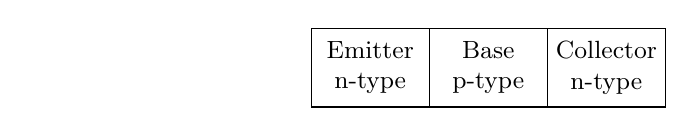
\begin{tikzpicture}
            \draw
                (0,0)
                    rectangle ++(1.5,1.0)
                        node[pos=0.5, align=center, font={\small}]{Emitter \\ n-type}
                    rectangle ++(1.5,-1.0)
                        node[pos=0.5, align=center, font={\small}]{Base \\ p-type}
                    rectangle ++(1.5,1.0)
                        node[pos=0.5, align=center, font={\small}]{Collector \\ n-type}
            ;
            \path
                (0,0) -- (-3.6,0)
            ;
        \end{tikzpicture}
        \end{center}

        \begin{minipage}[c]{0.76\columnwidth}
            \MinipageInheritDocumentFormatting
            \emph{Forward active} DC characteristics:
            \begin{gather*}
                \begin{gathered}
                    I_C = \beta I_B
                    \\
                    I_E = \parens{\beta + 1} I_B
                \end{gathered}
                \qquad\quad
                \begin{gathered}
                    \beta = \frac{\alpha}{1 - \alpha}
                    \\
                    I_C = \alpha I_E
                \end{gathered}
            \end{gather*}

            Large signal \emph{base-width modulation}:
            \vspace*{-2mm}
            \begin{gather*}
                I_C
                = I_S e^{\brackets*{V_{BE} \mathbin{/} V_T}}
                \parens*{1 + \frac{V_{CE}}{V_A}}
            \end{gather*}
        \end{minipage}%
        \begin{minipage}[c]{0.24\columnwidth}
            \MinipageInheritDocumentFormatting
            \begin{circuitikz}
                \draw
                    (0,0)
                        node[npn, anchor=center](Q1){}
                    (Q1.B)
                        -- ++(-0.2,0)
                            node[currarrow, label=above:$I_B$]{}
                        -- ++(-0.4,0)
                            node[ocirc, label=left:B]{}
                    (Q1.E)
                        -- ++(0,-0.2)
                            node[currarrow, label=left:$I_E$, rotate=-90]{}
                        -- ++(0,-0.6)
                            node[ocirc, label=below:E]{}
                    (Q1.C)
                        -- ++(0,0.2)
                            node[currarrow, label=left:$I_C$, rotate=-90]{}
                        -- ++(0,0.6)
                            node[ocirc, label=above:C]{}
                ;
            \end{circuitikz}
        \end{minipage}
        \smallskip

        {\footnotesize\myul{\textbf{Hybrid-$\pi$ Small Signal Model}}}
        \begin{center}
        \begin{circuitikz}
            \draw
                (0,0)
                        node[ocirc, label=left:B]{}
                    -- ++(1,0)
                        coordinate(B1)
                    to[C, l_=$C_\pi$] ++(0,-2)
                    -- ++(3.2,0)
                        coordinate(E)
                    -- ++(2.2,0)
                    to[R, l_=$r_o$] ++(0,2)
                        coordinate(C)
                    -- ++(1,0)
                        node[ocirc, label=right:C]{}
                (B1)
                    -- ++(1.2,0)
                        coordinate(B2)
                    to[R, l_=$r_\pi$, v^>=$v_{BE}$] ++(0,-2)
                (B2)
                    to[C, l=$C_\mu$] (E |- C)
                    %to[american controlled current source, l=$g_m v_{BE}$] (E)
                    to[american controlled current source, l=$
                            \begin{gathered}
                                g_m v_{BE} \\
                                \textbf{\small (or)} \\
                                \beta i_B
                            \end{gathered}
                        $] (E)
                (E |- C)
                    -- (C)
                (E)
                    -- ++(0,-1)
                        node[ocirc, label=right:E]{}

                (B1)
                    ++(-0.5,0)
                        node[currarrow, label=above:$i_B$]{}
                (C)
                    ++(0.5,0)
                        node[currarrow, label=above:$i_C$, rotate=180]{}
                (E)
                    ++(0,-0.5)
                        node[currarrow, label=left:$i_E$, rotate=-90]{}
            ;
        \end{circuitikz}
        \end{center}
        \begin{gather*}
            g_m = \frac{\abs*{I_C}}{V_T}
            \qquad\quad
            r_\pi = \frac{\beta}{g_m}
            \qquad\quad
            r_o = \frac{V_{CE} + V_A}{I_C}
        \end{gather*}

        Transition frequency:
        \begin{gather*}
            f_T = \frac{g_m}{2 \pi \parens{C_\pi + C_\mu}}
        \end{gather*}

        \MulticolsBreak

        \myul{PNP Type}

        \begin{center}
        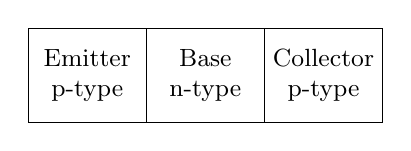
\begin{tikzpicture}
            \draw
                (0,0)
                    rectangle ++(1.5,1.2)
                        node[pos=0.5, align=center, font={\small}]{Emitter \\ p-type}
                    rectangle ++(1.5,-1.2)
                        node[pos=0.5, align=center, font={\small}]{Base \\ n-type}
                    rectangle ++(1.5,1.2)
                        node[pos=0.5, align=center, font={\small}]{Collector \\ p-type}
            ;
        \end{tikzpicture}

        \begin{circuitikz}
            \draw
                (0,0)
                    node[pnp, anchor=center, yscale=-1](Q2){}
                (Q2.B)
                    node[ocirc, label=left:B]{}
                (Q2.E)
                    node[ocirc, label=below:E]{}
                (Q2.C)
                    node[ocirc, label=above:C]{}
            ;
        \end{circuitikz}
        \end{center}

        \Todo{Write up on this soon!}

        \Todo{Also, we should maybe derive the hybrid-$\pi$ model and show the unsimplified version in the extras section?}

        \MulticolsCleanEnd
    \end{MulticolsSoftSepRule}
    \MulticolsReduceVspaceAfter

    Basic modes:
    \begin{itemize}
        \item \emph{Forward Active} (BE forward-biased, BC reverse-biased)
        \item \emph{Reverse Active} (BE reverse-biased, BC forward-biased)
        \item \emph{Saturation} (both junctions forward-biased)
        \item \emph{Cut-off} (both junctions reverse-biased)
    \end{itemize}

\end{CheatsheetEntryFrame}

\newpage

\begin{CheatsheetEntryFrame}

    \CheatsheetEntryTitle{MOSFET}

    \begin{MulticolsSoftSepRule}{2}
        \myul{N-Channel Type (NMOS)}

        \begin{minipage}[c]{0.76\columnwidth}
            \MinipageInheritDocumentFormatting
            Device parameters:
            \begin{gather*}
                k_n = \mu_n C_{ox}
                \qquad
                \lambda = \frac{1}{V_A + V_{DS}}
            \end{gather*}

            \emph{Saturation region} DC characteristics:
            \begin{gather*}
                I_G = 0
                \\
                \begin{aligned}
                    I_{DS}
                        &= \frac{1}{2} k_n \frac{W}{L}
                        \parens{V_{GS} - V_t}^2
                        \parens{1 + \lambda V_{DS}}
                        \\
                    &\approx \frac{1}{2} k_n \frac{W}{L}
                        \parens{V_{GS} - V_t}^2
                        \qquad \text{\footnotesize{}(if $\lambda \to 0$)}
                \end{aligned}
            \end{gather*}
        \end{minipage}%
        \begin{minipage}[c]{0.24\columnwidth}
            \MinipageInheritDocumentFormatting
            \begin{circuitikz}
                \draw
                    (0,0)
                        node[nmos, anchor=center](Q1){}
                    (Q1.G)
                        node[ocirc, label=left:G]{}
                    (Q1.S)
                        node[ocirc, label=below:S]{}
                    (Q1.D)
                        node[ocirc, label=above:D]{}
                ;
            \end{circuitikz}
        \end{minipage}
        \smallskip

        \emph{Overdrive voltage}: $V_{OV} = V_{GS} - V_t$
        \smallskip

        {\footnotesize\myul{\textbf{Small Signal Model}}}
        \begin{center}
        \begin{circuitikz}
            %\tikzset{/tikz/circuitikz/bipoles/length=1.2cm}
            \draw
                (0,0)
                        node[ocirc, label=above:G]{}
                    -- ++(1,0)
                        coordinate(G)
                    to[C, l_=$C_{GS}$, v^>=$V_{GS}$] ++(0,-2)
                    -- ++(2.2,0)
                        coordinate(S)
                    -- ++(2.2,0)
                    to[R, l_=$r_o$] ++(0,2)
                        coordinate(D)
                    -- ++(1,0)
                        node[ocirc, label=above:D]{}
                (G)
                    to[C, l=$C_{GD}$] (S |- D)
                    to[american controlled current source, l=$g_m V_{GS}$] (S)
                (S |- D)
                    -- (D)
                (S)
                    -- ++(0,-1)
                        node[ocirc, label=right:S]{}
            ;
        \end{circuitikz}
        \end{center}
        \begin{gather*}
            g_m
            = k_n \frac{W}{L} \parens{V_{GS} - V_t}
            = \sqrt{2 k_n \frac{W}{L} I_{DS}}
            \\
            r_o
            = \frac{1}{\lambda I_{DS}}
            = \frac{V_A + V_{DS}}{I_{DS}}
        \end{gather*}

        \MulticolsBreak

        \myul{P-Channel Type (PMOS)}

        \begin{center}
        \begin{circuitikz}
            \draw
                (0,0)
                    node[pmos, anchor=center](Q2){}
                (Q2.G)
                    node[ocirc, label=left:G]{}
                (Q2.S)
                    node[ocirc, label=above:S]{}
                (Q2.D)
                    node[ocirc, label=below:D]{}
            ;
        \end{circuitikz}
        \end{center}

        \Todo{Write up on this soon!}

        \Todo{Also add discussion on enhancement/depletion-type MOSFETs?}

        \MulticolsCleanEnd
    \end{MulticolsSoftSepRule}
    \MulticolsReduceVspaceAfter

\end{CheatsheetEntryFrame}

\begin{CheatsheetEntryFrame}

    \CheatsheetEntryTitle{Miller Theorem}

    \Todo{This?}

\end{CheatsheetEntryFrame}

\Todo{(for the next page) Write something better than ``external capacitors" and ``intrinsic capacitors"? E.g. for mid-band analysis, do we just short $\si{\micro\farad}$ capacitors?}

\newpage

\begin{CheatsheetEntryFrame}

    \CheatsheetEntryTitle{Transistor Amplifier General Analysis Method} \CheatsheetEntrySubtitle{(for linear operation)}
    \bigskip

    \begin{center}
    \begin{tikzpicture}[node distance=2cm]
        \node (step1) [MyFlowchartProcess, align=center]
            {DC Analysis \\ \footnotesize (Finding Q-point values)} (step1);
        \node (step2) [MyFlowchartProcess, below of=step1, align=center]
            {Calculate Small Signal Parameters};
        \node (step3b) [MyFlowchartProcess, below of=step2, align=center]
            {Mid-Frequency \\ Analysis};
        \node (step3a) [MyFlowchartProcess, left of=step3b, align=center, xshift=-2cm]
            {Low-Frequency \\ Analysis};
        \node (step3c) [MyFlowchartProcess, right of=step3b, align=center, xshift=2cm]
            {High-Frequency \\ Analysis};

        \draw[MyFlowchartArrow] (step1) -- (step2);
        \draw[MyFlowchartArrow] (step2) -- (step3a);
        \draw[MyFlowchartArrow] (step2) -- (step3b);
        \draw[MyFlowchartArrow] (step2) -- (step3c);

        %% TODO: Make this work? The problem is, I need to make line breaks.
        %\node (tab) [align=center, right of=step2, xshift=4cm, yshift=1cm] {\scalebox{0.8}{%
        %    \begin{tabular}{|c|c|c|c|}
        %        \hline
        %        & DC Sources & AC Sources & Transistors \\\hline 
        %        DC Analysis & enable  & disable & unchanged \\\hline 
        %        Low-Freq    & disable & enable  & small signal model \\\hline
        %        Mid-Freq    & disable & enable  & small signal model \\\hline
        %        High-Freq   & disable & enable  & small signal model \\\hline
        %    \end{tabular}%
        %}};
    \end{tikzpicture}
    \end{center}

    \bigskip

    \newcommand{\TmpFormatYes}[1]{\textbf{\color{mygreen}#1}}
    \newcommand{\TmpFormatNo}[1]{\textbf{\color{myred}#1}}
    \newcommand{\TmpFormatAltA}[1]{\textbf{\color{myblue}#1}}
    \newcommand{\TmpFormatAltB}[1]{\textbf{\color{mypurple}#1}}
    \newcommand{\TmpFormatAltC}[1]{\textbf{\color{myorange}#1}}

    For each type of analysis, \myul{first reinterpret/redraw the circuit as follows}:
    \begin{center}
    \begin{tabular}{|c|c|c|c|c|c|}
        \cline{2-6}
        \multicolumn{1}{c|}{}
            & \thead{DC \\ Sources}
            & \thead{AC \\ Sources}
            & \thead{Transistors}
            & \thead{External/$\si{\micro\farad}$ \\ Capacitors}
            & \thead{Intrinsic \\ Capacitors} \\\hline 
        \thead{DC Analysis}
            & \TmpFormatYes{enable}
            & \TmpFormatNo{disable}
            & \TmpFormatYes{unchanged}
            & \TmpFormatAltC{open}
            & \TmpFormatAltC{open} \\\hline 
        \thead{Low-Freq}
            & \TmpFormatNo{disable}
            & \TmpFormatYes{enable}
            & \TmpFormatAltA{small signal model} %\makecell{small signal \\ model}
            & \TmpFormatYes{keep}
            & \TmpFormatAltC{open} \\\hline
        \thead{Mid-Freq}
            & \TmpFormatNo{disable}
            & \TmpFormatYes{enable}
            & \TmpFormatAltA{small signal model}
            & \TmpFormatAltB{short}
            & \TmpFormatAltC{open} \\\hline
        \thead{High-Freq}
            & \TmpFormatNo{disable}
            & \TmpFormatYes{enable}
            & \TmpFormatAltA{small signal model}
            & \TmpFormatAltB{short}
            & \TmpFormatYes{keep} \\\hline
    \end{tabular}
    \end{center}

    %{\footnotesize External capacitors are $\si{\micro\farad}$ capacitors outside of the transistors. Intrinsic capacitors are capacitances found in the transistor small signal model.}
    
    \bigskip
    \SoftHLine
    %\bigskip

    \begin{MulticolsSoftSepRule}{2}

        \myul{DC Analysis}
        \begin{enumerate}
            \item Assume linear operation:
            \begin{itemize}
                \item BJTs are \emph{forward active}.
                \item MOSFETs are in \emph{saturation}.
            \end{itemize}
            \item Apply circuit analysis to find:
            \begin{itemize}
                \item $I_C$ and $V_{CE}$ {\footnotesize {}[for NPN BJTs]}
                \item $I_D$ and $V_{DS}$ {\footnotesize {}[for N-Channel MOSFETs]}
            \end{itemize}
            \item Check that the linear operation assumptions are met.
        \end{enumerate}

        \bigskip
        \SoftHLine
        \bigskip

        \myul{Mid-Frequency Analysis}

        Analyze the circuit to find:
        \begin{itemize}
            \item gain
            \item input/output resistance
        \end{itemize}

        %\bigskip
        %\SoftHLine
        %\bigskip
        \MulticolsBreak

        \myul{Low-Frequency Analysis}

        \emph{Short circuit time constant method} to find the \linebreak lower cut-off frequency $f_L$:
        \begin{gather*}
            f_L
            = \frac{1}{2 \pi}
            \sum_{i=1}^n \frac{1}{\tau_i}
            \qquad
            \tau_i = C_i R_{sci}
        \end{gather*}
        Calculate a $\tau_i$ for every capacitor $C_i$.

        $R_{sci}$ is the Th\'evenin resistance seen by $C_i$ \linebreak with all other capacitors \textbf{\myul{shorted}}.

        \bigskip
        \SoftHLine
        \bigskip

        \myul{High-Frequency Analysis}

        \emph{Open circuit time constant method} to find the \linebreak upper cut-off frequency $f_H$:
        \begin{gather*}
            f_H
            = \frac{1}{
                \displaystyle
                \brackets*{
                    2 \pi \sum_{i=1}^n \tau_i
                }
            }
            \qquad
            \tau_i = C_i R_{oci}
        \end{gather*}
        Calculate a $\tau_i$ for every capacitor $C_i$.

        $R_{oci}$ is the Th\'evenin resistance seen by $C_i$ \linebreak with all other capacitors \textbf{\myul{opened}}.
        
        %\MulticolsCleanEnd % TODO: Why is this not needed?
    \end{MulticolsSoftSepRule}
\end{CheatsheetEntryFrame}

 }

\newpage
\section{Electrical Engineering: Digital Systems}
\label{sec:ee-digital}

    { \subsection{Digital Circuits and Logic}%
\label{sub:digital-circuits-and-logic}

\begin{multicols}{2}

    \CheatsheetEntryFrame{

        \renewcommand{\MyReusableFormatting}[5]{ % This will be used for content
            %\vspace*{1ex}
            \begin{minipage}[c]{0.20\columnwidth}
                \centering
                #1
            \end{minipage}%
            \begin{minipage}[c]{0.18\columnwidth}
                \centering
                #2
            \end{minipage}%
            %\hspace{0.04\columnwidth}%
            \begin{minipage}[c]{0.32\columnwidth}
                \centering
                \scalebox{0.8}{%
                \begin{tabular}{#3}
                    \HLineA
                    #4
                    \HLineA
                \end{tabular}
                }%
            \end{minipage}%
            \begin{minipage}[c]{0.30\columnwidth}
            \begin{center}
                \begin{circuitikz}
                    \draw
                        #5
                    ;
                \end{circuitikz}
            \end{center}
            \end{minipage}%
            \vspace*{1ex}
        }
        \renewcommand{\MyReusableFormattingB}{ % This will be used for separators
            {\color{lightgray} \hrule{}}
        }
        \renewcommand{\MyReusableFormattingC}{ % This will be used for special separators
            \MyReusableFormattingB%
            \vspace*{2.5pt}%
            \MyReusableFormattingB
        }

        \renewcommand{\X}{{\cellcolor{myred}\color{white}$\bm{0}$}} % Used for logical low
        \renewcommand{\Y}{{\cellcolor{mygreen}\color{white}$\bm{1}$}} % Used for logical high

        \renewcommand{\W}[1]{{\cellcolor{black}\color{white}$\bm{#1}$}} % Used for headings

        \renewcommand{\VRuleA}{\vrule width 3pt}
        \renewcommand{\HLineA}{\noalign{\hrule height 3pt}}

        \CheatsheetEntryTitle{Logic Gates}

        \MyReusableFormatting{NOT {\footnotesize(Inverter)}}{$\overline{A}$}{!{\VRuleA}c!{\VRuleA}c!{\VRuleA}}{
            \W{A} & \W{O} \\ \HLineA
            \X & \Y \\
            \Y & \X \\
        }{
            (0,0) node[american not port, name=G, /tikz/circuitikz/bipoles/length=1.0cm, /tikz/circuitikz/bipoles/not port/circle width=0.35] {}
            (G.in)  -- ++(-0.4,0)
            (G.out) -- ++( 0.4,0)
        }
        \MyReusableFormattingC

        \MyReusableFormatting{AND}{$A \cdot B$}{!{\VRuleA}cc!{\VRuleA}c!{\VRuleA}}{
            \W{A} & \W{B} & \W{O} \\ \HLineA
            \X & \X & \X \\
            \X & \Y & \X \\
            \Y & \X & \X \\
            \Y & \Y & \Y \\
        }{
            (0,0) node[american and port, name=G] {}
            (G.in 1) -- ++(-0.4,0)
            (G.in 2) -- ++(-0.4,0)
            (G.out)  -- ++( 0.4,0)
        }
        \MyReusableFormattingB

        \MyReusableFormatting{OR}{$A + B$}{!{\VRuleA}cc!{\VRuleA}c!{\VRuleA}}{
            \W{A} & \W{B} & \W{O} \\ \HLineA
            \X & \X & \X \\
            \X & \Y & \Y \\
            \Y & \X & \Y \\
            \Y & \Y & \Y \\
        }{
            (0,0) node[american or port, name=G] {}
            (G.in 1) -- ++(-0.4,0)
            (G.in 2) -- ++(-0.4,0)
            (G.out)  -- ++( 0.4,0)
        }
        \MyReusableFormattingB

        \MyReusableFormatting{XOR}{$A \oplus B$}{!{\VRuleA}cc!{\VRuleA}c!{\VRuleA}}{
            \W{A} & \W{B} & \W{O} \\ \HLineA
            \X & \X & \X \\
            \X & \Y & \Y \\
            \Y & \X & \Y \\
            \Y & \Y & \X \\
        }{
                (0,0) node[american xor port, name=G] {}
                (G.in 1) -- ++(-0.4,0)
                (G.in 2) -- ++(-0.4,0)
                (G.out)  -- ++( 0.4,0)
        }

        \MyReusableFormattingC

        \MyReusableFormatting{NAND}{$\overline{A \cdot B}$}{!{\VRuleA}cc!{\VRuleA}c!{\VRuleA}}{
            \W{A} & \W{B} & \W{O} \\ \HLineA
            \X & \X & \Y \\
            \X & \Y & \Y \\
            \Y & \X & \Y \\
            \Y & \Y & \X \\
        }{
            (0,0) node[american nand port, name=G] {}
            (G.in 1) -- ++(-0.4,0)
            (G.in 2) -- ++(-0.4,0)
            (G.out)  -- ++( 0.4,0)
        }
        \MyReusableFormattingB

        \MyReusableFormatting{NOR}{$\overline{A + B}$}{!{\VRuleA}cc!{\VRuleA}c!{\VRuleA}}{
            \W{A} & \W{B} & \W{O} \\ \HLineA
            \X & \X & \Y \\
            \X & \Y & \X \\
            \Y & \X & \X \\
            \Y & \Y & \X \\
        }{
            (0,0) node[american nor port, name=G] {}
            (G.in 1) -- ++(-0.4,0)
            (G.in 2) -- ++(-0.4,0)
            (G.out)  -- ++( 0.4,0)
        }
        \MyReusableFormattingB

        \MyReusableFormatting{XNOR}{$\overline{A \oplus B}$}{!{\VRuleA}cc!{\VRuleA}c!{\VRuleA}}{
            \W{A} & \W{B} & \W{O} \\ \HLineA
            \X & \X & \Y \\
            \X & \Y & \X \\
            \Y & \X & \X \\
            \Y & \Y & \Y \\
        }{
            (0,0) node[american xnor port, name=G] {}
            (G.in 1) -- ++(-0.4,0)
            (G.in 2) -- ++(-0.4,0)
            (G.out)  -- ++( 0.4,0)
        }

    }

    \MulticolsBreak

    \CheatsheetEntryFrame{

        \CheatsheetEntryTitle{Binary Numbers}

        \Todo{This!}

        \CheatsheetEntryExtraSeparation

        \CheatsheetEntryTitle{Hexadecimal and Octal Numbers}

        \Todo{This!}

    }

    \CheatsheetEntryFrame{

        %\CheatsheetEntryTitle{Commutative Laws}
        %\begin{gather*}
        %    A \cdot B = B \cdot A \\
        %    A + B = B + A
        %\end{gather*}

        %\CheatsheetEntryTitle{Associative Laws}
        %\begin{gather*}
        %    (A \cdot B) \cdot C = A \cdot (B \cdot C) = A \cdot B \cdot C \\
        %    (A + B) + C = A + (B + C) = A + B + C
        %\end{gather*}

        \CheatsheetEntryTitle{Distributive Laws}
        \begin{gather*}
            A \cdot (B + C) = (A \cdot B) + (A \cdot C) \\
            A + (B \cdot C) = (A + B) \cdot (A + C)
        \end{gather*}

        \CheatsheetEntryTitle{Absorption Laws}
        \begin{gather*}
            A + (A \cdot B) = A \\
            A \cdot (A + B) = A \\
            (A \cdot B) + (A \cdot \overline{B}) = A \\
            (A + B) \cdot (A + \overline{B}) = A
        \end{gather*}

        \CheatsheetEntryTitle{De Morgan's Theorem}
        \begin{gather*}
            \overline{A + B} = \overline{A} \cdot \overline{B} \\
            \overline{A \cdot B} = \overline{A} + \overline{B}
        \end{gather*}

    }

\end{multicols}

 }

\newpage
\section{Computer Science}
\label{sec:compsci}

    { \subsection{Databases: The Relational Model, Relational Algebra, and some SQL}%
\label{sub:relational-algebra}

\begin{multicols}{2}

    % TODO: Find a way to work this into this cheatsheet.
    %\begin{CheatsheetEntryFrameNew}

    %    \CheatsheetEntryTitle{Relations}

    %    The term \textit{relation} can refer to either:
    %    \begin{itemize}
    %        \item a \textit{relation schema}, or
    %        \item a \textit{relation instance}.
    %    \end{itemize}

    %    Intended usage should be clear from context.

    %\end{CheatsheetEntryFrameNew}

    \begin{CheatsheetEntryFrame}

        \CheatsheetEntryTitle{Relation Schemas}

        Relation schemas are \ul{unordered sets} of \textit{attributes}.

        Notation for relation $R$ and attributes $A, B, C, \dots$:
        \begin{equation*}
            R(A, B, C, \dots)
        \end{equation*}
        %% I want a visually annotated version like this below.
        %% Problem is that the relation name annotation looks really awkward.
        %\newcommand{\X}{\rule{0mm}{1.1em}}
        %\begin{equation*}
        %    {
        %        \color{mycontrastred}
        %        \overbrace{\color{black} \X \hspace{1em} R}^{\mathclap{\substack{\textbf{\textit{relation}}\\\textbf{\textit{name}}}}}
        %    }
        %    ({
        %        \color {mycontrastpurple}
        %        \overbrace{\color{black} \X A, B, C, \dots}^{\textbf{\textit{attributes}}}
        %    })
        %\end{equation*}

        %% TODO: Somehow work something like this in?
        %Practical example:
        %\begin{center}
        %    \ttd{Accounts(branch, accountno, balance)}
        %    %% The original visually annotated version.
        %    %% No longer used since it's already described elsewhere.

        %    %\newcommand{\X}{\rule{0mm}{1.1em}}

        %    %$\color{mycontrastred} \overbrace{\color{black} \X \texttt{Accounts}}^{\substack{\textbf{\textit{relation}}\\\textbf{\textit{name}}}}$\texttt{(}$\color {mycontrastpurple} \overbrace{\color{black} \X \texttt{branch, accountno, balance}}^{\textbf{\textit{attributes}}}$\texttt{)}
        %\end{center}

        \SubsectionFrameAddSeparation
        \begin{SqlSubsection}{SQL Create Relation (Examples)}
            \begin{CheatsheetSubsectionLst}
                CREATE TABLE Accounts (
                    branch      VARCHAR(20),
                    accountno   CHAR(7)       PRIMARY KEY,
                    balance     NUMERIC       NOT NULL,

                    CONSTRAINT accountnoformat CHECK(
                        accountno ~ '[A-Z]-[0-9]{5}'
                    )
                );
            \end{CheatsheetSubsectionLst}

            \medskip
            {\footnotesize Note: The \texttt{\textasciitilde} regex operator is specific to \textit{PostgreSQL}.}
            %% Would be nice if an explanation of syntax could be worked in...
            %\medskip
            %Syntax:
            %\begin{CheatsheetSubsectionLst}
            %    CREATE TABLE <tablename> (
            %        <attribute> <data type> <constraints>,
            %        <attribute> <data type> <constraints>,
            %        <...>
            %        <table-level constraint>,
            %        <table-level constraint>,
            %        <...>
            %    );
            %\end{CheatsheetSubsectionLst}
        \end{SqlSubsection}
        \SubsectionFrameReduceSkip
        \begin{SqlSubsection}{SQL Remove Relation (Example)}%
            \begin{CheatsheetSubsectionLst}
                DROP TABLE Accounts;
            \end{CheatsheetSubsectionLst}
        \end{SqlSubsection}

    \end{CheatsheetEntryFrame}

    \begin{CheatsheetEntryFrame}

        \CheatsheetEntryTitle{Attributes}

        Attributes are labels for parts of a schema.

        The \textit{domain} of an attribute is the set of values that can be associated with the attribute.

        For attribute $A$, this is denoted:
        \begin{equation*}
            \dom{(A)}
        \end{equation*}

        \SubsectionFrameReduceSkip
        \begin{SqlSubsection}{Some Common SQL Data Types and Constraints}
            \newcommand{\SqlOptionalPart}[1]{{\color{SqlSubsectionTextColorGrayed}(p,s)}}
            \texttt{INTEGER, SMALLINT, BIGINT, NUMERIC\SqlOptionalPart{(p,s)},}\\[0mm]
            \texttt{REAL, DOUBLE PRECISION, FLOAT\SqlOptionalPart{(p)},}\\[0mm]
            \texttt{CHAR(n), VARCHAR(n), CLOB,}\\[0mm]
            \texttt{BOOLEAN, BINARY(n), VARBINARY(n), BLOB,}\\[0mm]
            \texttt{DATE, TIME, TIMESTAMP, INTERVAL.}
        \end{SqlSubsection}
        %% Would be nice to add something like this, but I can't really fit it in while also having it be sufficiently useful.
        %\SubsectionFrameReduceSkip
        %\begin{SqlSubsection}{Some Common SQL Constraints}
        %    \SubsectionFrameTableRemoveSpace
        %    \begin{tabularx}{\textwidth}{X|X}
        %        Column Constraint & Table Constraint \\ \hline
        %        \texttt{NOT NULL} & \texttt{NOT NULL (col)} \\
        %        \texttt{PRIMARY KEY} & \texttt{PRIMARY KEY (col)} \\
        %        \texttt{UNIQUE} & \texttt{UNIQUE (col, ...)} \\
        %        \texttt{REFERENCES rel(col)} & \texttt{FOREIGN KEY (col) REFERENCES rel(col)}
        %    \end{tabularx}
        %    \SubsectionFrameTableRemoveSpace
        %\end{SqlSubsection}

    \end{CheatsheetEntryFrame}

    %\Todo{Discuss the domain of the whole schema?}

    \MulticolsBreak

    \begin{CheatsheetEntryFrame}

        \CheatsheetEntryTitle{Relation Instances}

        Relation instances are \ul{unordered sets} of \textit{tuples}.

        To show that $r$ is an instance of relation $R$, we write:
        \begin{equation*}
            r(R)
        \end{equation*}

        %Tuples are mappings from schema $R$ to domain $\dom{(R)}$.

        \SubsectionFrameRemoveSeparation
        \begin{SqlAltSubsection}{Example Database}
        \begin{center}
            \newcommand{\Y}{0.44}
            \newcommand{\Yhalf}{0.22}
            \newcommand{\MyTableCell}[3]{%
                (R#1 -| C#2) node[right, align=left, font=\footnotesize] {\vphantom{$M_I^{I^x}$}\texttt{#3}}%
            }
            \begin{tikzpicture}[scale=1, transform shape]
                \path
                    (0,0)      coordinate (LeftEdge)
                    ++(0.08,0) coordinate (C1)
                    ++(1.98,0) coordinate (C2)
                    ++(1.50,0) coordinate (C3)
                    ++(2.10,0) coordinate (RightEdge)
                    ++(0.20,0) coordinate (RightOS1)
                    ++(0.50,0) coordinate (RightOS2)
                ;
                \begin{scope}[shift={(0,0)}]
                    \path
                        (0,0)         coordinate (Top)
                        ++(0,-\Yhalf) coordinate (RA)
                        ++(0,-\Yhalf) coordinate (Bottom)

                        (Top)
                        ++(0, 0.040) % Slight extra offset
                        ++(0, \Yhalf) coordinate (RT) % Title row

                        (Top)
                        ++(0,-0.1) coordinate (TopOS1)

                        (Top)
                        ++(0,1.2) coordinate (TopOS2)
                        ++(0,0.5) coordinate (TopOS3)
                    ;
                    \draw
                        (Top -| LeftEdge) rectangle (RightEdge |- Bottom)
                    ;
                    \draw
                        \MyTableCell{T}{1}{\textbf{Customers}}

                        \MyTableCell{A}{1}{customerid}
                        \MyTableCell{A}{2}{name}
                        \MyTableCell{A}{3}{address}
                    ;
                \end{scope}
                \begin{scope}[shift={(0,-0.52)}]
                    \path
                        (0,0)         coordinate (Top)
                        ++(0,-\Yhalf) coordinate (R1)
                        ++(0,-\Y)     coordinate (R2)
                        ++(0,-\Y)     coordinate (R3) coordinate (HorizontalMid)
                        ++(0,-\Y)     coordinate (R4)
                        ++(0,-\Y)     coordinate (R5)
                        ++(0,-\Yhalf) coordinate (Bottom)
                    ;
                    \draw
                        (Top -| LeftEdge) rectangle (RightEdge |- Bottom)
                    ;
                    \draw
                        \MyTableCell{1}{1}{1774504}
                        \MyTableCell{1}{2}{Amy}
                        \MyTableCell{1}{3}{Surry Hills}

                        \MyTableCell{2}{1}{4389167}
                        \MyTableCell{2}{2}{Chris}
                        \MyTableCell{2}{3}{Richmond}

                        \MyTableCell{3}{1}{4622780}
                        \MyTableCell{3}{2}{Josh}
                        \MyTableCell{3}{3}{North Ryde}
                        
                        \MyTableCell{4}{1}{5691729}
                        \MyTableCell{4}{2}{Sam}
                        \MyTableCell{4}{3}{Kensington}

                        \MyTableCell{5}{1}{9527291}
                        \MyTableCell{5}{2}{Vanessa}
                        \MyTableCell{5}{3}{Richmond}
                    ;

                    \draw[mycontrastblue]
                        (HorizontalMid -| RightOS2)
                        ++(0.10,0) coordinate (RowArrowConvg)
                        ++(0.05,0) node[right, align=left, font=\small] {
                            \textbf{\textit{tuples,}} \\
                            \textbf{\textit{rows,}} \\
                            \textbf{\textit{records}}
                        }
                    ;
                    \draw[-stealth, cap=round, line width=2.0pt, mycontrastblue] (R1 -| RightOS2) -- (R1 -| RightOS1);
                    \draw[-stealth, cap=round, line width=2.0pt, mycontrastblue] (R2 -| RightOS2) -- (R2 -| RightOS1);
                    \draw[-stealth, cap=round, line width=2.0pt, mycontrastblue] (R3 -| RightOS2) -- (R3 -| RightOS1);
                    \draw[-stealth, cap=round, line width=2.0pt, mycontrastblue] (R4 -| RightOS2) -- (R4 -| RightOS1);
                    \draw[-stealth, cap=round, line width=2.0pt, mycontrastblue] (R5 -| RightOS2) -- (R5 -| RightOS1);
                    \draw[          cap=round, line width=2.0pt, mycontrastblue] (R1 -| RightOS2) -- (R5 -| RightOS2);
                    %\draw[         cap=round, line width=2.0pt, mycontrastblue] (RowArrowConvg) -- (RowArrowConvg -| RightOS2);

                    \draw[mycontrastpurple]
                        (TopOS2 -| C3)
                        ++(1.8, 0) coordinate (ColArrowConvgRef)
                        ++(0.05, 0) node[right, align=left, font=\small] {
                            \textbf{\textit{attributes,}} \\
                            \textbf{\textit{columns,}} \\
                            \textbf{\textit{fields}}
                        }
                    ;
                    \path
                        (RA -| C1) ++(1.75, 0.30) coordinate (ColArrowEnd1)
                        (RA -| C2) ++(0.85, 0.30) coordinate (ColArrowEnd2)
                        (RA -| C3) ++(0.80, 0.30) coordinate (ColArrowEnd3)
                        (ColArrowConvgRef) ++(0, -0.1) coordinate (ColArrowConvg)
                    ;
                    \draw[-stealth, cap=round, line width=2.0pt, mycontrastpurple] (ColArrowConvg) -- (ColArrowEnd1);
                    \draw[-stealth, cap=round, line width=2.0pt, mycontrastpurple] (ColArrowConvg) -- (ColArrowEnd2);
                    \draw[-stealth, cap=round, line width=2.0pt, mycontrastpurple] (ColArrowConvg) -- (ColArrowEnd3);

                    \draw[mycontrastred]
                        (TopOS3 -| C2)
                        ++(0.30, 0) coordinate (RelArrowConvgRef)
                        ++(0.05, 0) node[right, align=left, font=\small] {
                            \textbf{\textit{relation,}} \\
                            \textbf{\textit{table}}
                        }
                    ;
                    \path
                        (RT -| C1) ++(1.00, 0.25) coordinate (RelArrowEnd)
                        (RelArrowConvgRef) ++(0, -0.3) coordinate (RelArrowConvg)
                    ;
                    \draw[-stealth, cap=round, line width=2.0pt, mycontrastred] (RelArrowConvg) -- (RelArrowEnd);

                    % An attempt was made to make smooth lines...
                    %\draw[-stealth, cap=round, line width=1.5pt]
                    %    plot [smooth] coordinates { (RowArrowConvg) (R1 -| RightOS2) (R1 -| RightOS1) };
                    %\draw[-stealth, cap=round, line width=1.5pt]
                    %    plot [smooth] coordinates { (RowArrowConvg) (R2 -| RightOS2) (R2 -| RightOS1) };
                    %\draw[-stealth, cap=round, line width=1.5pt]
                    %    plot [smooth] coordinates { (RowArrowConvg) (R3 -| RightOS2) (R3 -| RightOS1) };
                    %\draw[-stealth, cap=round, line width=1.5pt]
                    %    plot [smooth] coordinates { (RowArrowConvg) (R4 -| RightOS2) (R4 -| RightOS1) };
                    %\draw[-stealth, cap=round, line width=1.5pt]
                    %    plot [smooth] coordinates { (RowArrowConvg) (R5 -| RightOS2) (R5 -| RightOS1) };
                \end{scope}
            \end{tikzpicture}

            \medskip

            {\footnotesize%
            \begin{tabular}{|llr|}
                \multicolumn{3}{l}{\ttd{Accounts}}
                    \\ \hline
                \multicolumn{1}{|l}{\ttd{branch}}
                    & \multicolumn{1}{l}{\ttd{accountno}}
                    & \multicolumn{1}{l|}{\ttd{balance}}
                    \\ \hline\hline
                \ttd{Richmond}
                    & \ttd{A-02772}
                    & \ttd{20.87}
                    \\
                \ttd{Macquarie} % The actual suburb is called Macquarie Park, but I want a smaller table.
                    & \ttd{J-31553}
                    & \ttd{60899.58}
                    \\
                \ttd{Richmond}
                    & \ttd{W-40018}
                    & \ttd{84731.08}
                    \\
                \ttd{Haymarket}
                    & \ttd{A-74884}
                    & \ttd{483.94}
                    \\
                \ttd{Haymarket}
                    & \ttd{P-85953}
                    & \ttd{7294.62}
                    \\ \hline
            \end{tabular}%

            \medskip
            %\hspace{2.0ex} % TODO: Prefer to instead make these two tables side-by-side if possible.

            \begin{tabular}{|ll|}
                \multicolumn{2}{l}{\ttd{HeldBy}}
                    \\ \hline
                \multicolumn{1}{|l}{\ttd{accountno}}
                    & \multicolumn{1}{l|}{\ttd{owner}}
                    \\ \hline\hline
                \ttd{A-02772}
                    & \ttd{4389167}
                    \\
                \ttd{A-02772}
                    & \ttd{9527291}
                    \\
                \ttd{J-31553}
                    & \ttd{4622780}
                    \\
                \ttd{W-40018}
                    & \ttd{4389167}
                    \\
                \ttd{W-40018}
                    & \ttd{9527291}
                    \\
                \ttd{A-74884}
                    & \ttd{1774504}
                    \\
                \ttd{P-85953}
                    & \ttd{1774504}
                    \\ \hline
            \end{tabular}%
            }
            
        \end{center}
        \end{SqlAltSubsection}

    \end{CheatsheetEntryFrame}

    \begin{CheatsheetEntryFrame}

        \CheatsheetEntryTitle{Tuples}

        \Todo{I actually have no idea what a precise definition of a tuple could be.}

        Useful notations:
        \begin{itemize}
            \item $t[X]$ extracts attributes $X$, producing a new tuple.
            \item $(t_1 : t_2)$ is a union between $t_1$ and $t_2$, producing a new tuple.
        \end{itemize}

    \end{CheatsheetEntryFrame}

\end{multicols}
\newpage
\begin{multicols}{2}
    
    \begin{CheatsheetEntryFrame}

        \CheatsheetEntryTitle{Selection}

        Produces the subset of tuples that satisfy a condition.
        
        For some relation $r(R)$ and selection condition $c$:
        \begin{equation*}
            \relselect_{c}{(r)} = \setdef{t \in r}{c(t)}
        \end{equation*}

        \SubsectionFrameRemoveSeparation
        \begin{RelAlgSubsection}{Example}
        \begin{center}
            {\footnotesize%
                \begin{tabular}{|ccc|}
                    \multicolumn{3}{l}{\normalsize $r$}
                        \\ \hline
                    \multicolumn{1}{|c}{$A$}
                        & \multicolumn{1}{c}{$B$}
                        & \multicolumn{1}{c|}{$C$}
                        \\ \hline\hline
                    $a_1$ & $2$ & $x$ \\
                    $a_2$ & $8$ & $x$ \\
                    $a_3$ & $7$ & $x$ \\
                    $a_4$ & $9$ & $y$ \\ \hline
                \end{tabular}
                \qquad \qquad
                \begin{tabular}{|ccc|}
                    \multicolumn{3}{l}{\normalsize $\relselect_{(B>5) \wedge (C=x)}{(r)}$}
                        \\ \hline
                    \multicolumn{1}{|c}{$A$}
                        & \multicolumn{1}{c}{$B$}
                        & \multicolumn{1}{c|}{$C$}
                        \\ \hline\hline
                    $a_2$ & $8$ & $x$ \\
                    $a_3$ & $7$ & $x$ \\ \hline
                \end{tabular}
            }
        \end{center}
        \end{RelAlgSubsection}
        \SubsectionFrameReduceSkip
        \begin{SqlSubsection}{SQL Example}
            \begin{CheatsheetSubsectionLst}
                SELECT *
                FROM Accounts
                WHERE branch = 'Haymarket';
            \end{CheatsheetSubsectionLst}

            \medskip

            \begin{center}
                {\footnotesize%
                    \begin{tabular}{|llr|}
                        \hline
                        \multicolumn{1}{|l}{\ttd{branch}}
                            & \multicolumn{1}{l}{\ttd{accountno}}
                            & \multicolumn{1}{l|}{\ttd{balance}}
                            \\ \hline\hline
                        \ttd{Haymarket}
                            & \ttd{A-74884}
                            & \ttd{483.94}
                            \\
                        \ttd{Haymarket}
                            & \ttd{P-85953}
                            & \ttd{7294.62}
                            \\ \hline
                    \end{tabular}%
                }
            \end{center}
            \SubsectionFrameTableRemoveSpace
        \end{SqlSubsection}

    \end{CheatsheetEntryFrame}

    \begin{CheatsheetEntryFrame}

        \CheatsheetEntryTitle{Projection}

        Produces a relation with a subset of attributes.

        For some relation $r(R)$ and attribute set $X$:
        \begin{equation*}
            \relproject_{X}{(r)} = \setdef{t[X]}{t \in r}
        \end{equation*}

        \SubsectionFrameRemoveSeparation
        \begin{RelAlgSubsection}{Example}
        \begin{center}
            {\footnotesize%
                \begin{tabular}{|cccc|}
                    \multicolumn{4}{l}{\normalsize $r$}
                        \\ \hline
                    \multicolumn{1}{|c}{$A$}
                        & \multicolumn{1}{c}{$B$}
                        & \multicolumn{1}{c}{$C$}
                        & \multicolumn{1}{c|}{$D$}
                        \\ \hline\hline
                    $a_1$ & $b_1$ & $c_1$ & $d_1$ \\
                    $a_2$ & $b_2$ & $c_2$ & $d_2$ \\
                    $a_3$ & $b_3$ & $c_3$ & $d_3$ \\ \hline
                \end{tabular}
                \qquad \qquad
                \begin{tabular}{|cc|}
                    \multicolumn{2}{l}{\normalsize $\relproject_{B, D}{(r)}$}
                        \\ \hline
                    \multicolumn{1}{|c}{$B$}
                        & \multicolumn{1}{c|}{$D$}
                        \\ \hline\hline
                    $b_1$ & $d_1$ \\
                    $b_2$ & $d_2$ \\
                    $b_3$ & $d_3$ \\ \hline
                \end{tabular}
            }
        \end{center}
        \end{RelAlgSubsection}
        \SubsectionFrameReduceSkip
        \begin{SqlSubsection}{SQL Example}
            \begin{CheatsheetSubsectionLst}
                SELECT accountno, balance
                FROM Accounts;
            \end{CheatsheetSubsectionLst}

            \medskip

            \begin{center}
                {\footnotesize%
                    \begin{tabular}{|lr|}
                        \hline
                        \multicolumn{1}{|l}{\ttd{accountno}}
                            & \multicolumn{1}{l|}{\ttd{balance}}
                        \\ \hline\hline
                        \ttd{A-02772}
                            & \ttd{20.87}
                            \\
                        \ttd{J-31553}
                            & \ttd{60899.58}
                            \\
                        \ttd{W-40018}
                            & \ttd{84731.08}
                            \\
                        \ttd{A-74884}
                            & \ttd{483.94}
                            \\
                        \ttd{P-85953}
                            & \ttd{7294.62}
                            \\ \hline
                    \end{tabular}%
                }
            \end{center}
            \SubsectionFrameTableRemoveSpace
        \end{SqlSubsection}

    \end{CheatsheetEntryFrame}

    %\MulticolsBreak % No need, but it should naturally break anyway.

    \begin{CheatsheetEntryFrame}

        \CheatsheetEntryTitle{Rename}

        Produces the same tuples, but with a different schema.

        For some relation $r(R)$ and some other schema $S$:
        \begin{equation*}
            \relrename_{S}{(r)}
        \end{equation*}

        \SubsectionFrameRemoveSeparation
        \begin{RelAlgSubsection}{Example}
        \begin{center}
            {\footnotesize%
                \begin{tabular}{|ccc|}
                    \multicolumn{3}{l}{\normalsize $r$}
                        \\ \hline
                    \multicolumn{1}{|c}{$A$}
                        & \multicolumn{1}{c}{$B$}
                        & \multicolumn{1}{c|}{$C$}
                        \\ \hline\hline
                    $a_1$ & $b_1$ & $c_1$ \\
                    $a_2$ & $b_2$ & $c_2$ \\
                    $a_3$ & $b_3$ & $c_3$ \\ \hline
                \end{tabular}
                \qquad \qquad
                \begin{tabular}{|ccc|}
                    \multicolumn{3}{l}{\normalsize $\relrename_{S(D, E, F)}{(r)}$}
                        \\ \hline
                    \multicolumn{1}{|c}{$D$}
                        & \multicolumn{1}{c}{$E$}
                        & \multicolumn{1}{c|}{$F$}
                        \\ \hline\hline
                    $a_1$ & $b_1$ & $c_1$ \\
                    $a_2$ & $b_2$ & $c_2$ \\
                    $a_3$ & $b_3$ & $c_3$ \\ \hline
                \end{tabular}
            }
        \end{center}
        \end{RelAlgSubsection}
        \SubsectionFrameReduceSkip
        \begin{SqlSubsection}{SQL Example}
            \begin{CheatsheetSubsectionLst}
                SELECT branch, accountno, balance AS funds
                FROM Accounts;
            \end{CheatsheetSubsectionLst}

            \medskip

            \begin{center}
                {\footnotesize%
                    \begin{tabular}{|llr|}
                        \hline
                        \multicolumn{1}{|l}{\ttd{branch}}
                            & \multicolumn{1}{l}{\ttd{accountno}}
                            & \multicolumn{1}{l|}{\ttd{funds}}
                        \\ \hline\hline
                        \ttd{Richmond}
                            & \ttd{A-02772}
                            & \ttd{20.87}
                            \\
                        \ttd{Macquarie}
                            & \ttd{J-31553}
                            & \ttd{60899.58}
                            \\
                        \ttd{Richmond}
                            & \ttd{W-40018}
                            & \ttd{84731.08}
                            \\
                        \ttd{Haymarket}
                            & \ttd{A-74884}
                            & \ttd{483.94}
                            \\
                        \ttd{Haymarket}
                            & \ttd{P-85953}
                            & \ttd{7294.62}
                            \\ \hline
                    \end{tabular}%
                }
            \end{center}
            \SubsectionFrameTableRemoveSpace
        \end{SqlSubsection}

    \end{CheatsheetEntryFrame}

    \begin{CheatsheetEntryFrame}

        \CheatsheetEntryTitle{Cartesian Product}

        Produces every possible combination of tuples from two relations.

        For two relations $r(R)$ and $s(S)$:
        \begin{equation*}
            r \times s = \setdef{(t_r:t_s)}{(t_r \in r) \wedge (t_s \in s)}
        \end{equation*}

        \SubsectionFrameRemoveSeparation
        \begin{RelAlgSubsection}{Example}
        \begin{center}
            {\footnotesize%
                \begin{tabular}{|ccc|}
                    \multicolumn{3}{l}{\normalsize $s$}
                        \\ \cline{1-2}
                    \multicolumn{1}{|c}{$M$}
                        & \multicolumn{1}{c|}{$N$}
                        & \multicolumn{1}{c}{} % Empty cell
                        \\ \cline{1-2} \cline{1-2}
                    $m_1$ & \multicolumn{1}{c|}{$n_1$} & \multicolumn{1}{c}{} \\
                    $m_2$ & \multicolumn{1}{c|}{$n_2$} & \multicolumn{1}{c}{} \\
                    $m_3$ & \multicolumn{1}{c|}{$n_3$} & \multicolumn{1}{c}{} \\ \cline{1-2}
                    \multicolumn{3}{c}{} \\[1.5ex] % Empty Gap
                    \multicolumn{3}{l}{\normalsize $r$}
                        \\ \hline
                    \multicolumn{1}{|c}{$A$}
                        & \multicolumn{1}{c}{$B$}
                        & \multicolumn{1}{c|}{$C$}
                        \\ \hline\hline
                    $a_1$ & $b_1$ & $c_1$ \\
                    $a_2$ & $b_2$ & $c_2$ \\ \hline
                \end{tabular}
                \qquad \quad
                \begin{tabular}{|ccccc|}
                    \multicolumn{5}{l}{\normalsize $r \times s$}
                        \\ \hline
                    \multicolumn{1}{|c}{$A$}
                        & \multicolumn{1}{c}{$B$}
                        & \multicolumn{1}{c}{$C$}
                        & \multicolumn{1}{c}{$M$}
                        & \multicolumn{1}{c|}{$N$}
                        \\ \hline\hline
                    $a_1$ & $b_1$ & $c_1$ & $m_1$ & $n_1$ \\
                    $a_1$ & $b_1$ & $c_1$ & $m_2$ & $n_2$ \\
                    $a_1$ & $b_1$ & $c_1$ & $m_3$ & $n_3$ \\
                    $a_2$ & $b_2$ & $c_2$ & $m_1$ & $n_1$ \\
                    $a_2$ & $b_2$ & $c_2$ & $m_2$ & $n_2$ \\
                    $a_2$ & $b_2$ & $c_2$ & $m_3$ & $n_3$ \\
                    $a_3$ & $b_3$ & $c_3$ & $m_1$ & $n_1$ \\
                    $a_3$ & $b_3$ & $c_3$ & $m_2$ & $n_2$ \\
                    $a_3$ & $b_3$ & $c_3$ & $m_3$ & $n_3$ \\ \hline
                \end{tabular}
            }
        \end{center}
        \end{RelAlgSubsection}
        \SubsectionFrameReduceSkip
        \begin{SqlSubsection}{SQL Example (Code-Only)}
            \begin{CheatsheetSubsectionLst}
                SELECT *
                FROM Accounts JOIN Customers;
            \end{CheatsheetSubsectionLst}

            %\medskip

            %\begin{center}
            %    {\footnotesize%
            %        \textit{Use your imagination.}
            %    }
            %\end{center}
            %\SubsectionFrameTableRemoveSpace
        \end{SqlSubsection}

    \end{CheatsheetEntryFrame}

\end{multicols}
\newpage
\begin{multicols}{2}

    \begin{CheatsheetEntryFrame}

        \CheatsheetEntryTitle{Union, Intersection, and Difference}

        \textit{\myul{Union}} of relations $r_1(R)$ and $r_2(R)$:
        \begin{equation*}
            r_1 \cup r_2 = \setdef{t}{(t \in r_1) \vee (t \in r_2)}
        \end{equation*}

        \textit{\myul{Intersection}} of relations $r_1(R)$ and $r_2(R)$:
        \begin{equation*}
            r_1 \cap r_2 = \setdef{t}{(t \in r_1) \wedge (t \in r_2)}
        \end{equation*}

        \textit{\myul{Difference}} of relations $r_1(R)$ and $r_2(R)$:
        \begin{equation*}
            r_1 - r_2 = \setdef{t}{(t \in r_1) \wedge (t \notin r_2)}
        \end{equation*}

        \vspace{\TextExtraSkip}

        All of these operators require \textit{union-compatibility} between participating relations (i.e. same schema).

        \SubsectionFrameAddSeparation
        \begin{RelAlgSubsection}{Example}
            \ThreeColumnsMinipages{%
                \footnotesize%
                \begin{tabular}{|ccc|}
                    \multicolumn{3}{l}{\normalsize $r_1$}
                        \\ \hline
                    \multicolumn{1}{|c}{$A$}
                        & \multicolumn{1}{c}{$B$}
                        & \multicolumn{1}{c|}{$C$}
                        \\ \hline\hline
                    $\memphRC{a_1}$ & $\memphRC{b_1}$ & $\memphRC{c_1}$ \\
                    $\memphRC{a_2}$ & $\memphRC{b_2}$ & $\memphRC{c_2}$ \\
                    $\memphRC{a_3}$ & $\memphRC{b_3}$ & $\memphRC{c_3}$ \\
                    $\memphPC{a_4}$ & $\memphPC{b_4}$ & $\memphPC{c_4}$ \\
                    $\memphPC{a_5}$ & $\memphPC{b_5}$ & $\memphPC{c_5}$ \\ \hline
                \end{tabular}

                \vspace{0.8ex}

                \begin{tabular}{|ccc|}
                    \multicolumn{3}{l}{\normalsize $r_2$}
                        \\ \hline
                    \multicolumn{1}{|c}{$A$}
                        & \multicolumn{1}{c}{$B$}
                        & \multicolumn{1}{c|}{$C$}
                        \\ \hline\hline
                    $\memphPC{a_4}$ & $\memphPC{b_4}$ & $\memphPC{c_4}$ \\
                    $\memphPC{a_5}$ & $\memphPC{b_5}$ & $\memphPC{c_5}$ \\
                    $\memphBC{a_6}$ & $\memphBC{b_6}$ & $\memphBC{c_6}$ \\
                    $\memphBC{a_7}$ & $\memphBC{b_7}$ & $\memphBC{c_7}$ \\ \hline
                \end{tabular}
            }{%
                \footnotesize%
                \begin{tabular}{|ccc|}
                    \multicolumn{3}{l}{\normalsize $r_1 \cup r_2$}
                        \\ \hline
                    \multicolumn{1}{|c}{$A$}
                        & \multicolumn{1}{c}{$B$}
                        & \multicolumn{1}{c|}{$C$}
                        \\ \hline\hline
                    $\memphRC{a_1}$ & $\memphRC{b_1}$ & $\memphRC{c_1}$ \\
                    $\memphRC{a_2}$ & $\memphRC{b_2}$ & $\memphRC{c_2}$ \\
                    $\memphRC{a_3}$ & $\memphRC{b_3}$ & $\memphRC{c_3}$ \\
                    $\memphPC{a_4}$ & $\memphPC{b_4}$ & $\memphPC{c_4}$ \\
                    $\memphPC{a_5}$ & $\memphPC{b_5}$ & $\memphPC{c_5}$ \\
                    $\memphBC{a_6}$ & $\memphBC{b_6}$ & $\memphBC{c_6}$ \\
                    $\memphBC{a_7}$ & $\memphBC{b_7}$ & $\memphBC{c_7}$ \\ \hline
                \end{tabular}
            }{%
                \footnotesize%
                \begin{tabular}{|ccc|}
                    \multicolumn{3}{l}{\normalsize $r_1 - r_2$}
                        \\ \hline
                    \multicolumn{1}{|c}{$A$}
                        & \multicolumn{1}{c}{$B$}
                        & \multicolumn{1}{c|}{$C$}
                        \\ \hline\hline
                    $\memphRC{a_1}$ & $\memphRC{b_1}$ & $\memphRC{c_1}$ \\
                    $\memphRC{a_2}$ & $\memphRC{b_2}$ & $\memphRC{c_2}$ \\
                    $\memphRC{a_3}$ & $\memphRC{b_3}$ & $\memphRC{c_3}$ \\ \hline
                \end{tabular}

                \vspace{0.8ex}

                \begin{tabular}{|ccc|}
                    \multicolumn{3}{l}{\normalsize $r_1 \cap r_2$}
                        \\ \hline
                    \multicolumn{1}{|c}{$A$}
                        & \multicolumn{1}{c}{$B$}
                        & \multicolumn{1}{c|}{$C$}
                        \\ \hline\hline
                    $\memphPC{a_4}$ & $\memphPC{b_4}$ & $\memphPC{c_4}$ \\
                    $\memphPC{a_5}$ & $\memphPC{b_5}$ & $\memphPC{c_5}$ \\ \hline
                \end{tabular}

                \vspace{0.8ex}

                \begin{tabular}{|ccc|}
                    \multicolumn{3}{l}{\normalsize $r_2 - r_1$}
                        \\ \hline
                    \multicolumn{1}{|c}{$A$}
                        & \multicolumn{1}{c}{$B$}
                        & \multicolumn{1}{c|}{$C$}
                        \\ \hline\hline
                    $\memphBC{a_6}$ & $\memphBC{b_6}$ & $\memphBC{c_6}$ \\
                    $\memphBC{a_7}$ & $\memphBC{b_7}$ & $\memphBC{c_7}$ \\ \hline
                \end{tabular}
            }
        \end{RelAlgSubsection}
        %\SubsectionFrameReduceSkip
        %\begin{SqlSubsection}{SQL Example}
        %    TODO
        %\end{SqlSubsection}

    \end{CheatsheetEntryFrame}

    \begin{CheatsheetEntryFrame}

        \CheatsheetEntryTitle{Division}

        For relations $r(R)$ and $s(S)$, with $S \subseteq R$:
        \newcommand{\X}{\rule[-2ex]{0mm}{2ex}}
        \begin{gather*}
            r \div s = \setdef{t \in \relproject_{R-S}{(r)}}{\Phi(t)} \\
            \intertext{where:}
            %\Phi(t) = \forall t_s \in s \, \exists t_r \in r \, (t_r[S] = t_s \wedge t = t_r[R-S])
            \Phi(t) =
                \underbrace{\X \forall t_s \in s}_{(1)}
                \, \underbrace{\X \exists t_r \in r}_{(2)}
                \, (
                    \underbrace{\X t_r[S] = t_s}_{(3)}
                    \underbrace{\X \wedge t = t_r[R-S]}_{(4)}
                )
        \end{gather*}

        \textit{In plain English:} (1)~For all tuples in $s$, (2)~there is at least one relation in $r$ (3)~whose attributes match, (4)~and whose non-matching attributes are the same.

        \vspace{\TextExtraSkip}%
        Division can also be defined as:
        \begin{gather*}
            r \div s =
                r' -
                \underbrace{ \rule[-2ex]{0mm}{2ex}
                    \relproject_{(R-S)}{\parens*{\vphantom{\frac{x}{x}} [r' \times s] - r}}
                }_{\text{``disqualifier" term}}
                \\
            \intertext{where $r'$ is ``all possible result tuples":}
            r' = \relproject_{(R-S)}{(r)}
        \end{gather*}

        \SubsectionFrameRemoveSeparation
        \begin{RelAlgSubsection}{Example}
        \begin{center}
            {\footnotesize%
                \newcommand{\FmtA}[1]{\memphBC{#1}} % Alternating formatting
                \newcommand{\FmtB}[1]{\memphRC{#1}}
                \begin{tabular}{|cccc|}
                    \multicolumn{4}{l}{\normalsize $r$}
                        \\ \hline
                    \multicolumn{1}{|c}{$A$}
                        & \multicolumn{1}{c}{$B$}
                        & \multicolumn{1}{c}{$C$}
                        & \multicolumn{1}{c|}{$D$}
                        \\ \hline\hline
                    $      \alpha   $ & $      \beta  $ & $      x $ & $      x $ \\
                    $\FmtA{\alpha  }$ & $\FmtA{\beta }$ & $\FmtA{x}$ & $\FmtA{z}$ \\
                    $\FmtA{\alpha  }$ & $\FmtA{\beta }$ & $\FmtA{w}$ & $\FmtA{z}$ \\
                    $      \gamma   $ & $      \delta $ & $      x $ & $      x $ \\
                    $\FmtB{\gamma  }$ & $\FmtB{\delta}$ & $\FmtB{x}$ & $\FmtB{y}$ \\
                    $\FmtB{\gamma  }$ & $\FmtB{\delta}$ & $\FmtB{x}$ & $\FmtB{z}$ \\
                    $      \gamma   $ & $      \delta $ & $      w $ & $      x $ \\
                    $      \gamma   $ & $      \delta $ & $      w $ & $      y $ \\
                    $\FmtB{\gamma  }$ & $\FmtB{\delta}$ & $\FmtB{w}$ & $\FmtB{z}$ \\
                    $      \gamma   $ & $      \delta $ & $      w $ & $      w $ \\
                    $\FmtA{\epsilon}$ & $\FmtA{\zeta }$ & $\FmtA{x}$ & $\FmtA{y}$ \\
                    $\FmtA{\epsilon}$ & $\FmtA{\zeta }$ & $\FmtA{x}$ & $\FmtA{z}$ \\
                    $\FmtA{\epsilon}$ & $\FmtA{\zeta }$ & $\FmtA{w}$ & $\FmtA{z}$ \\
                    $\FmtB{\eta    }$ & $\FmtB{\theta}$ & $\FmtB{x}$ & $\FmtB{y}$ \\ \hline
                \end{tabular}
                \quad
                \begin{tabular}{|cc|}
                    \multicolumn{2}{l}{\normalsize $s$}
                        \\ \hline
                    \multicolumn{1}{|c}{$C$}
                        & \multicolumn{1}{c|}{$D$}
                    \\ \hline \hline
                    $x$ & $y$ \\
                    $x$ & $z$ \\
                    $w$ & $z$ \\ \hline
                \end{tabular}
                \qquad\quad
                \begin{tabular}{|cc|}
                    \multicolumn{2}{l}{\normalsize $r \div s$}
                        \\ \hline
                    \multicolumn{1}{|c}{$A$}
                        & \multicolumn{1}{c|}{$B$}
                        \\ \hline\hline
                    $\gamma  $ & $\delta$ \\
                    $\epsilon$ & $\zeta $ \\ \hline
                \end{tabular}
            }
        \end{center}
        \medskip
        {\footnotesize%
            In $r$, values $(\gamma, \delta)$ and $(\epsilon, \zeta)$ are the only values that occur with all values $(x, y)$, $(x, z)$, and $(w, z)$.
        }
        \end{RelAlgSubsection}
        %\SubsectionFrameReduceSkip
        %\begin{SqlSubsection}{SQL Example}
        %    TODO
        %\end{SqlSubsection}

    \end{CheatsheetEntryFrame}
    
\end{multicols}
\newpage
\begin{multicols}{2}

    \begin{CheatsheetEntryFrame}

        \CheatsheetEntryTitle{Theta Join (or Inner Join) and Equijoin}

        \textit{\myul{Theta join}} combines the tuples of two relations using a matching criterion.

        For relations $r(R)$ and $s(S)$, and some arbitrary matching criterion $c$:
        \begin{equation*}
            r \bowtie_c s = \setdef{(t_r : t_s)}{(t_r \in r) \wedge (t_s \in s) \wedge c(t_r : t_s)}
        \end{equation*}

        Theta join can also be defined as:
        \begin{equation*}
            r \bowtie_c s = \relselect_{c(r, s)}{\parens*{r \times s}}
        \end{equation*}
        Duplicate attributes are not removed.

        \vspace{\TextExtraSkip}%
        \textit{\myul{Equijoin}} is a special case of theta join that only tests for equality between attributes.

        \SubsectionFrameAddSeparation
        \begin{RelAlgSubsection}{Example}
        \begin{center}
            {\footnotesize%
                \begin{tabular}{|ccc|}
                    \multicolumn{3}{l}{\normalsize $r$}
                        \\ \hline
                    \multicolumn{1}{|c}{$A$}
                        & \multicolumn{1}{c}{$B$}
                        & \multicolumn{1}{c|}{$C$}
                        \\ \hline\hline
                    $a_1$ & $b_1$ & $0$ \\
                    $a_2$ & $b_2$ & $3$ \\
                    $a_3$ & $b_3$ & $2$ \\ \hline
                    \multicolumn{3}{c}{} \\ % Empty Gap
                    \multicolumn{3}{l}{\normalsize $s$}
                        \\ \cline{1-2}
                    \multicolumn{1}{|c}{$M$}
                        & \multicolumn{1}{c|}{$N$}
                        & \multicolumn{1}{c}{} % Empty cell
                    \\ \cline{1-2} \cline{1-2}
                        $m_1$ & \multicolumn{1}{c|}{$3$} & \multicolumn{1}{c}{} \\
                        $m_2$ & \multicolumn{1}{c|}{$4$} & \multicolumn{1}{c}{} \\
                        $m_3$ & \multicolumn{1}{c|}{$1$} & \multicolumn{1}{c}{} \\
                        $m_4$ & \multicolumn{1}{c|}{$2$} & \multicolumn{1}{c}{} \\ \cline{1-2}
                \end{tabular}
                \qquad
                \begin{tabular}{|ccccc|}
                    \multicolumn{5}{l}{\normalsize $r \bowtie_{N \le C} s$}
                        \\ \hline
                    \multicolumn{1}{|c}{$A$}
                        & \multicolumn{1}{c}{$B$}
                        & \multicolumn{1}{c}{$C$}
                        & \multicolumn{1}{c}{$M$}
                        & \multicolumn{1}{c|}{$N$}
                        \\ \hline\hline
                    $a_2$ & $b_2$ & $3$ & $m_1$ & $3$ \\
                    $a_2$ & $b_2$ & $3$ & $m_3$ & $1$ \\
                    $a_2$ & $b_2$ & $3$ & $m_4$ & $2$ \\
                    $a_3$ & $b_3$ & $2$ & $m_3$ & $1$ \\
                    $a_3$ & $b_3$ & $2$ & $m_4$ & $2$ \\ \hline
                \end{tabular}
            }
        \end{center}
        \end{RelAlgSubsection}
        \SubsectionFrameReduceSkip
        \begin{SqlSubsection}{SQL Example}
            \begin{CheatsheetSubsectionLst}
                SELECT *
                FROM Customers
                    JOIN HeldBy ON customerid = owner;
            \end{CheatsheetSubsectionLst}

            \medskip

            \begin{center}
                {\scriptsize%
                \begin{tabular}{|llllr|}
                    \hline
                    \multicolumn{1}{|l}{\ttd{accountno}}
                        & \multicolumn{1}{l}{\ttd{owner}}
                        & \multicolumn{1}{l}{\ttd{customerid}}
                        & \multicolumn{1}{l}{\ttd{name}}
                        & \multicolumn{1}{l|}{\ttd{address}}
                        \\ \hline\hline
                    \ttd{A-74884}
                        & \ttd{1774504}
                        & \ttd{1774504}
                        & \ttd{Amy}
                        %& \ttd{Surry Hills}
                        & \ttd{Surry..}
                        \\
                    \ttd{P-85953}
                        & \ttd{1774504}
                        & \ttd{1774504}
                        & \ttd{Amy}
                        %& \ttd{Surry Hills}
                        & \ttd{Surry..}
                        \\
                    \ttd{A-02772}
                        & \ttd{4389167}
                        & \ttd{4389167}
                        & \ttd{Chris}
                        %& \ttd{Richmond}
                        & \ttd{Richm..}
                        \\
                    \ttd{W-40018}
                        & \ttd{4389167}
                        & \ttd{4389167}
                        & \ttd{Chris}
                        %& \ttd{Richmond}
                        & \ttd{Richm..}
                        \\
                    \ttd{J-31553}
                        & \ttd{4622780}
                        & \ttd{4622780}
                        & \ttd{Josh}
                        %& \ttd{North Ryde}
                        & \ttd{North..}
                        \\
                    \ttd{A-02772}
                        & \ttd{9527291}
                        & \ttd{9527291}
                        & \ttd{Vanessa}
                        %& \ttd{Richmond}
                        & \ttd{Richm..}
                        \\
                    \ttd{W-40018}
                        & \ttd{9527291}
                        & \ttd{9527291}
                        & \ttd{Vanessa}
                        %& \ttd{Richmond}
                        & \ttd{Richm..}
                        \\ \hline
                \end{tabular}%
                }
            \end{center}
        \end{SqlSubsection}

    \end{CheatsheetEntryFrame}
    
    \begin{CheatsheetEntryFrame}

        \CheatsheetEntryTitle{Natural Join}

        A special case of \textit{equijoin} that matches tuples on all their common attributes.

        For relations $r(R)$ and $s(S)$:
        \begin{gather*}
            r \bowtie s = \setdef{\parens*{t_r : t_s[S - R]}}{(t_r \in r) \wedge (t_s \in s) \wedge m(t_r, t_s)} \\
            \intertext{where $m$ is ``all common attributes must match":}
            %m = \bigwedge_{X \in \parens*{R \cap S}}{\parens*{r[X] = s[X]}} % Original "each-attribute" version
            m(t_r, t_s) = \parens*{\vphantom{\frac{x}{x}} t_r[R \cap S] = t_s[R \cap S]} % New in-line projection version
        \end{gather*}

        Natural join can also be defined as:
        \begin{gather*}
            r \bowtie s = \relproject_{R \cup S}{\parens*{\relselect_{m(r, s)}{\parens*{r \times s}}}} \\
            \intertext{where $m$ is:}
            %m = \bigwedge_{X \in \parens*{R \cap S}}{\parens*{r[X] = s[X]}} % Original "each-attribute" version
            m(r, s) = \parens*{\vphantom{\frac{x}{x}} r[R \cap S] = s[R \cap S]} % New in-line projection version
        \end{gather*}
        and $\relproject_{R \cup S}$ assumes removal of duplicate attributes.

        \vspace{\TextExtraSkip}%
        \textbf{\color{mycontrastred}
            \textit{Natural join} is dangerous in real applications.\\[0mm]
            Use \textit{equijoin} to explicitly match tuples instead.
        }

        \SubsectionFrameAddSeparation
        \begin{RelAlgSubsection}{Example}
        \begin{center}
            {\footnotesize%
                \begin{tabular}{|cccc|}
                    \multicolumn{4}{l}{\normalsize $r$}
                        \\ \hline
                    \multicolumn{1}{|c}{$A$}
                        & \multicolumn{1}{c}{$B$}
                        & \multicolumn{1}{c}{$C$}
                        & \multicolumn{1}{c|}{$D$}
                        \\ \hline\hline
                    $a_1$ & $b_1$ & $x$ & $x$ \\
                    $a_2$ & $b_2$ & $\memphRC{x}$ & $\memphRC{y}$ \\
                    $a_3$ & $b_3$ & $\memphRC{x}$ & $\memphRC{y}$ \\
                    $a_4$ & $b_4$ & $\memphBC{y}$ & $\memphBC{x}$ \\ \hline
                    \multicolumn{4}{c}{} \\ % Empty Gap
                    \multicolumn{4}{l}{\normalsize $s$}
                        \\ \cline{1-3}
                    \multicolumn{1}{|c}{$C$}
                        & \multicolumn{1}{c}{$D$}
                        & \multicolumn{1}{c|}{$E$}
                        & \multicolumn{1}{c}{} % Empty cell
                    \\ \cline{1-3} \cline{1-3}
                        $y$ & $y$ & \multicolumn{1}{c|}{$e_1$} & \multicolumn{1}{c}{} \\
                        $\memphRC{x}$ & $\memphRC{y}$ & \multicolumn{1}{c|}{$e_2$} & \multicolumn{1}{c}{} \\
                        $\memphBC{y}$ & $\memphBC{x}$ & \multicolumn{1}{c|}{$e_3$} & \multicolumn{1}{c}{} \\ \cline{1-3}
                \end{tabular}
                \quad
                \begin{tabular}{|ccccc|}
                    \multicolumn{5}{l}{\normalsize $r \bowtie s$}
                        \\ \hline
                    \multicolumn{1}{|c}{$A$}
                        & \multicolumn{1}{c}{$B$}
                        & \multicolumn{1}{c}{$C$}
                        & \multicolumn{1}{c}{$D$}
                        & \multicolumn{1}{c|}{$E$}
                        \\ \hline\hline
                    $a_2$ & $b_2$ & $\memphRC{x}$ & $\memphRC{y}$ & $e_2$ \\
                    $a_3$ & $b_3$ & $\memphRC{x}$ & $\memphRC{y}$ & $e_2$ \\
                    $a_4$ & $b_4$ & $\memphBC{y}$ & $\memphBC{x}$ & $e_3$ \\ \hline
                \end{tabular}
            }
        \end{center}
        \end{RelAlgSubsection}
        \SubsectionFrameReduceSkip
        \begin{SqlSubsection}{SQL Example}
            \begin{CheatsheetSubsectionLst}
                SELECT *
                FROM Accounts
                    NATURAL JOIN HeldBy;
            \end{CheatsheetSubsectionLst}

            \medskip

            \begin{center}
                {\footnotesize%
                \begin{tabular}{|lllr|}
                    \hline
                    \multicolumn{1}{|l}{\ttd{branch}}
                        & \multicolumn{1}{l}{\ttd{accountno}}
                        & \multicolumn{1}{l}{\ttd{owner}}
                        & \multicolumn{1}{l|}{\ttd{balance}}
                        \\ \hline\hline
                    \ttd{Richmond}
                        & \ttd{A-02772}
                        & \ttd{4389167}
                        & \ttd{20.87}
                        \\
                    \ttd{Richmond}
                        & \ttd{A-02772}
                        & \ttd{9527291}
                        & \ttd{20.87}
                        \\
                    \ttd{Macquarie}
                        & \ttd{J-31553}
                        & \ttd{4622780}
                        & \ttd{60899.58}
                        \\
                    \ttd{Richmond}
                        & \ttd{W-40018}
                        & \ttd{4389167}
                        & \ttd{84731.08}
                        \\
                    \ttd{Richmond}
                        & \ttd{W-40018}
                        & \ttd{9527291}
                        & \ttd{84731.08}
                        \\
                    \ttd{Haymarket}
                        & \ttd{A-74884}
                        & \ttd{1774504}
                        & \ttd{483.94}
                        \\
                    \ttd{Haymarket}
                        & \ttd{P-85953}
                        & \ttd{1774504}
                        & \ttd{7294.62}
                        \\ \hline
                \end{tabular}%
                }
            \end{center}
            \SubsectionFrameTableRemoveSpace
        \end{SqlSubsection}

    \end{CheatsheetEntryFrame}
    
\end{multicols}
\newpage
\begin{multicols}{2}

    \begin{CheatsheetEntryFrame}

        \newcommand{\RelAlgVennDiagram}[3]{%
            \begin{tikzpicture}[scale=0.4, transform shape]
                \begin{scope} % Left
                    \clip
                        (-1, -1) rectangle (2.2, 1)
                        (1.2, 0) circle (1)
                    ;
                    \fill[#1] (0, 0) circle (1);
                \end{scope}
                \begin{scope} % Middle
                    \clip (1.2, 0) circle (1);
                    \fill[#2] (0, 0) circle (1);
                \end{scope}
                \begin{scope} % Right
                    \clip
                        (-1, -1) rectangle (2.2, 1)
                        (0, 0) circle (1)
                    ;
                    \fill[#3] (1.2, 0) circle (1);
                \end{scope}
                \begin{scope} % Outline
                    \draw[line width=2.0pt]
                        (1.2, 0) circle (1)
                        (0, 0) circle (1)
                    ;
                \end{scope}
            \end{tikzpicture}%
        }

        \CheatsheetEntryTitle{Outer Join}

        Similar to \textit{theta join}, except in the result relation, we also include tuples that don't have matches in the join.

        These unmatched tuples get padded with null values (written $\relnullvalue$ here) in the result relation.

        %For each definition below, we consider two relations $r(R)$ and $s(S)$, and an arbitrary matching criterion $c$.
        %% Leaving this out for space reasons... but I think I'd rather keep it?

        \vspace{\TextExtraSkip}%
        \textit{\myul{Full outer join}} includes all tuples of both operands:
        \begin{align*}
            r \relfullouterjoin_c s &=
                (r \bowtie_c s)
                \cup \parens*{\vphantom{\frac{x}{x}}
                    \parens*{r - \relproject_R{(r \bowtie_c s)}}
                    \times \braces*{(\relnullvalue, \dots)}
                } \\
            &
                \qquad
                \cup \parens*{\vphantom{\frac{x}{x}}
                    \parens*{r - \relproject_R{(r \bowtie_c s)}}
                    \times \braces*{(\relnullvalue, \dots)}
                } \\
            &= (r \relleftouterjoin_c s) \cup (r \relrightouterjoin_c s)
        \end{align*}

        \textit{\myul{Left outer join}} includes all tuples of the left:
        \begin{align*}
            r \relleftouterjoin_c s &=
                (r \bowtie_c s)
                \cup \parens*{\vphantom{\frac{x}{x}}
                    \parens*{r - \relproject_R{(r \bowtie_c s)}}
                    \times \braces*{(\relnullvalue, \dots)}
                } \\
            &=
                s \relrightouterjoin_c r
        \end{align*}

        \textit{\myul{Right outer join}} includes all tuples of the right:
        \begin{align*}
            r \relrightouterjoin_c s &=
                (r \bowtie_c s)
                \cup \parens*{\vphantom{\frac{x}{x}}
                    \parens*{s - \relproject_S{(r \bowtie_c s)}}
                    \times \braces*{(\relnullvalue, \dots)}
                } \\
            &=
                s \relleftouterjoin_c r
        \end{align*}

        To summarize the differences between the joins:

        \vspace{1.0ex}
        \FourColumnsMinipages{%
            \footnotesize%
            \textsc{Inner/Theta}\\[0.5ex]
            \RelAlgVennDiagram{white}{mycontrastred}{white}
        }{%
            \footnotesize%
            \textsc{Left Outer}\\[0.5ex]
            \RelAlgVennDiagram{mycontrastred}{mycontrastred}{white}
        }{%
            \footnotesize%
            \textsc{Right Outer}\\[0.5ex]
            \RelAlgVennDiagram{white}{mycontrastred}{mycontrastred}
        }{%
            \footnotesize%
            \textsc{Full Outer}\\[0.5ex]
            \RelAlgVennDiagram{mycontrastred}{mycontrastred}{mycontrastred}
        }

        \vspace{\TextExtraSkip}
        \textbf{\color{mycontrastred}
            Note: The existence and definitions of null values and outer join in relational algebra is not particularly agreed upon.
        }

        \SubsectionFrameAddSeparation
        \begin{RelAlgSubsection}{Example}
        \begin{center}
            {\footnotesize%
                \begin{tabular}{|cccc|}
                    \multicolumn{4}{l}{\normalsize $r$}
                        \\ \hline
                    \multicolumn{1}{|c}{$A$}
                        & \multicolumn{1}{c}{$B$}
                        & \multicolumn{1}{c}{$C$}
                        & \multicolumn{1}{c|}{$D$}
                        \\ \hline\hline
                    $a_1$ & $b_1$ & $x$ & $x$ \\
                    $a_2$ & $b_2$ & $\memphRC{x}$ & $\memphRC{y}$ \\
                    $a_3$ & $b_3$ & $\memphBC{y}$ & $\memphBC{x}$ \\
                    $a_4$ & $b_4$ & $z$ & $w$ \\ \hline
                    \multicolumn{4}{c}{} \\ % Empty Gap
                    \multicolumn{4}{l}{\normalsize $s$}
                        \\ \cline{1-3}
                    \multicolumn{1}{|c}{$C$}
                        & \multicolumn{1}{c}{$D$}
                        & \multicolumn{1}{c|}{$E$}
                        & \multicolumn{1}{c}{} % Empty cell
                    \\ \cline{1-3} \cline{1-3}
                        $y$ & $y$ & \multicolumn{1}{c|}{$e_1$} & \multicolumn{1}{c}{} \\
                        $\memphRC{x}$ & $\memphRC{y}$ & \multicolumn{1}{c|}{$e_2$} & \multicolumn{1}{c}{} \\
                        $\memphBC{y}$ & $\memphBC{x}$ & \multicolumn{1}{c|}{$e_3$} & \multicolumn{1}{c}{} \\ \cline{1-3}
                \end{tabular}
                \quad
                \begin{tabular}{|ccccc|}
                    \multicolumn{5}{l}{\normalsize $r \relfullouterjoin s$}
                        \\ \hline
                    \multicolumn{1}{|c}{$A$}
                        & \multicolumn{1}{c}{$B$}
                        & \multicolumn{1}{c}{$C$}
                        & \multicolumn{1}{c}{$D$}
                        & \multicolumn{1}{c|}{$E$}
                        \\ \hline\hline
                    $a_1$           & $b_1$           & $x$           & $x$           & $\relnullvalue$ \\
                    $a_2$           & $b_2$           & $\memphRC{x}$ & $\memphRC{y}$ & $e_2$           \\
                    $a_3$           & $b_3$           & $\memphBC{y}$ & $\memphBC{x}$ & $e_3$           \\
                    $a_4$           & $b_4$           & $z$           & $w$           & $\relnullvalue$ \\
                    $\relnullvalue$ & $\relnullvalue$ & $y$           & $y$           & $e_1$           \\ \hline
                    \multicolumn{5}{c}{} \\ % Empty Gap
                    \multicolumn{5}{l}{\normalsize $r \relleftouterjoin s$}
                        \\ \hline
                    \multicolumn{1}{|c}{$A$}
                        & \multicolumn{1}{c}{$B$}
                        & \multicolumn{1}{c}{$C$}
                        & \multicolumn{1}{c}{$D$}
                        & \multicolumn{1}{c|}{$E$}
                        \\ \hline\hline
                    $a_1$           & $b_1$           & $x$           & $x$           & $\relnullvalue$ \\
                    $a_2$           & $b_2$           & $\memphRC{x}$ & $\memphRC{y}$ & $e_2$           \\
                    $a_3$           & $b_3$           & $\memphBC{y}$ & $\memphBC{x}$ & $e_3$           \\
                    $a_4$           & $b_4$           & $z$           & $w$           & $\relnullvalue$ \\ \hline
                \end{tabular}
            }
        \end{center}
        \end{RelAlgSubsection}
        %\SubsectionFrameReduceSkip
        %\begin{SqlSubsection}{SQL Example}
        %    TODO
        %\end{SqlSubsection}

    \end{CheatsheetEntryFrame}

    \begin{CheatsheetEntryFrame}

        \CheatsheetEntryTitle{Grouping Operator (Aggregation)}

        Performs calculations over groups of tuples within a relation. Produces a relation containing the results.

        For some relation $r(R)$ and operator subscript $G$:
        \begin{equation*}
            \relgroup_G{(R)}
        \end{equation*}
        where $G$ is a list containing:
        \begin{itemize}
            \item one or more attributes from $R$ to be taken as \textit{grouping attributes}, and
            \item one or more \textit{aggregate functions}, written in the form $\theta{(A, \dots)}$, where $\theta$ is an aggregate function to be applied to attributes $A, \dots$.
        \end{itemize}

        %The result relation has a schema with attributes $G$.
        %% TODO: Figure out a way to represent this concisely...

        Formally, aggregate functions can be considered to take a multiset (i.e. a set with duplicates) of values.

        Aggregate functions defined in SQL-92:
        \begin{center}
            $\text{AVG}$, $\text{MAX}$, $\text{MIN}$, $\text{SUM}$, $\text{COUNT}$
        \end{center}
        Most major DBMS implementations offer many more aggregate functions and allow user-defined functions.

        \SubsectionFrameAddSeparation
        \begin{RelAlgSubsection}{Example}
        \begin{center}
            {\footnotesize%
                \begin{tabular}{|cccc|}
                    \multicolumn{4}{l}{\normalsize $r$}
                        \\ \hline
                    \multicolumn{1}{|c}{$A$}
                        & \multicolumn{1}{c}{$B$}
                        & \multicolumn{1}{c}{$C$}
                        & \multicolumn{1}{c|}{$D$}
                        \\ \hline\hline
                    $x$ & $\alpha$ & $5$ & $7$ \\
                    $x$ & $\alpha$ & $7$ & $3$ \\
                    $x$ & $\beta $ & $1$ & $9$ \\
                    $x$ & $\beta $ & $5$ & $6$ \\
                    $y$ & $\alpha$ & $3$ & $1$ \\
                    $y$ & $\alpha$ & $2$ & $1$ \\
                    $y$ & $\beta $ & $3$ & $5$ \\
                    $z$ & $\alpha$ & $9$ & $4$ \\ \hline
                \end{tabular}

                \begin{tabular}{|cccc|}
                    \multicolumn{4}{l}{\normalsize $\relgroup_{A, \text{COUNT}(A), \text{MAX}(C), \text{MAX}(D)}{(r)}$}
                        \\ \hline
                    \multicolumn{1}{|c}{$A$}
                        & \multicolumn{1}{c}{$\text{COUNT}(A)$}
                        & \multicolumn{1}{c}{$\text{MAX}(C)$}
                        & \multicolumn{1}{c|}{$\text{MAX}(D)$}
                        \\ \hline\hline
                    $x$ & $4$ & $7$ & $9$ \\
                    $y$ & $3$ & $3$ & $5$ \\
                    $z$ & $1$ & $9$ & $4$ \\ \hline
                \end{tabular}

                \begin{tabular}{|cccc|}
                    \multicolumn{4}{l}{\normalsize $\relgroup_{A, B, \text{COUNT}(A), \text{SUM}(C)}{(r)}$}
                        \\ \hline
                    \multicolumn{1}{|c}{$A$}
                        & \multicolumn{1}{c}{$B$}
                        & \multicolumn{1}{c}{$\text{COUNT}(A)$}
                        & \multicolumn{1}{c|}{$\text{SUM}(C)$}
                        \\ \hline\hline
                    $x$ & $\alpha$ & $2$ & $12$ \\
                    $x$ & $\beta $ & $2$ & $6$ \\
                    $y$ & $\alpha$ & $2$ & $5$ \\
                    $y$ & $\beta $ & $1$ & $3$ \\
                    $z$ & $\alpha$ & $1$ & $9$ \\ \hline
                \end{tabular}
            }
        \end{center}
        \medskip
        {\footnotesize%
            \textit{The $\text{COUNT}()$ function is interesting in that it doesn't really matter which column you use.}
        }
        \end{RelAlgSubsection}

    \end{CheatsheetEntryFrame}
    
\end{multicols}

 }

\newpage
\section{Symbols and Units}
\label{sec:units}

    { \subsection{Greek Letters in Mathematics, Science, and Engineering}%
\label{sub:greek-alphabet-in-stem}

% We'll use math mode symbols here.

\begin{multicols}{4}
    \settowidth{\anonlength}{Digamma}
    \begin{tabular}{|ccc|p{\anonlength}|}
        \hline
        $\myAlpha   $ & $\alpha    $ &               & Alpha    \\
        $\myBeta    $ & $\beta     $ &               & Beta     \\
        $\Gamma     $ & $\gamma    $ &               & Gamma    \\
        $\Delta     $ & $\delta    $ &               & Delta    \\
        $\myEpsilon $ & $\epsilon  $ & $\varepsilon$ & Epsilon  \\
        $\myZeta    $ & $\zeta     $ &               & Zeta     \\
        \hline
    \end{tabular}
    \begin{tabular}{|ccc|p{\anonlength}|}
        \hline
        $\myEta     $ & $\eta      $ &               & Eta      \\
        $\Theta     $ & $\theta    $ & $\vartheta  $ & Theta    \\
        $\myIota    $ & $\iota     $ &               & Iota     \\
        $\myKappa   $ & $\kappa    $ & $\varkappa  $ & Kappa    \\
        $\Lambda    $ & $\lambda   $ &               & Lambda   \\
        $\myMu      $ & $\mu       $ &               & Mu       \\
        \hline
    \end{tabular}
    \begin{tabular}{|ccc|p{\anonlength}|}
        \hline
        $\myNu      $ & $\nu       $ &               & Nu       \\
        $\Xi        $ & $\xi       $ &               & Xi       \\
        $\myOmicron $ & $\myomicron$ &               & Omicron  \\
        $\Pi        $ & $\pi       $ & $\varpi     $ & Pi       \\
        $\myRho     $ & $\rho      $ & $\varrho    $ & Rho      \\
        $\Sigma     $ & $\sigma    $ & $\varsigma  $ & Sigma    \\
        \hline
    \end{tabular}
    \begin{tabular}{|ccc|p{\anonlength}|}
        \hline
        $\myTau     $ & $\tau      $ &               & Tau      \\
        $\Upsilon   $ & $\upsilon  $ &               & Upsilon  \\
        $\Phi       $ & $\phi      $ & $\varphi    $ & Phi      \\
        $\myChi     $ & $\chi      $ &               & Chi      \\
        $\Psi       $ & $\psi      $ &               & Psi      \\
        $\Omega     $ & $\omega    $ &               & Omega    \\
        \hline
        \hline
        $\myDigamma $ & $\digamma  $ &               & Digamma  \\
        \hline
    \end{tabular}
\end{multicols}

%% Alternative Formatting
%\begin{center}
%\begin{tabular}{|ccc|l|||ccc|l|||ccc|l|||ccc|l|||ccc|l|}
%    \hline
%    $\myAlpha   $ & $\alpha    $ &               & Alpha
%        & $\myZeta    $ & $\zeta     $ &               & Zeta
%        & $\Lambda    $ & $\lambda   $ &               & Lambda
%        & $\Pi        $ & $\pi       $ & $\varpi     $ & Pi
%        & $\Phi       $ & $\phi      $ & $\varphi    $ & Phi
%        \\
%    $\myBeta    $ & $\beta     $ &               & Beta
%        & $\myEta     $ & $\eta      $ &               & Eta
%        & $\myMu      $ & $\mu       $ &               & Mu
%        & $\myRho     $ & $\rho      $ & $\varrho    $ & Rho
%        & $\myChi     $ & $\chi      $ &               & Chi
%        \\
%    $\Gamma     $ & $\gamma    $ &               & Gamma
%        & $\Theta     $ & $\theta    $ & $\vartheta  $ & Theta
%        & $\myNu      $ & $\nu       $ &               & Nu
%        & $\Sigma     $ & $\sigma    $ & $\varsigma  $ & Sigma
%        & $\Psi       $ & $\psi      $ &               & Psi
%        \\
%    $\Delta     $ & $\delta    $ &               & Delta
%        & $\myIota    $ & $\iota     $ &               & Iota
%        & $\Xi        $ & $\xi       $ &               & Xi
%        & $\myTau     $ & $\tau      $ &               & Tau
%        & $\Omega     $ & $\omega    $ &               & Omega
%        \\
%    $\myEpsilon $ & $\epsilon  $ & $\varepsilon$ & Epsilon
%        & $\myKappa   $ & $\kappa    $ & $\varkappa  $ & Kappa
%        & $\myOmicron $ & $\myomicron$ &               & Omicron
%        & $\Upsilon   $ & $\upsilon  $ &               & Upsilon
%        & $\myDigamma $ & $\digamma  $ &               & Digamma
%        \\
%    \hline
%\end{tabular}
%\end{center}


%%%%%%%%%%%%%%%%%%%%%%%%%%%%%%%%%%%%%%%%%%%%%%%%%%%%%%%%%%%%%%%%%%%%%%%%%%%%%%%%%%%%%%%%%%%%%%%%%%%%
%%%%%%%%%%%%%%%%%%%%%%%%%%%%%%%%%%%%%%%%%%%%%%%%%%%%%%%%%%%%%%%%%%%%%%%%%%%%%%%%%%%%%%%%%%%%%%%%%%%%

\subsection{SI Prefixes}%
\label{sub:si-prefixes}

%\begin{center}
\begin{tabular}{|l|c|l|l|l|}
    \hline
    Name & Symbol & ${10}^X$ & ${1000}^X$ & Decimal Multiplier \\
    \hline
    \hline
    yotta & $\si{\yotta\sinounit} $ & ${10}^{ 24}$ & ${1000}^{ 8  }$
          & $1\;000\;000\;000\;000\;000\;000\;000\;000$ \\ \cline{5-5}
    zetta & $\si{\zetta\sinounit} $ & ${10}^{ 21}$ & ${1000}^{ 7  }$
          & $\phantom{0\;00}1\;000\;000\;000\;000\;000\;000\;000$ \\ \cline{5-5}
    exa   & $\si{\exa\sinounit  } $ & ${10}^{ 18}$ & ${1000}^{ 6  }$
          & $\phantom{0\;000\;00}1\;000\;000\;000\;000\;000\;000$ \\ \cline{5-5}
    peta  & $\si{\peta\sinounit } $ & ${10}^{ 15}$ & ${1000}^{ 5  }$
          & $\phantom{0\;000\;000\;00}1\;000\;000\;000\;000\;000$ \\ \cline{5-5}
    tera  & $\si{\tera\sinounit } $ & ${10}^{ 12}$ & ${1000}^{ 4  }$
          & $\phantom{0\;000\;000\;000\;00}1\;000\;000\;000\;000$ \\ \cline{5-5}
    giga  & $\si{\giga\sinounit } $ & ${10}^{  9}$ & ${1000}^{ 3  }$
          & $\phantom{0\;000\;000\;000\;000\;00}1\;000\;000\;000$ \\ \cline{5-5}
    mega  & $\si{\mega\sinounit } $ & ${10}^{  6}$ & ${1000}^{ 2  }$
          & $\phantom{0\;000\;000\;000\;000\;000\;00}1\;000\;000$ \\ \cline{5-5}
    kilo  & $\si{\kilo\sinounit } $ & ${10}^{  3}$ & ${1000}^{ 1  }$
          & $\phantom{0\;000\;000\;000\;000\;000\;000\;00}1\;000$ \\ \hline
    hecto & $\si{\hecto\sinounit} $ & ${10}^{  2}$ & ${1000}^{ 2/3}$
          & $\phantom{0\;000\;000\;000\;000\;000\;000\;000}\;100$ \\ \cline{5-5}
    deca  & $\si{\deca\sinounit } $ & ${10}^{  1}$ & ${1000}^{ 1/3}$
          & $\phantom{0\;000\;000\;000\;000\;000\;000\;000\;0}10$ \\ \hline

          &                & ${10}^{  0}$ & ${1000}^{ 0  }$
          & $\phantom{0\;000\;000\;000\;000\;000\;000\;000\;00}1$ \\ \hline

    deci  & $\si{\deci\sinounit } $ & ${10}^{ -1}$ & ${1000}^{-1/3}$
          & $\phantom{0\;000\;000\;000\;000\;000\;000\;000\;00} 0.1$ \\ \cline{5-5}
    centi & $\si{\centi\sinounit} $ & ${10}^{ -2}$ & ${1000}^{-2/3}$
          & $\phantom{0\;000\;000\;000\;000\;000\;000\;000\;00} 0.01$ \\ \hline
    milli & $\si{\milli\sinounit} $ & ${10}^{ -3}$ & ${1000}^{-1  }$
          & $\phantom{0\;000\;000\;000\;000\;000\;000\;000\;00} 0.001$ \\ \cline{5-5}
    micro & $\si{\micro\sinounit} $ & ${10}^{ -6}$ & ${1000}^{-2  }$
          & $\phantom{0\;000\;000\;000\;000\;000\;000\;000\;00} 0.000\;001$ \\ \cline{5-5}
    nano  & $\si{\nano\sinounit } $ & ${10}^{ -9}$ & ${1000}^{-3  }$
          & $\phantom{0\;000\;000\;000\;000\;000\;000\;000\;00} 0.000\;000\;001$ \\ \cline{5-5}
    pico  & $\si{\pico\sinounit } $ & ${10}^{-12}$ & ${1000}^{-4  }$
          & $\phantom{0\;000\;000\;000\;000\;000\;000\;000\;00} 0.000\;000\;000\;001$ \\ \cline{5-5}
    femto & $\si{\femto\sinounit} $ & ${10}^{-15}$ & ${1000}^{-5  }$
          & $\phantom{0\;000\;000\;000\;000\;000\;000\;000\;00} 0.000\;000\;000\;000\;001$ \\ \cline{5-5}
    atto  & $\si{\atto\sinounit } $ & ${10}^{-18}$ & ${1000}^{-6  }$
          & $\phantom{0\;000\;000\;000\;000\;000\;000\;000\;00} 0.000\;000\;000\;000\;000\;001$ \\ \cline{5-5}
    zepto & $\si{\zepto\sinounit} $ & ${10}^{-21}$ & ${1000}^{-7  }$
          & $\phantom{0\;000\;000\;000\;000\;000\;000\;000\;00} 0.000\;000\;000\;000\;000\;000\;001$ \\ \cline{5-5}
    yocto & $\si{\yocto\sinounit} $ & ${10}^{-24}$ & ${1000}^{-8  }$
          & $\phantom{0\;000\;000\;000\;000\;000\;000\;000\;00} 0.000\;000\;000\;000\;000\;000\;000\;001$ \\
    \hline
\end{tabular}
%\end{center}

%%%%%%%%%%%%%%%%%%%%%%%%%%%%%%%%%%%%%%%%%%%%%%%%%%%%%%%%%%%%%%%%%%%%%%%%%%%%%%%%%%%%%%%%%%%%%%%%%%%%
%%%%%%%%%%%%%%%%%%%%%%%%%%%%%%%%%%%%%%%%%%%%%%%%%%%%%%%%%%%%%%%%%%%%%%%%%%%%%%%%%%%%%%%%%%%%%%%%%%%%

%% TODO: Make this section, and include a good discussion on decibels.
%% Note that decibels is discussed elsewhere in this cheatsheet, so we should go deprecate it.
%\newpage
%
%\subsection{Miscellaneous}%
%\label{sub:symbols-and-units-misc}
%
%\begin{multicols}{2}
%
%    \begin{CheatsheetEntryFrame}
%
%        \CheatsheetEntryTitle{Decibels}
%        \begin{equation*}
%            G = 10 \log_{10}\frac{P_2}{P_1} \unit{\decibel}
%        \end{equation*}
%
%    \end{CheatsheetEntryFrame}
%
%\end{multicols}

 }

\newpage
\InvisiblePart{Extras}

\section{Extras: Mathematics}%
\label{sec:extrasec-math}

    { \subsection{Extra Cheatsheets: Calculus}%
\label{sub:extrasec-calculus}

\begin{multicols}{2}

    \CheatsheetEntryFrame{

        \CheatsheetEntryTitle{First Fundamental Theorem of Calculus:}
        
        Let $f$ be a continuous real-valued function defined on $[a, b]$, and let $F$ be defined by:
        \begin{equation*}
            F : [a, b] \to \mathbb{R}
                \qquad F(x) = \int_a^x{f(t) \,\diff{t}} .
        \end{equation*}

        $F$ is continuous on $[a, b]$, differentiable on $(a, b)$, and has a derivative $F'$ given by:
        \begin{equation*}
            F'(x) = f(x)
                \qquad \forall x \in (a, b) .
        \end{equation*}

        \CheatsheetEntryTitle{Second Fundamental Theorem of Calculus:}

        Let $F$ be a real-valued function on $[a, b]$, and $F$ be an antiderivative of $f$ on $[a, b]$. Then:
        \begin{equation*}
            \int_a^b{f(t) \,\diff{t}} = F(b) - F(a)
        \end{equation*}

        \Todo{Look into this more. I'm not 100\% certain on details such as whether the second fundamental theorem requires $f$ to be continuous, and whether or not $f$ being Riemann integrable is significant here.}

    }

    \MulticolsBreak
    \MulticolsPhantomPlaceholder

\end{multicols}
 }

\newpage
\section{Extras: Electrical Engineering}%
\label{sec:extrasec-ee}

    { \input{./sections/extrasec-electrical-engineering} }


\end{document}
